%-------------------------------------------------------%
%       Snakemake-Intro for HPC Users                   %
%-------------------------------------------------------%


% this code will compile the document as handout with
% $ pdflatex -synctex=1 -interaction=nonstopmode "\def\ishandout{1} %-------------------------------------------------------%
%       Snakemake-Intro for HPC Users                   %
%-------------------------------------------------------%

\documentclass[english,xcolor=pdftex,dvipsnames]{beamer} 

% to typeset only a few slide sets, set them here during development
%\includeonly{Why_Workflows}

\usepackage{etoolbox}
%\setbeamertemplate{mini frames}[box]
\usepackage{babel}
\usepackage[utf8]{inputenc}
\usepackage[T1]{fontenc}
\usepackage{amsfonts,amsmath,amssymb}
\usepackage{textgreek}
\usepackage{wrapfig}

\usepackage[load-configurations=binary,binary-units=true]{siunitx}
\usepackage[normalem]{ulem} % for strikethrough with \sout

\usepackage{color,colortbl}
\usepackage{upquote}

\definecolor{pblue}{RGB}{45,106,148}
\definecolor{pdarkblue}{RGB}{35,71,100}
\definecolor{plightblue}{RGB}{90,159,212}
\definecolor{pyellow}{RGB}{255,212,59}
\definecolor{pdarkyellow}{RGB}{255,188,41}
\definecolor{orange}{RGB}{255,165,0}
\definecolor{plightyellow}{RGB}{255,232,115}
\definecolor{pdarkgrey}{RGB}{100,100,100}
\definecolor{pgrey}{RGB}{153,153,153}
\definecolor{plightgrey}{RGB}{233,233,233}
\definecolor{plightgrey2}{RGB}{247,247,247}
\definecolor{pnavy}{RGB}{0,0,170}
\definecolor{BrickRed}{RGB}{150,22,11}
\definecolor{BlueViolet}{RGB}{138, 43, 226}
\definecolor{PineGreen}{RGB}{0, 51, 0}
\definecolor{light-gray}{gray}{0.95}

\definecolor{UniRot}{RGB}{193,0,42}
\definecolor{UniDunkelGrau}{RGB}{99,99,99}
\definecolor{UniHellGrau}{RGB}{172,172,172}

\definecolor{UrlColor}{rgb}{0,0.08,0.45}
\definecolor{links}{rgb}{0,0,0}

\usetheme{CambridgeUS} % Pittsburgh, CambridgeUS
\usecolortheme{beaver} %wolverine | crane | beaver | seahorse
\useinnertheme{rounded} 
\useoutertheme{default}
\usefonttheme{default}
%\setbeamercovered{transparent}
\setbeamertemplate{footline}[frame number]

% remove the navigation symbols
\setbeamertemplate{navigation symbols}{}

% side margins
\setbeamersize{text margin left=0.5cm, text margin right=0.5cm}

\setbeamercolor{structure}{fg=UniRot}% to modify  immediately all palettes
\setbeamercolor{title}{fg=UniRot}
\setbeamercolor{title in head/foot}{fg=UniRot}

\setbeamercolor{block title}{bg=UniRot!20,fg=darkred}
\setbeamercolor{block body}{fg=black, bg=plightgrey2}

% \setbeamercolor{block title}{fg=white,bg=orange}
\setbeamercolor{block title alerted}{fg=white,bg=UniRot}
\setbeamercolor{block title example}{fg=white,bg=PineGreen!80}


% enables two line cols in tabular envs
\newcommand{\specialcell}[2][c]{%
  \begin{tabular}[#1]{@{}c@{}}#2\end{tabular}}
\usepackage{subfig}
\usepackage{tikz}
\usetikzlibrary{arrows,shapes,backgrounds,positioning,shadows,decorations,trees,decorations.pathreplacing}
\usepackage{tkz-graph}

\usepackage{smartdiagram}


\addtobeamertemplate{footline}{}{%
\begin{tikzpicture}[remember picture,overlay]
\node[anchor=south west,yshift=2pt] at (current page.south west) {\includegraphics[height=0.8cm]{../images/logos/zdv_logo.png}};
\end{tikzpicture}}

\usepackage[tikz]{bclogo}
\newenvironment{task}[1][Task]{\bclogo[arrondi=0.1,logo=\bcoutil]{#1}}{\endbclogo}
\newenvironment{docs}[1][Documentation]{\bclogo[arrondi=0.1,logo=\bcplume]{#1}}{\endbclogo}
\newenvironment{hint}[1][Hint]{\bclogo[arrondi=0.1,logo=\bcinfo]{#1}}{\endbclogo}
\newenvironment{warning}[1][Warning]{\bclogo[arrondi=0.1,logo=\bcattention]{#1}}{\endbclogo}
% ``d/Definition'' is already defined ;-)
\newenvironment{explanation}[1][Definition]{\bclogo[arrondi=0.1,logo=\bcplume]{#1}}{\endbclogo}
\newenvironment{question}[1][Question]{\bclogo[arrondi=0.1,logo=\bcquestion]{#1}}{\endbclogo}


%%%%%%%%%%%%%%%%%
%% PLEASE NOTE %%
%%%%%%%%%%%%%%%%%
% frames containing ``Hand Out'' or ``Interlude'' should be started:

% \setcounter{preframe_handson}{\value{handson}}
% \begin{frame}[fragile]
%   \setcounter{handson}{\value{preframe_handson}}
%   \frametitle{\HandsOn{Using \texttt{find}}}

% or

% \setcounter{preframe_interlude}{\value{interlude}}
% \begin{frame}[fragile]
%   \setcounter{interlude}{\value{preframe_interlude}}
%   \frametitle{Interlude -- Parameter Extension}

% respectively.

\newcounter{handson}
\setcounter{handson}{1}
\newcounter{preframe_handson}
\setcounter{preframe_handson}{1}
\newcommand{\HandsOn}[1]{Hands On \Roman{handson} -- #1 \addtocounter{handson}{1}}
%\newcommand{\HandsOn}[1]{Hands On -- #1}

%TODO: Merge ``HandsOn'' && ``Excercise''
\newcounter{exercise}
\setcounter{exercise}{1}
% \newcommand{\Exercise}{\theexercise . Excercise \addtocounter{exercise}{1}}

% Bugfix of the Exercise command: avoid the annoying counter
\newcommand{\Exercise}{\theexercise . Excercise \addtocounter{exercise}{1}}

\newcounter{interlude}
\setcounter{interlude}{1}
\newcounter{preframe_interlude}
\setcounter{preframe_interlude}{1}

%\newcommand{\Interlude}[1]{Interlude \Roman{interlude} -- #1 \addtocounter{interlude}{1}}

% Bugfix of the Interlude command: avoid the annoying counter!
\newcommand{\Interlude}[1]{Interlude -- #1}

\usepackage{marvosym}
\usepackage{multicol}

\usepackage{hhline}

\usepackage{times}

% will decrease the font size for one frame
\newcommand\Fontvi{\fontsize{6}{7.2}\selectfont}
% 
\usepackage{dirtree,float} % for directory tree listings
\usepackage[nodisplayskipstretch]{setspace}


\usepackage{verbatim}
\usepackage{listings}

\newcommand{\altverb}[2][{}]{\colorbox{plightgrey}{\lstinline[language={#1}]{#2}}}


\lstloadlanguages{Python,bash,C++}
\lstset{showspaces=false,
basicstyle=\small,
showstringspaces=false}

\lstdefinestyle{tree}{
    literate=
    {├}{{smash{raisebox{-1ex}{rule{1pt}{baselineskip}}}raisebox{0.5ex}{rule{1ex}{1pt}}}}1 
    {─}{{raisebox{0.5ex}{rule{1.5ex}{1pt}}}}1 
    {└}{{smash{raisebox{0.5ex}{rule{1pt}{dimexprbaselineskip-1.5ex}}}raisebox{0.5ex}{rule{1ex}{1pt}}}}1 
  }

%default python listings:
\lstdefinestyle{Python}
{
  language=Python,
  basicstyle=\small,
  showstringspaces=false,
  stepnumber=5,
  numberstyle=\tiny,
  numbersep=5pt,
  showspaces=false,
  frame=single,
  framerule=0.4pt,
  rulecolor=\color{pgrey},
  backgroundcolor=\color{white},
  stringstyle=\color{BrickRed},
  keywordstyle=\color{BlueViolet}\bfseries,
  commentstyle=\color{PineGreen}\bfseries,
  identifierstyle={},
  emph={[10]self}, emphstyle={[10]\color{pblue}},
  emph={[11]yield}, emphstyle={[11]\color{pblue}},
  moredelim=**[is][\bfseries\color{red}]{@}{@},
  literate={\\@}{{\makeatletter @ \makeatother}}1
}

\lstdefinestyle{R}
{
  language=R,
  basicstyle=\small,
  showstringspaces=false,
  stepnumber=5,
  numberstyle=\tiny,
  numbersep=5pt,
  showspaces=false,
  frame=single,
  framerule=0.4pt,
  rulecolor=\color{pgrey},
  backgroundcolor=\color{white},
  stringstyle=\color{BrickRed},
  keywordstyle=\color{BlueViolet}\bfseries,
  commentstyle=\color{PineGreen}\bfseries,
  identifierstyle={},
  emph={[10]self}, emphstyle={[10]\color{pblue}},
  emph={[11]yield}, emphstyle={[11]\color{pblue}},
}

%default python listings:
\lstdefinestyle{C++}
{
  language=C++,
  basicstyle=\small,
  showstringspaces=false,
  stepnumber=5,
  numberstyle=\tiny,
  numbersep=5pt,
  showspaces=false,
  frame=single,
  framerule=0.4pt,
  rulecolor=\color{pgrey},
  backgroundcolor=\color{white},
  stringstyle=\color{BrickRed},
  keywordstyle=\color{BlueViolet}\bfseries,
  commentstyle=\color{PineGreen}\bfseries,
  identifierstyle={},
  emph={[10]self}, emphstyle={[10]\color{pblue}},
  emph={[11]yield}, emphstyle={[11]\color{pblue}},
}

\newcommand{\CC}{C\nolinebreak\hspace{-.05em}\raisebox{1ex}{\tiny\bf +}\nolinebreak\hspace{-.10em}\raisebox{1ex}{\tiny\bf +}}

%default shell listings:
\lstdefinestyle{Shell}
{
  language=Bash,
  basicstyle=\ttfamily\small,
  showstringspaces=false,
  frame=single,
  framerule=0.4pt,
  rulecolor=\color{pgrey},
  backgroundcolor=\color{plightgrey2},
  stringstyle=\color{BrickRed},
  keywordstyle=\color{BlueViolet},
  commentstyle=\color{PineGreen}\bfseries,
  identifierstyle=\color{black},
  emph={[10]\$,>>>}, emphstyle={[10]\color{pblue}},
  moredelim=**[is][\bfseries\color{red}]{@}{@},
  literate={\\@}{{\makeatletter @ \makeatother}}1
}

%default plain listings (e.g. for config files):https://www.google.com/search?client=firefox-b-e&q=conrad
\lstdefinestyle{Plain}
{ 
  stepnumber=5,
  numberstyle=\tiny,
  numbersep=5pt,
  language=Bash,
  basicstyle=\ttfamily\small,
  showstringspaces=false,
  frame=single,
  framerule=0.4pt,
  rulecolor=\color{pgrey},
  backgroundcolor=\color{plightgrey2},
  stringstyle=\color{black},
  keywordstyle=\color{black},
  commentstyle=\color{blue}\bfseries,
  identifierstyle=\color{black},
  breaklines=true,
  emph={[10]\$,>>>}, emphstyle={[10]\color{pblue}}
}

\lstdefinelanguage{XML}
{
  frame=single,
  framerule=0.4pt,
  rulecolor=\color{pgrey},
  backgroundcolor=\color{plightgrey2},
  stringstyle=\color{black},
  keywordstyle=\color{black},
  commentstyle=\color{blue}\bfseries,
  identifierstyle=\color{black},
  emph={[10]\$,>>>}, emphstyle={[10]\color{pblue}}
  morestring=[b]",
  morestring=[s]{>}{<},
  morecomment=[s]{<?}{?>},
  morekeywords={xmlns,version,type}% list your attributes here
}

\newcommand{\bibtex}{\textsc{Bib}\TeX}

%%% https://tex.stackexchange.com/questions/99316/symbol-for-external-links
\newcommand{\LinkSymbol}{%
  \tikz[x=1.2ex, y=1.2ex, baseline=-0.05ex]{% 
    \begin{scope}[x=1ex, y=1ex]
      \clip (-0.1,-0.1) 
      --++ (-0, 1.2) 
      --++ (0.6, 0) 
      --++ (0, -0.6) 
      --++ (0.6, 0) 
      --++ (0, -1);
      \path[draw, 
      line width = 0.5, 
      rounded corners=0.5] 
      (0,0) rectangle (1,1);
    \end{scope}
    \path[draw, line width = 0.5] (0.5, 0.5) 
    -- (1, 1);
    \path[draw, line width = 0.5] (0.6, 1) 
    -- (1, 1) -- (1, 0.6);
  }
}
\newcommand{\lhref}[2]{\href{#1}{#2\,\LinkSymbol}}

%%%% shortcuts for uniform appearance of common strings %%%%
\newcommand{\slurm}{\textsc{slurm}~}
\makeatletter
\newcommand{\rmnum}[1]{\romannumeral #1}
\newcommand{\Rmnum}[1]{\expandafter\@slowromancap\romannumeral #1@}
\makeatother

% this package provides the option to read parameters from a configuration file
\usepackage{readarray}

\readdef{config/config.dat}{\data}
\readarray\data\MyDat[-,3]
\newcommand\configparam[1]{\csname DATA#1\endcsname}
%\MyDatROWS{} rows of data read.

\newcounter{datacount}
\setcounter{datacount}{0}%
\whiledo{\value{datacount} < \MyDatROWS}{%
	\stepcounter{datacount}%
	\expandafter\xdef\csname DATA\MyDat[\arabic{datacount},1]\endcsname{%
		\MyDat[\arabic{datacount},3]}%
}



%\newcommand{\pathtoexercise}[1]{\path{/lustre/project/m2_jgu-ngstraing/workflows/#1}}
%\newcommand{\pathtoexercise}[1]{\path{ \DTLfetch{data}{thekey}{#1}{thevalue}   }}
%\newcommand{\pathtoclozure}[1]{\path{/lustre/project/hpckurs/bash-course/cloze/#1}}
%\newcommand{\pathtosolution}[1]{\path{/lustre/project/hpckurs/bash-course/solutions/#1}}

\setcounter{tocdepth}{1}

% this allows turning of footlines for particular slides
\setbeamertemplate{footline}[frame number]
% to use it, perform:

% \begin{frame}
% normal frame
% \end{frame}
% 
% \begingroup
% \setbeamertemplate{footline}{}
% \begin{frame}
% without footline
% \end{frame}
% \endgroup

%--------------------%
% Meta-Info 
%--------------------%



\title[Introduction to Workflow Programming]{An Introduction to HPC-conformant Scientific Workflows} 
%TODO: What should the subtitle be like? Should there be an Edition? How to keep track?
\subtitle{Workflow Course - Edition 3} 
\author[Snakemake Teaching Alliance]{The "Snakemake Teaching Alliance"}
% TODO: How do we insert a date, which is up to date? Should we insert one, here?
\date{September 2023}

\hypersetup{colorlinks,linkcolor=,urlcolor=links}

\graphicspath{{../images/}{../logos}}


% Passe captions an
\setbeamertemplate{caption}{\insertcaption}
% \setbeamerfont{caption}{size=\scriptsize}
\setlength\abovecaptionskip{-2.5pt}
\setlength\belowcaptionskip{0pt}



% For every picture that defines or uses external nodes, you'll have to
% apply the 'remember picture' style. To avoid some typing, we'll apply
% the style to all pictures.
\tikzstyle{every picture}+=[remember picture]
\tikzstyle{na} = [baseline=-.5ex]


%%%%%%%%%%%%%%%%%%%%%%%%%%%%%%%%%%%%%%%%%%%%%%%%%%%%%%%%%%%%%%%%%%%%%%%%%%%%%%%%
%%%%%%%%%%%%%%%%%%%%%%%%%%%%%%%%%%%%%%%%%%%%%%%%%%%%%%%%%%%%%%%%%%%%%%%%%%%%%%%%
\begin{document}
%%%%%%%%%%%%%%%%%%%%%%%%%%%%%%%%%%%%%%%%%%%%%%%%%%%%%%%%%%%%%%%%%%%%%%%%%%%%%%%%
%%%%%%%%%%%%%%%%%%%%%%%%%%%%%%%%%%%%%%%%%%%%%%%%%%%%%%%%%%%%%%%%%%%%%%%%%%%%%%%%

%%%%%%%%%%%%%%%%%%%%%%%%%%%%%%%%%%%%%%%%%%%%%%%%%%%%%%%%%%%%%%%%%%%%%%%%%%%%%%%% 
\begin{frame}[plain] % plain erzeugt Titelseite ohne Kopf- und Fußzeile
  \titlepage
\end{frame}

%%%%%%%%%%%%%%%%%%%%%%%%%%%%%%%%%%%%%%%%%%%%%%%%%%%%%%%%%%%%%%%%%%%%%%%%%%%%%%%%
%%%%%%%%%%%%%%%%%%%%%%%%%%%%%%%%%%%%%%%%%%%%%%%%%%%%%%%%%%%%%%%%%%%%%%%%%%%%%%%%
\section{Contributors}

%%%%%%%%%%%%%%%%%%%%%%%%%%%%%%%%%%%%%%%%%%%%%%%%%%%%%%%%%%%%%%%%%%%%%%%%%%%%%%%%
\begin{frame}
  \frametitle{Honour where Honour is due}
  \begin{columns}
  	\begin{column}{.5\textwidth}
  	   \begin{itemize}
  	   	\item Johannes Köster \includegraphics[height=\baselineskip]{logos/signet_ude_rgb}
  	   	\item Lukas Hellmann \includegraphics[height=\baselineskip]{logos/logo_schriftzug.jpg}
  	   	\item Christian Meesters \includegraphics[height=\baselineskip]{logos/logo_schriftzug.jpg}
  	   	\item Malte Petersen \includegraphics[height=\baselineskip]{logos/UNI_Bonn_Logo_Standard+HPCA.pdf}
  	   	\item Fabian Brand \includegraphics[height=\baselineskip]{logos/UNI_Bonn_Logo_Standard+HPCA.pdf}
  	   	\item Florian Boecker \includegraphics[height=\baselineskip]{logos/UNI_Bonn_Logo_Standard_RZ.pdf}
  	   \end{itemize}	
  	\end{column}
    \begin{column}{.5\textwidth}
    	\begin{itemize}
    		\item See how to contribute \lhref{https://github.com/cmeesters/snakemake-hpc-teaching-material}{on our repository.}
    	\end{itemize}	
    \end{column}
  \end{columns}
		
\end{frame}



%%%%%%%%%%%%%%%%%%%%%%%%%%%%%%%%%%%%%%%%%%%%%%%%%%%%%%%%%%%%%%%%%%%%%%%%%%%%%%%%
\section{Why Workflows}

%%%%%%%%%%%%%%%%%%%%%%%%%%%%%%%%%%%%%%%%%%%%%%%%%%%%%%%%%%%%%%%%%%%%%%%%%%%%%%%%
\begin{frame}
    \frametitle{Outline}
    \begin{columns}[t]
        \begin{column}{.5\textwidth}
            \tableofcontents[sections={1-9},currentsection]
        \end{column}
        \begin{column}{.5\textwidth}
            \tableofcontents[sections={10-18},currentsection]
        \end{column}
    \end{columns}
\end{frame}

%%%%%%%%%%%%%%%%%%%%%%%%%%%%%%%%%%%%%%%%%%%%%%%%%%%%%%%%%%%%%%%%%%%%%%%%%%%%%%%%
\begin{frame}
  \frametitle{What is this about?}
   \begin{question}[Questions]
   	 \begin{itemize}
        \item I can code everything! Can I?
        \item What is the benefit of a workflow system?
        \item What distinguishes a workflow system from a ``pipeline''?
     \end{itemize}
   \end{question}
   \docs[Objectives]{\begin{enumerate}
                      \item Introducing workflow engines (particularly \texttt{Snakemake})!
                     \end{enumerate}}
\end{frame}  

%%%%%%%%%%%%%%%%%%%%%%%%%%%%%%%%%%%%%%%%%%%%%%%%%%%%%%%%%%%%%%%%%%%%%%%%%%%%%%%%
\begin{frame}
  \frametitle{Data Analysis}
  \begin{onlyenv}<1| handout:0>
    \begin{tikzpicture}
      \path[use as bounding box] (0.7,0) rectangle (12,8);
      \node[inner sep=0pt] (analysis_1) at (5,6)
         {\includegraphics[width=0.7\textwidth]{Snakemake/analysis_1.png}};   
      \node at (7, 3.5) %[below=-0.4cm of analysis_1, xshift=2.7cm] at (current page.center)
         {\includegraphics[width=0.45\textwidth]{Snakemake/phd_left.png}};
      \node at (6, 1) {\begin{minipage}{0.75\textwidth}\footnotesize
                        Idea from the official \lhref{https://slides.com/johanneskoester/snakemake-tutorial}{\texttt{Snakemake}} course (with permission), image from \lhref{https://phdcomics.com/comics.php}{PhD comics}.
                       \end{minipage}
      };
    \end{tikzpicture}    
  \end{onlyenv}
  
  \begin{onlyenv}<2| handout:1>
    \begin{tikzpicture}
      \path[use as bounding box] (0.7,0) rectangle (12,8);
      \node[inner sep=0pt] (analysis_full) at (5,6)
         {\includegraphics[width=0.7\textwidth]{Snakemake/analysis_full.png}};   
      \node at (7,3.5) % [below=-0.4cm of analysis_full, xshift=2.7cm]
         {\includegraphics[width=0.45\textwidth]{Snakemake/phd_full.png}};
      \node at (6, 1) {\begin{minipage}{0.75\textwidth}\footnotesize
                        Idea from the official \lhref{https://slides.com/johanneskoester/snakemake-tutorial}{\texttt{Snakemake}} course (with permission), image from \lhref{https://phdcomics.com/comics.php}{PhD comics}.
                       \end{minipage}
      };
    \end{tikzpicture}
  \end{onlyenv}
\end{frame}

%%%%%%%%%%%%%%%%%%%%%%%%%%%%%%%%%%%%%%%%%%%%%%%%%%%%%%%%%%%%%%%%%%%%%%%%%%%%%%%%
\begin{frame}
  \frametitle{Goals of Reproducibility}
  \Huge
  \begin{enumerate}
   \item Dispel Doubts
   \item Facilitate Further Experimentation
  \end{enumerate}
  \vfill
  \footnotesize{Idea from \lhref{https://elephly.net/downies/2023-dfn-slides.pdf}{DFN slides}.}
\end{frame}

%%%%%%%%%%%%%%%%%%%%%%%%%%%%%%%%%%%%%%%%%%%%%%%%%%%%%%%%%%%%%%%%%%%%%%%%%%%%%%%%
\begin{frame}
  \frametitle{Reproducible Data Analysis}
  \begin{onlyenv}<1| handout:0>
    \begin{tikzpicture}
      \path[use as bounding box] (0.7,0) rectangle (12,8);
      \node at (5.5, 5.5) {\includegraphics[width=0.7\textwidth]{Snakemake/automation.png}};
      \node at (8, 2.5) {\begin{minipage}{0.65\textwidth}
                             \textbf{From raw data to final figures:}
                             \begin{itemize}
                                \item \textbf{document} parameters, tools, versions
                                \item \textbf{execute} without manual intervention
                              \end{itemize}
                           \end{minipage}
                           };
    \end{tikzpicture}
  \end{onlyenv}
  \begin{onlyenv}<2| handout:0>
    \begin{tikzpicture}
      \path[use as bounding box] (0.7,0) rectangle (12,8);
      \node at (5.5, 5.5) {\includegraphics[width=0.7\textwidth]{Snakemake/scalability.png}};
      \node at (8, 2.5) {\begin{minipage}{0.65\textwidth}
                             \textbf{Handle parallelization:}
                             \begin{itemize}
                                \item execute for tens of thousands of datasets
                                \item efficiently use any computing platform
                              \end{itemize}
                           \end{minipage}
                           };
    \end{tikzpicture}
  \end{onlyenv}
  \begin{onlyenv}<3| handout:1>
    \begin{tikzpicture}
      \path[use as bounding box] (0.7,0) rectangle (12,8);
      \node at (5.5, 5.5) {\includegraphics[width=0.7\textwidth]{Snakemake/portability.png}};
      \node at (8, 2.5) {\begin{minipage}{0.65\textwidth}
                             \textbf{Handle deployment:}\newline
                             be able to easily execute analyses on a different system/platform/infrastructure
                           \end{minipage}
                           };
    \end{tikzpicture}
  \end{onlyenv}
\end{frame}

%%%%%%%%%%%%%%%%%%%%%%%%%%%%%%%%%%%%%%%%%%%%%%%%%%%%%%%%%%%%%%%%%%%%%%%%%%%%%%%%
\begin{frame}
  \frametitle{Beyond Reproducibility}
  \begin{onlyenv}<1| handout:0>
    \begin{figure}
      \centering
      \includegraphics[width=0.85\textwidth]{Snakemake/reproducibility_only.png}
    \end{figure}
  \end{onlyenv}
  \begin{onlyenv}<2| handout:0>
    \begin{figure}
      \centering
      \includegraphics[width=0.85\textwidth]{Snakemake/reproducibility_empty.png}
    \end{figure}
  \end{onlyenv}
  \begin{onlyenv}<3| handout:0>
    \begin{figure}
      \centering
      \includegraphics[width=0.85\textwidth]{Snakemake/reproducibility_left.png}
    \end{figure}
  \end{onlyenv}
    \begin{onlyenv}<4| handout:1>
      \begin{figure}
        \centering
        \includegraphics[width=0.85\textwidth]{Snakemake/reproducibility_full.png}
      \end{figure}
  \end{onlyenv}
\end{frame}

%%%%%%%%%%%%%%%%%%%%%%%%%%%%%%%%%%%%%%%%%%%%%%%%%%%%%%%%%%%%%%%%%%%%%%%%%%%%%%%%
\begin{frame}
  \frametitle{\textbf{Snakemake}}
  \begin{figure}
    \centering
    \caption{\textbf{>370k} downloads since 2015\newline
             \textbf{>1300} citations\newline
             \textbf{>7} citations per week since 2021}
    \includegraphics[width=0.6\textwidth]{Snakemake/paper_wall.png}
  \end{figure}
\end{frame}

%%%%%%%%%%%%%%%%%%%%%%%%%%%%%%%%%%%%%%%%%%%%%%%%%%%%%%%%%%%%%%%%%%%%%%%%%%%%%%%%
\begin{frame}
  \frametitle{The \includegraphics[width=2em]{logos/Snakemake.png} Catalogue}
  \begin{columns}
    \begin{column}{0.5\textwidth}
      \begin{itemize}[<+->]
   \item extremely feature rich
   \item over 1800 workflows in \lhref{https://snakemake.github.io/snakemake-workflow-catalog/}{its catalogue}
   \item almost a hundred standardized (meaning: will documented and with automatic deployment)
   \item cluster batch systems are supported (and support for various cloud systems, too)
   \item there is an option to include Nextflow wrappers, too.
      \end{itemize}
    \end{column}
    \begin{column}{0.5\textwidth}
      \begin{figure}
        \includegraphics[width=\textwidth]{Snakemake/Snakemake_Workflow_Catalog.png}
        \caption{Screenshot of the Workflow Catalogue}
      \end{figure}
    \end{column}
  \end{columns}
\end{frame}


%%%%%%%%%%%%%%%%%%%%%%%%%%%%%%%%%%%%%%%%%%%%%%%%%%%%%%%%%%%%%%%%%%%%%%%%%%%%%%%%
\subsection{Goals, Background \& Outline}

%%%%%%%%%%%%%%%%%%%%%%%%%%%%%%%%%%%%%%%%%%%%%%%%%%%%%%%%%%%%%%%%%%%%%%%%%%%%%%%%
\begin{frame}
  \frametitle{Questions}
  \begin{question}[The questions you most probably have when starting your Analysis:]
  	\begin{itemize}
      \item How to start quickly (with the lowest amount of overhead)?
      \item What are the necessary tools?
    \end{itemize}
  \end{question}
                                                                               
  \begin{question}[Our question to you:]
  	 How do you get this information? And: Is reproducibility and sustainability your concern?
  \begin{question}
  \pause
  \begin{block}{Most frequent Sources}
   \begin{itemize}
    \item Your labmate(s)
    \item The Internet
    \item Yes, of course ... eventually, when I brag about my paper/thesis.
   \end{itemize}
  \end{block}
\end{frame}

%%%%%%%%%%%%%%%%%%%%%%%%%%%%%%%%%%%%%%%%%%%%%%%%%%%%%%%%%%%%%%%%%%%%%%%%%%%%%%%%
\begin{frame}
  \frametitle{The Workflow Approach}
  Workflow Engines answer these questions directly by providing
  \begin{itemize}
   \item entire Workflows can be selected and can be put to action.
   \item executing routines reliably.
  \end{itemize}
\end{frame}

%%%%%%%%%%%%%%%%%%%%%%%%%%%%%%%%%%%%%%%%%%%%%%%%%%%%%%%%%%%%%%%%%%%%%%%%%%%%%%%%
\begin{frame}
  \frametitle{Going HPC}
  \begin{question}
  	Why would you want to work on a cluster?
  \end{question}
  \pause
  Answers may include:
  \begin{itemize}[<+->]
   \item compute power and ressources for big data
   \item launching scalable (and otherwise portable) workflows with workflow engines
  \end{itemize}
\end{frame}


%%%%%%%%%%%%%%%%%%%%%%%%%%%%%%%%%%%%%%%%%%%%%%%%%%%%%%%%%%%%%%%%%%%%%%%%%%%%%%%%
\section{Software Environment}

%%%%%%%%%%%%%%%%%%%%%%%%%%%%%%%%%%%%%%%%%%%%%%%%%%%%%%%%%%%%%%%%%%%%%%%%%%%%%%%%
\begin{frame}
	\frametitle{Outline}
	\begin{columns}[t]
		\begin{column}{.5\textwidth}
			\tableofcontents[sections={1-9},currentsection]
		\end{column}
		\begin{column}{.5\textwidth}
			\tableofcontents[sections={10-18},currentsection]
		\end{column}
	\end{columns}
\end{frame}


%%%%%%%%%%%%%%%%%%%%%%%%%%%%%%%%%%%%%%%%%%%%%%%%%%%%%%%%%%%%%%%%%%%%%%%%%%%%%%%%
\begin{frame}
	\frametitle{What is this about?}
	\question[Questions]{\begin{itemize}
			\item How do I get the software for a particular workflow?
			\item What is the difference in different build systems and software environments? Why does it matter for me?
		\end{itemize}
	}
	\docs[Objectives]{\begin{enumerate}
			\item Introducing the "Module" system provided on HPC clusters (briefly).
			\item Learning how to install software with "Conda".
			\item Knowing how to avoid conflicts between the different software provisioning schemes.
	\end{enumerate}}
\end{frame}  

%%%%%%%%%%%%%%%%%%%%%%%%%%%%%%%%%%%%%%%%%%%%%%%%%%%%%%%%%%%%%%%%%%%%%%%%%%%%%%%%
\subsection{Software on HPC Systems}

%%%%%%%%%%%%%%%%%%%%%%%%%%%%%%%%%%%%%%%%%%%%%%%%%%%%%%%%%%%%%%%%%%%%%%%%%%%%%%%% 
\begin{frame}
  \frametitle{Modules}
  \vspace{-1.3em}
  \begin{block}{What is a module?}
    A module collects all environment variables and settings needed for a particular software package (e.\,g. path to executable and libraries).
  \end{block}

  \vfill
\end{frame}

%%%%%%%%%%%%%%%%%%%%%%%%%%%%%%%%%%%%%%%%%%%%%%%%%%%%%%%%%%%%%%%%%%%%%%%%%%%%%%%%
\begin{frame}[fragile]
  {Modules -- Command Overview}
  \vspace{-1em}
  \begin{itemize}
    \setlength\itemsep{-0.1em}
  \item List of all available modules
    \begin{lstlisting}[language=Bash, style=Shell]
$ module avail             # or 'module av'
    \end{lstlisting}
  \item Loading a specific module
    \begin{lstlisting}[language=Bash, style=Shell]
$ module load <modulename> # or 'module add'
    \end{lstlisting}
  \item Showing all currently loaded modules
    \begin{lstlisting}[language=Bash, style=Shell]
$ module list
    \end{lstlisting}
  \item Unloading a specific module
    \begin{lstlisting}[language=Bash, style=Shell]
$ module unload <modulename>
    \end{lstlisting}
  \item Unload all active modules
    \begin{lstlisting}[language=Bash, style=Shell]
$ module purge
    \end{lstlisting}
  \end{itemize}
  \vfill
\end{frame}

%%%%%%%%%%%%%%%%%%%%%%%%%%%%%%%%%%%%%%%%%%%%%%%%%%%%%%%%%%%%%%%%%%%%%%%%%%%%%%%%
\begin{frame}[fragile]
  \frametitle{Modules -- looking for specific modules}
  Looking up modules:
  \begin{lstlisting}[language=Bash, style=Shell]
$ module spider <search string>
  \end{lstlisting}
  \pause
  \task[Looking for area specific modules]{Try looking for an area specific 
    module, e.\,g. in ``\texttt{bwa}''}
\end{frame}

%%%%%%%%%%%%%%%%%%%%%%%%%%%%%%%%%%%%%%%%%%%%%%%%%%%%%%%%%%%%%%%%%%%%%%%%%%%%%%%%
\begin{frame}[fragile]
   {Modules with easybuild\newline Or: What is this fuzz at the end of module names?}
   You will have seen modules like:
   \begin{lstlisting}[language=Bash, style=Shell]
numlib/FFTW/3.3.10-gompi-2021b   
   \end{lstlisting}
   \pause
   \begin{block}{Easybuild Naming Scheme}
    We are building our modules with \lhref{https://easybuilders.github.io/easybuild/}{easybuild} and adopted the following naming scheme for modules:\newline
    \footnotesize \verb+<topic>/<name>/<version>-<toolchain>-<toolchain-version>+
   \end{block}
   \pause
   \task[Look inside a module to know what will be loaded and set]{Do ``\texttt{module show <module>}''}
\end{frame}

%%%%%%%%%%%%%%%%%%%%%%%%%%%%%%%%%%%%%%%%%%%%%%%%%%%%%%%%%%%%%%%%%%%%%%%%%%%%%%%% 
\begin{frame}[fragile]
  \frametitle{That's all Folks}
   \vspace{-0.8em}
  \begin{alertblock}{Why we will not go in depth now}
You can learn more about modules in 101-HPC courses. Later, we will learn how to use \texttt{Snakemake} workflows, particularly curated ones, available on the web. We \emph{could} re-write and adapt them for Mogon, it is better to only parameterize them for Mogon and do leave the workflow itself unaltered. This is less cumbersome and as workflow systems, including \texttt{Snakemake}, rely on Conda, we will have an in-depth intro to Conda, instead.
  \end{alertblock}
  \vfill
  \begin{alertblock}{Do not mix Conda with Modules}
   Do not mix Conda with module files - particularly, avoid writing \altverb{module load} commands in your \texttt{\textasciitilde/.bashrc} file.\newline
   Whenever your modules or Conda are using conflicting compilers or environments, you might not be able to execute your software or -- \emph{worse} -- will result in funny crashes with apparently no reason.
  \end{alertblock}
\end{frame}

%%%%%%%%%%%%%%%%%%%%%%%%%%%%%%%%%%%%%%%%%%%%%%%%%%%%%%%%%%%%%%%%%%%%%%%%%%%%%%%% 
\subsection{Using Conda}

%%%%%%%%%%%%%%%%%%%%%%%%%%%%%%%%%%%%%%%%%%%%%%%%%%%%%%%%%%%%%%%%%%%%%%%%%%%%%%%% 
\begin{frame}<handout:0> 
  \frametitle{Your Work Environment with Conda}
  \begin{columns}
    \begin{column}{0.5\textwidth}\centering
      \includegraphics[width=0.8\textwidth]{environment/environment.png}
    \end{column}
    \begin{column}{0.5\textwidth}\centering
      \includegraphics[width=0.8\textwidth]{logos/Conda_logo.png}   
    \end{column}
  \end{columns}
\end{frame}

%%%%%%%%%%%%%%%%%%%%%%%%%%%%%%%%%%%%%%%%%%%%%%%%%%%%%%%%%%%%%%%%%%%%%%%%%%%%%%%% 
\begin{frame}
  \frametitle{Conda vs. Module Files}
  \begin{columns}
    \begin{column}{0.5\textwidth}
      Background Module Files
      \begin{itemize}
       \item module files provide an environment per software
       \item the software usually is compiled on the machine (optimized)
       \item due to differences in cluster naming schemes and setups portability cannot be granted
      \end{itemize}
    \end{column}
    \begin{column}{0.5\textwidth}
      Background Conda
      \begin{itemize}
       \item Conda is a machine independent package management systems
       \item packaged software is provided pre-compiled (NOT optimized)
       \item Conda allows for grouping software stacks in environments, therefore ensuring portability
      \end{itemize}
    \end{column}
  \end{columns}
\end{frame}


%%%%%%%%%%%%%%%%%%%%%%%%%%%%%%%%%%%%%%%%%%%%%%%%%%%%%%%%%%%%%%%%%%%%%%%%%%%%%%%% 
\begin{frame}[fragile]
  \frametitle{Installing Conda}
  You \emph{could} run
  \begin{lstlisting}[language=Bash, style=Shell, basicstyle=\small,breaklines=true ]
$ wget https://repo.anaconda.com/miniconda/Miniconda3-latest-Linux-x86_64.sh
  \end{lstlisting}
  to retrieve (Mini)Conda (a flavour of conda with less overhead).
  \hint{\footnotesize URL is from \url{https://docs.conda.io/en/latest/miniconda.html}.\newline However, we are going to use tweaked scripts provided to you.}
  \pause
  \hint{However, instead of downloading, we will work through this together on the slides to come.}
\end{frame} 

%%%%%%%%%%%%%%%%%%%%%%%%%%%%%%%%%%%%%%%%%%%%%%%%%%%%%%%%%%%%%%%%%%%%%%%%%%%%%%%% 
\begin{frame}[fragile]
  \frametitle{We will favour \emph{\textmu-Mamba} over Conda!}
  Everyone is knows ``Conda'' as a package manger -- and this is correct! But:
  \begin{block}{Why we recommend using ``\textmu-Mamba''}
   Conda carries some overhead. Alternative implementations can be faster and require less files. Mamba is a ``drop-in'' for Conda. This means: \emph{every command is the same}, except we will write \altverb{mamba} where usuall \altverb{conda} would be.\newline
   Why?\newline
   Mamba is an implementation of Conda, written in \CC{}. It is able to carry out some tasks in parallel and works considerably faster. In turn, \textmu-Mamba is a statically compiled version of Mamba and does not require a ``base'' environment (we will learn about environments, soon), which means even less overhead.
  \end{block}
\end{frame}

% %%%%%%%%%%%%%%%%%%%%%%%%%%%%%%%%%%%%%%%%%%%%%%%%%%%%%%%%%%%%%%%%%%%%%%%%%%%%%%%% 
% \begin{frame}[fragile]
%   \frametitle{\HandsOn{Copy our Course Sample Data}}
%   We shall copy a few install scripts (which also will download some sample data).\newline
%   Please copy \pathtoexercise.\newline
%   \begin{lstlisting}[language=Bash, style=Shell]
% $ # Hint: This is the general syntax:
% $ cp -r <path> ~/.
%   \end{lstlisting}
%   \hint[Note]{The slides assume that you are working in your HOME. Then typing the \textasciitilde{} is not necessary.}
% \end{frame}
% 
% %%%%%%%%%%%%%%%%%%%%%%%%%%%%%%%%%%%%%%%%%%%%%%%%%%%%%%%%%%%%%%%%%%%%%%%%%%%%%%%% 
% \begin{frame}[fragile]
%   \frametitle{\Interlude{About working with \texttt{Snakefile} Templates}}
%   \begin{block}{\texttt{Snakefile} Templates}
%    Your copied folder contains a folder ``\texttt{Template\_Snakefiles}''. Instead of typing workflows, we will refer to this folder, from where you can copy templates or cloze texts.
%   \end{block}
%   \begin{exampleblock}{Working with \texttt{Snakefile}s}
%    \texttt{Snakemake} expexts a worflow file named \texttt{Snakefile}. When you copy a template, e.\,g. \altverb{01_Snakefile}, you best proceed with these steps:
%    \begin{lstlisting}[language=Bash, style=Shell,basicstyle=\footnotesize]
% $ cp ~/worflows/Template_Snakefiles/01_Snakefile Snakefile
%    \end{lstlisting}
%   \end{exampleblock}
% \end{frame}



 
% %%%%%%%%%%%%%%%%%%%%%%%%%%%%%%%%%%%%%%%%%%%%%%%%%%%%%%%%%%%%%%%%%%%%%%%%%%%%%%%% 
% \begin{frame}[fragile]
%   \frametitle{The Install Script}
%   The install script reads:
%   \begin{lstlisting}[language=Bash, style=Shell]
% # 1. download mamba-forge
% echo "downloading Mambaforge"
% curl -L https://github.com/conda-forge/miniforge/releases/latest/download/Mambaforge-Linux-x86_64.sh -o Mambaforge-Linux-x86_64.sh
% 
% # 2. inform the user that all requests have to be confirmed
% echo "going to install Mambaforge. Please confirm all questions with 'yes'"
% sleep 2
% 
% # 3. starting the installation process
% bash Mambaforge-Linux-x86_64.sh
%   \end{lstlisting}
%   Basically, download \& install - any questions?
% \end{frame}

%%%%%%%%%%%%%%%%%%%%%%%%%%%%%%%%%%%%%%%%%%%%%%%%%%%%%%%%%%%%%%%%%%%%%%%%%%%%%%%% 
\begin{frame}[fragile]
  \frametitle{Installing \sout{Conda}/\textmu-Mamba - IV}
  \footnotesize
  \begin{columns}[t]
    \begin{column}{0.5\textwidth}
       You now have a section like this in your ``\texttt{\textasciitilde/.bashrc}'':
       \begin{lstlisting}[language=Bash, style=Shell, basicstyle=\tiny, breaklines=true]
# >>> mamba initialize >>>
# !! Contents within this block are managed by 'mamba init' !!
export MAMBA_EXE='/home/cm/.local/bin/micromamba';
export MAMBA_ROOT_PREFIX='/home/cm/micromamba';
__mamba_setup="$("$MAMBA_EXE" shell hook --shell bash --root-prefix "$MAMBA_ROOT_PREFIX" 2> /dev/null)"
if [ $? -eq 0 ]; then
    eval "$__mamba_setup"
else
    alias micromamba="$MAMBA_EXE"  # Fallback on help from mamba activate
fi
unset __mamba_setup
# <<< mamba initialize <<<
      \end{lstlisting}
      \bcattention \emph{Every} time you log-in this will be executed. Also, here, ``\texttt{<prefix>}'' denotes \emph{your} prefix.
    \end{column}
    \begin{column}{0.5\textwidth}
       \pause
       Please edit your ``\texttt{\textasciitilde/.bashrc}'' file and put part in a function, to re-gain manual control:
       \begin{lstlisting}[language=Bash, style=Shell, basicstyle=\tiny, breaklines=true]
@function conda_initialize {@
# >>> mamba initialize >>>
# !! Contents within this block are managed by 'mamba init' !!
export MAMBA_EXE='/home/cm/.local/bin/micromamba';
export MAMBA_ROOT_PREFIX='/home/cm/micromamba';
__mamba_setup="$("$MAMBA_EXE" shell hook --shell bash --root-prefix "$MAMBA_ROOT_PREFIX" 2> /dev/null)"
if [ $? -eq 0 ]; then
    eval "$__mamba_setup"
else
    alias micromamba="$MAMBA_EXE"  # Fallback on help from mamba activate
fi
unset __mamba_setup
# <<< mamba initialize <<<
@}@
      \end{lstlisting}
      \bcattention Add the highlighted lines! and your login will be faster! Also, this allows to separate the module environment and conda-related environments safely.
    \end{column}
  \end{columns}
\end{frame}

%%%%%%%%%%%%%%%%%%%%%%%%%%%%%%%%%%%%%%%%%%%%%%%%%%%%%%%%%%%%%%%%%%%%%%%%%%%%%%%% 
\begin{frame}[fragile]
  \frametitle{Why this function in your \texttt{.bashrc}?}
  \begin{itemize}[<+->]
  		\item \emph{every} time you log in, the code in your \texttt{.bashrc} will be exectud. Depeding on your conda setup, this can be incredebly slow (another reason to use Mamba or \textmu-Mamba).
  		\item automatic inclusion of Conda/Mamba might cause interference with modules
  		\item Now, you can run \verb+conda_initialize+ in the login shell, jobs scripts, etc. upon demand and deactivate if needed.
  	\end{itemize}
\end{frame}

%%%%%%%%%%%%%%%%%%%%%%%%%%%%%%%%%%%%%%%%%%%%%%%%%%%%%%%%%%%%%%%%%%%%%%%%%%%%%%%% 
\begin{frame}[fragile]
  \frametitle{Initializing Conda \& Mamba}
  To initialize Conda, simply run
  \begin{lstlisting}[language=Bash, style=Shell]
$ bash
  \end{lstlisting}
  or (better)
  \begin{lstlisting}[language=Bash, style=Shell]
$ source ~/.bashrc
$ conda_initialize # if you have this function
  \end{lstlisting}
\end{frame}


%%%%%%%%%%%%%%%%%%%%%%%%%%%%%%%%%%%%%%%%%%%%%%%%%%%%%%%%%%%%%%%%%%%%%%%%%%%%%%%% 
\begin{frame}[fragile]
  \frametitle{Reducing Search Overhead - the \texttt{.condarc}-File}
  On \mogon{} the number of Conda channels (the repositories) is reduced by the whitelisting. Nevertheless, it helps to reduce the search time with a resource file, including  a number of definitions, \emph{before} starting:
  \begin{lstlisting}[language=Bash, style=Shell, basicstyle=\tiny]
$ cat .condarc
create_default_packages:
  - setuptools
channels:
  - conda-forge
  - bioconda
  - defaults
  - r
proxy_servers:
  http: http://webproxy.zdv.uni-mainz.de:8888
ssl_verify: false
auto_update_conda: false
always_yes: true # avoid confirmation(s)
  \end{lstlisting}
  To obtain the same resource file, run:
  \begin{lstlisting}[language=Bash, style=Shell, basicstyle=\footnotesize]
$ cp ../setup/condarc ~/.condarc
  \end{lstlisting}
  More on \altverb{.condarc} on the \lhref{https://conda.io/projects/conda/en/latest/user-guide/configuration/use-condarc.html}{official Conda documentation site}
\end{frame}

%%%%%%%%%%%%%%%%%%%%%%%%%%%%%%%%%%%%%%%%%%%%%%%%%%%%%%%%%%%%%%%%%%%%%%%%%%%%%%%% 
\begin{frame}[fragile]
  \frametitle{Searching Software with Conda v. Mamba}
  First you might want to look for software. This is done with
  \begin{lstlisting}[language=Bash, style=Shell]
$ micromamba search <softwarename>
  \end{lstlisting}
  \pause
  \task{Try this with a software which comes to mind.}
  \pause
  This will list packages with channel and version information, e.\,g.
  \begin{lstlisting}[language=Bash, style=Shell, basicstyle=\tiny]
$ mamba search minimap
<snip>
Loading channels: done
# Name                       Version           Build  Channel             
minimap                     0.2_r124               0  bioconda            
minimap                     0.2_r124      h5bf99c6_4  bioconda
....
  \end{lstlisting}
\end{frame}


%%%%%%%%%%%%%%%%%%%%%%%%%%%%%%%%%%%%%%%%%%%%%%%%%%%%%%%%%%%%%%%%%%%%%%%%%%%%%%%% 
\begin{frame}[fragile]
  \frametitle{Installing Software \emph{with} Conda \& Mamba - Using Environments}
  \hint{It is a good habit to have
        \begin{itemize}
          \item \emph{an} environment per workflow
          \item the environment named as the workflow
          \item this way, we have a bundle of tools, activate the environment for it
          \item \texttt{snakemake} workflows will install the tools you need for a particular workflow - only \emph{if} these tools are still missing
         \end{itemize}
        }
\end{frame}


%%%%%%%%%%%%%%%%%%%%%%%%%%%%%%%%%%%%%%%%%%%%%%%%%%%%%%%%%%%%%%%%%%%%%%%%%%%%%%%% 
\begin{frame}[fragile]
  \frametitle{Conda Environments}
  With Conda/Mamba, we can activate and deactivate environments, which bundle our software. E.\,g. a software stack per workflow to ensure reproducible runs.
    \pause
  To generate a new we can run
  \begin{lstlisting}[language=Bash, style=Shell]
$ micromamba create --pyc -f environment.txt -p /lustre/project/m2_zdvhpc/meesters/test_micromamba
$ mamba info --envs
  \end{lstlisting}
  We can create, activate and deactivate environments with
  \begin{lstlisting}[language=Bash, style=Shell]
$ mamba create --name <environment name>
$ mamba activate <environment name>
$ mamba deactivate
  \end{lstlisting}
\end{frame}






%%%%%%%%%%%%%%%%%%%%%%%%%%%%%%%%%%%%%%%%%%%%%%%%%%%%%%%%%%%%%%%%%%%%%%%%%%%%%%%%
%%%%%%%%%%%%%%%%%%%%%%%%%%%%%%%%%%%%%%%%%%%%%%%%%%%%%%%%%%%%%%%%%%%%%%%%%%%%%%%%
\section{Selecting Curated Workflows}
{   
	\usebackgroundtemplate{
		\vbox to \paperheight{\vfil\hbox to \paperwidth{\hfil\includegraphics[height=.7\paperheight]{example_dags/rulegraph_complex.png}\hfil}\vfil}
	}
	\frame{
		\frametitle{Selecting Workflows}
		\begin{mdframed}[tikzsetting={draw=white,fill=white,fill opacity=0.8,
				line width=0pt},backgroundcolor=none,leftmargin=0,
			rightmargin=150,innertopmargin=4pt,roundcorner=10pt]
			\tableofcontents[currentsection,sections={1-4},hideothersubsections]
		\end{mdframed}
	}
}


%%%%%%%%%%%%%%%%%%%%%%%%%%%%%%%%%%%%%%%%%%%%%%%%%%%%%%%%%%%%%%%%%%%%%%%%%%%%%%%%
\begin{frame}
  \frametitle{What is this about?}
   \begin{question}[Questions]
   	 \begin{itemize}
       \item How do I get a workflow for a given scientific problem?
       \item How do I run such an arbitrary workflow?
     \end{itemize}
   \end{question} 
   \begin{docs}[Objectives]
   	  \begin{enumerate}
                      \item Introducing the workflow catalogue?
                      \item Learning the difference between ``curation'' (what some people think) and ``curation'' (what really works)?
      \end{enumerate}
    \end{docs}
\end{frame}  

\subsection{The Snakemake Workflow Catalogue}

%%%%%%%%%%%%%%%%%%%%%%%%%%%%%%%%%%%%%%%%%%%%%%%%%%%%%%%%%%%%%%%%%%%%%%%%%%%%%%%
\begin{frame}
 \frametitle{Selecting and Downloading from the Workflow Catalogue}
 You can find the \Snakemake{} worfkflow catalogue, \lhref{https://snakemake.github.io/snakemake-workflow-catalog/?rules=true}{here}. It makes a difference between workflows which meet best-practice criteria - and those which do not.\newline
 \begin{columns}
   \begin{column}{0.5\textwidth}
     You can download and run any workflow. \Snakemake's portability features ensure it will work everywhere.\pause
     \begin{warning}
     	Except, you most likely cannot, because of a missing cluster configuration and some missing features.
     \end{warning}
   \end{column}
   \begin{column}{0.5\textwidth}
     \includegraphics[width=\textwidth]{Snakemake/Snakemake_Workflow_Catalog.png}
   \end{column}
 \end{columns}
\end{frame}

%%%%%%%%%%%%%%%%%%%%%%%%%%%%%%%%%%%%%%%%%%%%%%%%%%%%%%%%%%%%%%%%%%%%%%%%%%%%%%%
\begin{frame}
  \frametitle{Searching \emph{your} Workflow}
   \begin{columns}
  	\begin{column}{0.5\textwidth}
  		\includegraphics[width=\textwidth]{Snakemake/Searching_Workflows_in_Catalog.png}
  	\end{column}
  	\begin{column}{0.5\textwidth}
  		You can look for 
  		\begin{itemize}
  		  \item topical keywords
  		  \item software
  		\end{itemize}
  	\end{column}
  \end{columns}
\end{frame}

%%%%%%%%%%%%%%%%%%%%%%%%%%%%%%%%%%%%%%%%%%%%%%%%%%%%%%%%%%%%%%%%%%%%%%%%%%%%%%%
\begin{frame}
	\frametitle{Workflows Compliance}
	\begin{question}[Noted this?]
	  \includegraphics[width=0.8\textwidth]{Snakemake/Snakemake_Workflow_Catalog_Categories.png}
	\end{question}
\end{frame}

%%%%%%%%%%%%%%%%%%%%%%%%%%%%%%%%%%%%%%%%%%%%%%%%%%%%%%%%%%%%%%%%%%%%%%%%%%%%%%%%
\begin{frame}[fragile]
  \frametitle{Deployment}
  Select (=click on) any desired workflow. There are three alternatives:
  \begin{enumerate}[<+->]
   \item a workflow offers a release - in which case you can download and unpack it
   \item all workflows offers a ``\altverb{git clone}'' hint
   \item or you use the \altverb{snakedeploy} to get everything you need.
  \end{enumerate}
\end{frame}

%%%%%%%%%%%%%%%%%%%%%%%%%%%%%%%%%%%%%%%%%%%%%%%%%%%%%%%%%%%%%%%%%%%%%%%%%%%%%%%%
\begin{frame}[fragile]
	\frametitle{Deployment II - Creating an Environment Fork}
	Usually, we can create an environment like:
	\begin{lstlisting}[language=Bash, style=Shell]
$ mamba create -c conda-forge -c bioconda -n snakemake \
> snakemake snakemake-executor-plugin-slurm \
> snakemake-storage-plugin-fs
    \end{lstlisting}
    This should install a \Snakemake{} environment with all necessary tools!
       
\end{frame}

%%%%%%%%%%%%%%%%%%%%%%%%%%%%%%%%%%%%%%%%%%%%%%%%%%%%%%%%%%%%%%%%%%%%%%%%%%%%%%%%
\begin{frame}[fragile]
	\frametitle{Deployment III - First Step!}
	Follow step 2 of a selected workflow usage instructions:
	\begin{columns}
		\begin{column}{0.4\textwidth}
			\centering
			\includegraphics[width=0.95\textwidth]{Snakemake/deploy_workflow}
		\end{column}
	    \begin{column}{0.6\textwidth}
	    	A usual command is:
	    	\begin{lstlisting}[language=Bash, style=Shell]
$ snakedeploy deploy-workflow \
> <URL>
	    	\end{lstlisting}
    	    This will create the directories \altverb{workflow} and \altverb{config} in your current directory.
    	    \begin{hint}
    	    	Alternatively, you may navigate to the repository of your desired workflow and download the entire workflow.
    	    \end{hint}
	    \end{column}
	\end{columns}
\end{frame}

<+++ if course.pathtosetup is defined +++>
%%%%%%%%%%%%%%%%%%%%%%%%%%%%%%%%%%%%%%%%%%%%%%%%%%%%%%%%%%%%%%%%%%%%%%%%%%%%%%%%
\begin{frame}[fragile]
	\framtitle{Copy a Workflow}
	In our case, we shall copy a workflow and will not use \altverb{snakedeploy}.
	\begin{task}
		Please copy the workflow from\newline \altverb{<++course.pathtosetup++>} into your \altverb{HOME}.
	\end{task}
    \begin{hint}
    	Remember:
    	\begin{itemize}
    		\item change into your \altverb{HOME} with \altverb{cd -}
    		\item copy directories recursively with \altverb{cp -r <source> <destination>}
    	\end{itemize}
    \end{hint}
\end{frame}
<+++ else +++>
%%%%%%%%%%%%%%%%%%%%%%%%%%%%%%%%%%%%%%%%%%%%%%%%%%%%%%%%%%%%%%%%%%%%%%%%%%%%%%%%
\begin{frame}[fragile]
	\frametitle{Deployment IV - Let's do it!}
	\begin{task}
		We shall now deploy our sample workflow:
		\begin{itemize}
			\item Please create a directory \altverb{mkdir -p ~/example_workflow}
			\item Change to this directory.
			\item Deploy our sample workflow with
			\begin{lstlisting}[language=Bash, style=Shell]
$ snakedeploy deploy-workflow \
> <++course.deploy_url++>
			\end{lstlisting}
		\end{itemize}
	\end{task}
\end{frame}	
<+++ endif +++>

%%%%%%%%%%%%%%%%%%%%%%%%%%%%%%%%%%%%%%%%%%%%%%%%%%%%%%%%%%%%%%%%%%%%%%%%%%%%%%%%
\begin{frame}[fragile]
  \frametitle{Running Workflows on Cluster (or other environment)}
  Most likely a specific workflow never has been testing on \emph{your} computer before. It is almost ensured it will run on arbitrary servers, but clusters are a different story. \newline
  So
  \begin{itemize}[<+->]
   \item try to parameterize your workflow as we will learn
   \item if it gives issues and you know how to correct it, ``fork'' the worklow and create a pull request
   \item if you cannot fix it, create a bug report
  \end{itemize}
\end{frame}

%%%%%%%%%%%%%%%%%%%%%%%%%%%%%%%%%%%%%%%%%%%%%%%%%%%%%%%%%%%%%%%%%%%%%%%%%%%%%%%%
\begin{frame}
  \frametitle{\Interlude{Learn git!}}
  If you do not know what ``fork'' and ``pull request'' means, learn git!
  \begin{itemize}[<+->]
   \item there are courses
   \item and lots of online material
   \item and books
  \end{itemize}
  \pause
  \begin{warning}
  	Knowing git is essential in data analysis!
  \end{warning}
\end{frame}

%%%%%%%%%%%%%%%%%%%%%%%%%%%%%%%%%%%%%%%%%%%%%%%%%%%%%%%%%%%%%%%%%%%%%%%%%%%%%%%%
\begin{frame}[fragile]
  \frametitle{\HandsOn{Configuring the Workflow}}
  It is now time to configure and parameterize the workflow.
  \pause
  \begin{hint}
  	As the configuration is workflow dependent you need to follow instructions, now.
  \end{hint}
  \pause
  Eventually start the workflow using:
  \begin{lstlisting}[language=Bash, style=Shell]
$ snakemake --executor slurm \
> -j unlimited \
> --configfile <path to file> \
> --workflow-profile <path to directory> \
> --directory <path to your course output>
  \end{lstlisting}
\end{frame}



%%%%%%%%%%%%%%%%%%%%%%%%%%%%%%%%%%%%%%%%%%%%%%%%%%%%%%%%%%%%%%%%%%%%%%%%%%%%%%%%
\include{common/Using_Workflow_Configs}

%%%%%%%%%%%%%%%%%%%%%%%%%%%%%%%%%%%%%%%%%%%%%%%%%%%%%%%%%%%%%%%%%%%%%%%%%%%%%%%%
%%%%%%%%%%%%%%%%%%%%%%%%%%%%%%%%%%%%%%%%%%%%%%%%%%%%%%%%%%%%%%%%%%%%%%%%%%%%%%%%
\section{Plotting DAGs}

%%%%%%%%%%%%%%%%%%%%%%%%%%%%%%%%%%%%%%%%%%%%%%%%%%%%%%%%%%%%%%%%%%%%%%%%%%%%%%%%
\begin{frame}
    \frametitle{Outline}
    \begin{columns}[t]
        \begin{column}{.5\textwidth}
            \tableofcontents[sections={1-9},currentsection]
        \end{column}
        \begin{column}{.5\textwidth}
            \tableofcontents[sections={10-18},currentsection]
        \end{column}
    \end{columns}
\end{frame}

%%%%%%%%%%%%%%%%%%%%%%%%%%%%%%%%%%%%%%%%%%%%%%%%%%%%%%%%%%%%%%%%%%%%%%%%%%%%%%%%
\begin{frame}
  \frametitle{What is this about?}
   \question[Questions]{\begin{itemize}
                         \item How do we plot our workflows for a publication?
                        \end{itemize}
                       }
   \docs[Objectives]{\begin{enumerate} 
                      \item Learn to plot workflows using \texttt{Snakemake} and \texttt{GraphViz}.
                     \end{enumerate}}
\end{frame}


%%%%%%%%%%%%%%%%%%%%%%%%%%%%%%%%%%%%%%%%%%%%%%%%%%%%%%%%%%%%%%%%%%%%%%%%%%%%%%%%
\begin{frame}[fragile]
  \frametitle{\HandsOn{Plotting the Workflow}}
  \texttt{Snakemake} has a build-in plotting feature. Run 
  \begin{lstlisting}[language=Bash, style=Shell]
$ snakemake --rulegraph | dot -Tpng > <your_workflow.png>
  \end{lstlisting}
  to plot your workflow graph. And
  \begin{lstlisting}[language=Bash, style=Shell]
$ display <your_workflow.png>
  \end{lstlisting}
  to display the workflow.
\end{frame}

%%%%%%%%%%%%%%%%%%%%%%%%%%%%%%%%%%%%%%%%%%%%%%%%%%%%%%%%%%%%%%%%%%%%%%%%%%%%%%%%
\begin{frame}
  \frametitle{Your DAG:}
  \centering
  \includegraphics[width=0.4\textwidth]{workflows/complete_workflow.png}
\end{frame}


%%%%%%%%%%%%%%%%%%%%%%%%%%%%%%%%%%%%%%%%%%%%%%%%%%%%%%%%%%%%%%%%%%%%%%%%%%%%%%%%
%%%%%%%%%%%%%%%%%%%%%%%%%%%%%%%%%%%%%%%%%%%%%%%%%%%%%%%%%%%%%%%%%%%%%%%%%%%%%%%%
\section{How does Clustercomputing work?}
{   
	\usebackgroundtemplate{
		\vbox to \paperheight{\vfil\hbox to \paperwidth{\hfil\includegraphics[height=\paperheight]{misc/cluster_kit}\hfil}\vfil}
		% source: https://en.m.wikipedia.org/wiki/File:Text-x-python.svg
	}
	\frame{
		\frametitle{Running ordinary Batch Scripts}
		\begin{mdframed}[tikzsetting={draw=white,fill=white,fill opacity=0.8,
				line width=0pt},backgroundcolor=none,leftmargin=0,
			rightmargin=150,innertopmargin=4pt,roundcorner=10pt]
			\tableofcontents[currentsection,sections={1-4},hideothersubsections]
		\end{mdframed}
	}
}


%%%%%%%%%%%%%%%%%%%%%%%%%%%%%%%%%%%%%%%%%%%%%%%%%%%%%%%%%%%%%%%%%%%%%%%%%%%%%%%%
\begin{frame}
  \frametitle{What is this about?}
    \begin{question}
   	  \begin{itemize}
        \item How does ordinary job submission work on a cluster?
        \item How does it work using Snakemake? (Which parameterization is necessary?)
      \end{itemize}
   \end{question}
   \begin{docs}[Objectives]
   	 \begin{enumerate}
   	 	\item Get a feeling for the SLURM batch system.
   	 	\item We want to give you an idea of building a workflow with \emph{pure} batch system commands, first.
     \end{enumerate}
   \end{docs}
\end{frame}


%%%%%%%%%%%%%%%%%%%%%%%%%%%%%%%%%%%%%%%%%%%%%%%%%%%%%%%%%%%%%%%%%%%%%%%%%%%%%%%%
\subsection*{The \slurm Scheduler}

%%%%%%%%%%%%%%%%%%%%%%%%%%%%%%%%%%%%%%%%%%%%%%%%%%%%%%%%%%%%%%%%%%%%%%%%%%%%%%%% 
\begin{frame}
  \frametitle{What is a scheduler?}
  On HPC systems you do not \emph{just start}, you need a \emph{``scheduler''}.
  So, what's that?\newline
  A scheduler (or ``batch system'') on a HPC system should\ldots
  \begin{itemize}
  \item provide an interface to help defining workflows and/or job dependencies
  \item enable automatic submission of executions
  \item provide interfaces to monitor the executions
  \item prioritise the execution order of unrelated jobs
  \end{itemize}
  \begin{columns}
    \begin{column}{0.8\linewidth}
      This is an micro-intro to the \slurm batch system.
    \end{column}
    \begin{column}{0.2\linewidth}
      \begin{figure}
        \centering
        \includegraphics[height=1.5cm,width=1.5cm]{logos/slurm_logo.png}
      \end{figure}
    \end{column}
  \end{columns}
  \vfill
\end{frame}

%%%%%%%%%%%%%%%%%%%%%%%%%%%%%%%%%%%%%%%%%%%%%%%%%%%%%%%%%%%%%%%%%%%%%%%%%%%%%%%% 
\begin{frame}
  \frametitle{Promises, promises and even more promises}
  How does a scheduler work?
  \pause
  \begin{block}{You tell it\ldots}
    \begin{itemize}
    \item how much memory (RAM, scratch space) your job will need.\pause
    \item how much time you will spend on it.\pause
    \item how many CPUs you will need (and in which combination).\pause
    \item whether you need something special (e.g. a GPU).
    \end{itemize}
  \end{block}
  \pause \vspace{-0.2cm}
  \begin{exampleblock}{The scheduler will act:}
    \begin{itemize}
    \item It will queue up your job (and decide when it will start relative to others).\pause
    \item It will decide where your job will run physically (which hosts).\pause
    \item Eventually it will start your job (if everything was correct).
    \end{itemize}
  \end{exampleblock}
  \vfill
\end{frame}

%%%%%%%%%%%%%%%%%%%%%%%%%%%%%%%%%%%%%%%%%%%%%%%%%%%%%%%%%%%%%%%%%%%%%%%%%%%%%%% 
\input{<++course.hello_world_script++>}

%%%%%%%%%%%%%%%%%%%%%%%%%%%%%%%%%%%%%%%%%%%%%%%%%%%%%%%%%%%%%%%%%%%%%%%%%%%%%%%% 
\begin{frame}[fragile]%
	\frametitle{Please Imaging \ldots}
	Now, thing of your analysis workflow: QC, preprocessing, processing, analysis, post-processing and plotting and \ldots \newline
	\pause
	All this \emph{can} be achieved with SLURM, too all with bash:
	\begin{lstlisting}[language=Bash, style=Shell]
# First, do some pre-processing for the first job.
...
# Then, submit a job without dependencies.
jid1=$(sbatch ... job1.sh)
# NOTE: ALL 'job*sh' scripts are bash scripts,
#       with more logic than the "hello world" script.		

# Next, do some more logic as pre-processing for the 
# follow-up jobs. ...
# multiple jobs can depend on a single job
jid2=$(sbatch --dependency=afterany:$jid1 ... job2.sh)
jid3=$(sbatch --dependency=afterany:$jid1 ... job3.sh)
	\end{lstlisting}
    etc. can easily be a few thousand lines for \emph{every} workflow.
	\vfill
\end{frame}


%%%%%%%%%%%%%%%%%%%%%%%%%%%%%%%%%%%%%%%%%%%%%%%%%%%%%%%%%%%%%%%%%%%%%%%%%%%%%%%% 
\begin{frame}
  \frametitle{End of HPC Intro}
  We could co on with \emph{many} details with regards to the scheduler, the file system, etc..
  \begin{block}{HPC Courses}
   HPC teams offers courses to:
   \begin{itemize}
    \item HPC Intro
    \item Bash Intro
    \item Research Data Management
    \item many other topics
   \end{itemize}
  \end{block}
  \pause
  \begin{hint}[What's next]
      We are going to parameterize our workflow\textbf{s} for clusters and for our applications in \Snakemake!
  \end{hint}
\end{frame}







%%%%%%%%%%%%%%%%%%%%%%%%%%%%%%%%%%%%%%%%%%%%%%%%%%%%%%%%%%%%%%%%%%%%%%%%%%%%%%%%
\include{common/Workflow_Parametizing_for_HPC}
      
%%%%%%%%%%%%%%%%%%%%%%%%%%%%%%%%%%%%%%%%%%%%%%%%%%%%%%%%%%%%%%%%%%%%%%%%%%%%%%%%
%%%%%%%%%%%%%%%%%%%%%%%%%%%%%%%%%%%%%%%%%%%%%%%%%%%%%%%%%%%%%%%%%%%%%%%%%%%%%%%%
\section{Evaluating Reports}

%%%%%%%%%%%%%%%%%%%%%%%%%%%%%%%%%%%%%%%%%%%%%%%%%%%%%%%%%%%%%%%%%%%%%%%%%%%%%%%%
\begin{frame}
    \frametitle{Outline}
    \begin{columns}[t]
        \begin{column}{.5\textwidth}
            \tableofcontents[sections={1-7},currentsection]
        \end{column}
        \begin{column}{.5\textwidth}
            \tableofcontents[sections={8-15},currentsection]
        \end{column}
    \end{columns}
\end{frame}

%%%%%%%%%%%%%%%%%%%%%%%%%%%%%%%%%%%%%%%%%%%%%%%%%%%%%%%%%%%%%%%%%%%%%%%%%%%%%%%%
\begin{frame}
  \frametitle{What is this about?}
   \begin{question}[Questions]
   	 \begin{itemize}
        \item When I want to write a publication, which software(s) version(s) have I been using?
        \item Where are my figures???
     \end{itemize}
   \end{question}
   \begin{docs}[Objectives]
   	  \begin{enumerate}
         \item Learning how to generate and interpret reports with \Snakemake{}.
      \end{enumerate}
  \end{docs}
\end{frame}

%%%%%%%%%%%%%%%%%%%%%%%%%%%%%%%%%%%%%%%%%%%%%%%%%%%%%%%%%%%%%%%%%%%%%%%%%%%%%%%%
\subsection{Reporting}

%%%%%%%%%%%%%%%%%%%%%%%%%%%%%%%%%%%%%%%%%%%%%%%%%%%%%%%%%%%%%%%%%%%%%%%%%%%%%%%%
\begin{frame}[fragile]
  \frametitle{\Snakemake{} Reports}
  Asking \Snakemake{} for a report on a completed workflow is as easy as:
  \begin{lstlisting}[language=Bash, style=Shell]
$ snakemake --report
  \end{lstlisting}
  This will generate a file called ``\altverb{report.html}'', which you can visualize with a browser.
\end{frame} 


%%%%%%%%%%%%%%%%%%%%%%%%%%%%%%%%%%%%%%%%%%%%%%%%%%%%%%%%%%%%%%%%%%%%%%%%%%%%%%%%
\begin{frame}[fragile]
  \frametitle{\Snakemake{} Reports - adding Output}
  \begin{docs}
  	 Each output file that shall be part of the report has to be marked with the \altverb{report} flag, which optionally points to a caption in \lhref{https://docutils.sourceforge.io/docs/user/rst/quickstart.html}{restructured text format}.
  \end{docs}
  An example for our workflow would be:
  \begin{lstlisting}[language=Python,style=Python]
rule plot_quals:
    input:
        "calls/all.vcf"
    output:
        @report("plots/quals.svg",@ 
               @caption="report/qual.rst")@
    script:
        "scripts/plot-quals.py"
  \end{lstlisting}
\end{frame}

%%%%%%%%%%%%%%%%%%%%%%%%%%%%%%%%%%%%%%%%%%%%%%%%%%%%%%%%%%%%%%%%%%%%%%%%%%%%%%%%
\begin{frame}[fragile]
  \frametitle{\HandsOn{Writing an Annotation}}
  Let's write the file \altverb{report/qual.rst}! It shall contain our caption.
  \pause
  Our solution might(!) look like this:
  \begin{lstlisting}
Number of variations (deviations from reference) 
per experimental record. 
  \end{lstlisting}	
\end{frame}

%%%%%%%%%%%%%%%%%%%%%%%%%%%%%%%%%%%%%%%%%%%%%%%%%%%%%%%%%%%%%%%%%%%%%%%%%%%%%%%%
\begin{frame}[fragile]
	\frametitle{\HandsOn{Adding our Figure to the Report}}
	Now add the highlighted lines:
	\begin{lstlisting}[language=Python,style=Python]
rule plot_quals:
    input:
	    "calls/all.vcf"
	output:
		@report("plots/quals.svg",@ 
		@caption="report/qual.rst")@
	script:
		"scripts/plot-quals.py"
	\end{lstlisting}
    \begin{task}{Re-Run our report generator:}
    	\altverb{snakemake --report}
    \end{task}
\end{frame}


    

%%%%%%%%%%%%%%%%%%%%%%%%%%%%%%%%%%%%%%%%%%%%%%%%%%%%%%%%%%%%%%%%%%%%%%%%%%%%%%%%
\include{common/wrapper}

%%%%%%%%%%%%%%%%%%%%%%%%%%%%%%%%%%%%%%%%%%%%%%%%%%%%%%%%%%%%%%%%%%%%%%%%%%%%%%%%
%%%%%%%%%%%%%%%%%%%%%%%%%%%%%%%%%%%%%%%%%%%%%%%%%%%%%%%%%%%%%%%%%%%%%%%%%%%%%%%%
\section{Contributing}

%%%%%%%%%%%%%%%%%%%%%%%%%%%%%%%%%%%%%%%%%%%%%%%%%%%%%%%%%%%%%%%%%%%%%%%%%%%%%%%%
\begin{frame}
	\frametitle{Outline}
	\begin{columns}[t]
		\begin{column}{.5\textwidth}
			\tableofcontents[sections={1-9},currentsection]
		\end{column}
		\begin{column}{.5\textwidth}
			\tableofcontents[sections={10-18},currentsection]
		\end{column}
	\end{columns}
\end{frame}

%%%%%%%%%%%%%%%%%%%%%%%%%%%%%%%%%%%%%%%%%%%%%%%%%%%%%%%%%%%%%%%%%%%%%%%%%%%%%%%%
\begin{frame}
	\frametitle{What is this about?}
	\begin{question}[Questions]
		\begin{itemize}
			\item How do I report Issues?
			\item How do I improve the Documentation?
		\end{itemize}
	\end{question}
	\begin{docs}[Objectives]
		\begin{enumerate}
			\item Learn how to figure out where an error comes from.
			\item Learning how to create a \emph{meaningful} issue report.
			\item Getting to know \texttt{GitHub}.
		\end{enumerate}
	\end{docs}
\end{frame}

%%%%%%%%%%%%%%%%%%%%%%%%%%%%%%%%%%%%%%%%%%%%%%%%%%%%%%%%%%%%%%%%%%%%%%%%%%%%%%%%
\begin{frame}
  \frametitle{"I am not a Programmer!"}
  \ldots and do not know what and how to contribute!
  \pause
  \begin{block}{Open Source is \emph{NOT JUST} about Programming}
  	\lhref{https://opensource.guide/how-to-contribute/}{You can contribute by}
  	\begin{itemize}[<+->]
  		\item writing whats wrong (issue reports)
  		\item writing how it's done (documentation)
  		\item organizing events (bringing people together)
  		\item checking (test the code submissions of other's)
  		\item etc. etc. etc.
  	\end{itemize}
  \end{block} 
\end{frame}

%%%%%%%%%%%%%%%%%%%%%%%%%%%%%%%%%%%%%%%%%%%%%%%%%%%%%%%%%%%%%%%%%%%%%%%%%%%%%%%%
\subsection{The Multitute of Issues}

%%%%%%%%%%%%%%%%%%%%%%%%%%%%%%%%%%%%%%%%%%%%%%%%%%%%%%%%%%%%%%%%%%%%%%%%%%%%%%%%
\begin{frame}
  \frametitle{Is it \texttt{Snakemake}, the Workflow or the Cluster?}
  	\begin{columns}[t]
  	\begin{column}{.5\textwidth}
  	  A workflow may break for a number of reasons:
  	  \begin{enumerate}
  	  	\item a program breaks
  	  	\item the workflow has an issue
  	  	\item a computer failure
  	  	\item a program version change breaks the workflow
  	  	\item some computer issue (e.\,g. disk failure) breaks the workflow
  	  \end{enumerate}
  	\end{column}
  	\begin{column}{.5\textwidth}
  	  \tikzset{
  	  	LabelStyle/.style = { rectangle, rounded corners, draw,
  	  		minimum width = 2em, fill = yellow!50,
  	  		text = red, font = \bfseries },
  	  	VertexStyle/.append style = { inner sep=5pt,
  	  		font = \Large\bfseries},
  	  	EdgeStyle/.append style = {->, bend left} }
    	\resizebox{\columnwidth}{!}{
  	   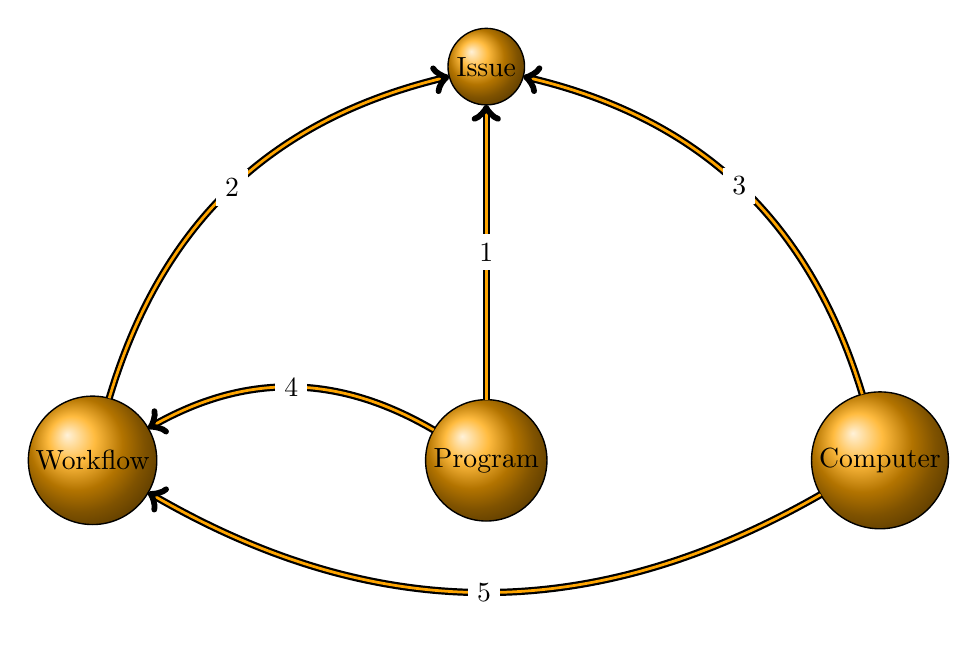
\begin{tikzpicture}
  	   	\GraphInit[vstyle = Shade]
  	   	\SetGraphUnit{5}
  	   	\Vertex{Issue}
  	   	\SOWE(Issue){Workflow}
  	   	\SO(Issue){Program}
  	   	\SOEA(Issue){Computer}
  	   	
  	   	
  	   	\Edge[label = 1, style={<-}](Issue)(Program)
  	   	\Edge[label = 2, style={<-,bend right}](Issue)(Workflow)
  	   	\Edge[label = 3, style={<-,bend left}](Issue)(Computer)
  	   	%\Edge[label = 4](Issue)(Computer)
  	   	%\Loop[dist = 4cm, dir = NO, label = 5](Computer.west)
  	   	%\Loop[dist = 4cm, dir = SO, label = 6](Program.east)
  	   	%\tikzset{EdgeStyle/.append style = {bend left = 50}}
  	   	\Edge[label = 4,style={<-,bend left}](Workflow)(Program)
  	   	\Edge[label = 5,style={->,bend left}](Computer)(Workflow)
  	   	%\Loop[dist = 4cm, dir = SOWE, label = 6](Program.west)
  	   \end{tikzpicture}}
  	\end{column}
  \end{columns}	
\end{frame}

%%%%%%%%%%%%%%%%%%%%%%%%%%%%%%%%%%%%%%%%%%%%%%%%%%%%%%%%%%%%%%%%%%%%%%%%%%%%%%%%
\begin{frame}
  \frametitle{What is the Nature of the Issue?}
  \texttt{Snakemake} helps you to identify the nature of an issue:
  \begin{enumerate}[<+->]
  	\item It will report to you in which \altverb{rule} the error occurred \textbf{and/or}
  	\item a so-called "traceback" to point the issue within its code.
  	\item The workflow will indicate log files on the screen.
  \end{enumerate}
  \pause
  \begin{docs}{Looking into Log Files}
  	Look into the log file. It \textit{should} tell you the error. \pause If not, report it to the workflow developer (next slides). 
  \end{docs}
\end{frame}

%%%%%%%%%%%%%%%%%%%%%%%%%%%%%%%%%%%%%%%%%%%%%%%%%%%%%%%%%%%%%%%%%%%%%%%%%%%%%%%%
\begin{frame}
  \frametitle{Do I need a \texttt{GitHub} account?}
  Today many software projects are either hosted on the global git server, \texttt{GitHub}.
  \begin{docs}
  	If you want to report an issue or even contribute back to the project, you will need an account. \lhref{https://docs.github.com/en/get-started/onboarding/getting-started-with-your-github-account}{This page} describes how. 
  \end{docs}
  
\end{frame}

%%%%%%%%%%%%%%%%%%%%%%%%%%%%%%%%%%%%%%%%%%%%%%%%%%%%%%%%%%%%%%%%%%%%%%%%%%%%%%%%
\begin{frame}
	\frametitle{Reporting Cluster Issues}
	\begin{question}[Where to?]
	  Report them to your cluster admins (\includegraphics[height=\texorpdfstring{\fontcharht\font`\B}]{logos/mattermost.png} chat, \Email{} mail ticket, etc.)
	\end{question}
    \pause
    \begin{question}[What?]
      Inaccessible paths (file system issue), network issues, node failures, etc. 
    \end{question}
    \pause
    \begin{question}[How?]
      Give a meaningful statement. "I can't do \altverb{ls} on \altverb{/some/path}." is more meaningful than "The filesystem stopped working!"\newline
      \bcattention Check your \Email{}! Has some maintenance been scheduled?
    \end{question}	
\end{frame}

%%%%%%%%%%%%%%%%%%%%%%%%%%%%%%%%%%%%%%%%%%%%%%%%%%%%%%%%%%%%%%%%%%%%%%%%%%%%%%%%
\begin{frame}
	\frametitle{Reporting Application Issues}
	\begin{question}[Where to?]
		The issue tracker of your application (if any). 
	\end{question}
	\pause
	\begin{question}[What?]
		Any application specific error. Try running the application with the input and parameters specified in the workflow (get them with \altverb{snakemake -p} to print the shell command or other debug flags). If the application breaks, report the failure. Else, it might be the workflow.
	\end{question}
	\pause
	\begin{question}[How?]
		Indicate the error message and what is leading to it. If you need special input to reproduce the issue, upload the input somewhere or attach minimal input to the issue report.
	\end{question}
\end{frame}

%%%%%%%%%%%%%%%%%%%%%%%%%%%%%%%%%%%%%%%%%%%%%%%%%%%%%%%%%%%%%%%%%%%%%%%%%%%%%%%%
\begin{frame}
	\frametitle{Reporting Workflow Issues}
	\begin{question}[Where to?]
		The issue tracker at your workflow. For \texttt{Snakemake} somewhere in the \lhref{https://snakemake.github.io/snakemake-workflow-catalog/}{catalog}. 
	\end{question}
	\pause
	\begin{question}[What?]
	   Check that it is you causing the error, e.\,g. undefined variables. \texttt{Snakemake} will inform you about the nature of the issue. Read the error output carefully. Report when sure it is not you.
	\end{question}
	\pause
	\begin{question}[How?]
		Indicate the error message and what is leading to it. If you need special input to reproduce the issue, upload the input somewhere or attach minimal input to the issue report.
	\end{question}
\end{frame}

%%%%%%%%%%%%%%%%%%%%%%%%%%%%%%%%%%%%%%%%%%%%%%%%%%%%%%%%%%%%%%%%%%%%%%%%%%%%%%%%
\begin{frame}
  \frametitle{Reporting \texttt{Snakemake} Issues}
  \begin{question}[Where to?]
  	 The \lhref{https://github.com/snakemake/snakemake/issues}{issue tracker of the \texttt{Snakemake} project}.
  \end{question}	
  \pause
  \begin{question}[What?]
  	Clearly unexpected behaviour. Or tracebacks pointing to \texttt{Snakemake} itself. 
  \end{question}
  \pause
  \begin{question}[How?]
  	Indicate the error message and what is leading to it (e.\,g. the command line you used). If you need special input to reproduce the issue, upload the input somewhere or attach minimal input to the issue report.
  \end{question}
\end{frame}

 
\end{document}

"
\ifdefined\ishandout
\PassOptionsToClass{handout}{beamer}
\fi

\documentclass[english,xcolor=pdftex,dvipsnames]{beamer} 

% to typeset only a few slide sets, set them here during development
%\includeonly{Why_Workflows}

\usepackage{etoolbox}
%\setbeamertemplate{mini frames}[box]
\usepackage{babel}
\usepackage[utf8]{inputenc}
\usepackage[T1]{fontenc}
\usepackage{amsfonts,amsmath,amssymb}
\usepackage{textgreek}
\usepackage{wrapfig}

\usepackage[load-configurations=binary,binary-units=true]{siunitx}
\usepackage[normalem]{ulem} % for strikethrough with \sout

\usepackage{color,colortbl}
\usepackage{upquote}

\definecolor{pblue}{RGB}{45,106,148}
\definecolor{pdarkblue}{RGB}{35,71,100}
\definecolor{plightblue}{RGB}{90,159,212}
\definecolor{pyellow}{RGB}{255,212,59}
\definecolor{pdarkyellow}{RGB}{255,188,41}
\definecolor{orange}{RGB}{255,165,0}
\definecolor{plightyellow}{RGB}{255,232,115}
\definecolor{pdarkgrey}{RGB}{100,100,100}
\definecolor{pgrey}{RGB}{153,153,153}
\definecolor{plightgrey}{RGB}{233,233,233}
\definecolor{plightgrey2}{RGB}{247,247,247}
\definecolor{pnavy}{RGB}{0,0,170}
\definecolor{BrickRed}{RGB}{150,22,11}
\definecolor{BlueViolet}{RGB}{138, 43, 226}
\definecolor{PineGreen}{RGB}{0, 51, 0}
\definecolor{light-gray}{gray}{0.95}

\definecolor{UniRot}{RGB}{193,0,42}
\definecolor{UniDunkelGrau}{RGB}{99,99,99}
\definecolor{UniHellGrau}{RGB}{172,172,172}

\definecolor{UrlColor}{rgb}{0,0.08,0.45}
\definecolor{links}{rgb}{0,0,0}

\usetheme{CambridgeUS} % Pittsburgh, CambridgeUS
\usecolortheme{beaver} %wolverine | crane | beaver | seahorse
\useinnertheme{rounded} 
\useoutertheme{default}
\usefonttheme{default}
%\setbeamercovered{transparent}
\setbeamertemplate{footline}[frame number]

% remove the navigation symbols
\setbeamertemplate{navigation symbols}{}

% side margins
\setbeamersize{text margin left=0.5cm, text margin right=0.5cm}

\setbeamercolor{structure}{fg=UniRot}% to modify  immediately all palettes
\setbeamercolor{title}{fg=UniRot}
\setbeamercolor{title in head/foot}{fg=UniRot}

\setbeamercolor{block title}{bg=UniRot!20,fg=darkred}
\setbeamercolor{block body}{fg=black, bg=plightgrey2}

% \setbeamercolor{block title}{fg=white,bg=orange}
\setbeamercolor{block title alerted}{fg=white,bg=UniRot}
\setbeamercolor{block title example}{fg=white,bg=PineGreen!80}


% enables two line cols in tabular envs
\newcommand{\specialcell}[2][c]{%
  \begin{tabular}[#1]{@{}c@{}}#2\end{tabular}}
\usepackage{subfig}
\usepackage{tikz}
\usetikzlibrary{arrows,shapes,backgrounds,positioning,shadows,decorations,trees,decorations.pathreplacing}
\usepackage{tkz-graph}

\usepackage{smartdiagram}


\addtobeamertemplate{footline}{}{%
\begin{tikzpicture}[remember picture,overlay]
\node[anchor=south west,yshift=2pt] at (current page.south west) {\includegraphics[height=0.8cm]{../images/logos/zdv_logo.png}};
\end{tikzpicture}}

\usepackage[tikz]{bclogo}
\newenvironment{task}[1][Task]{\bclogo[arrondi=0.1,logo=\bcoutil]{#1}}{\endbclogo}
\newenvironment{docs}[1][Documentation]{\bclogo[arrondi=0.1,logo=\bcplume]{#1}}{\endbclogo}
\newenvironment{hint}[1][Hint]{\bclogo[arrondi=0.1,logo=\bcinfo]{#1}}{\endbclogo}
\newenvironment{warning}[1][Warning]{\bclogo[arrondi=0.1,logo=\bcattention]{#1}}{\endbclogo}
% ``d/Definition'' is already defined ;-)
\newenvironment{explanation}[1][Definition]{\bclogo[arrondi=0.1,logo=\bcplume]{#1}}{\endbclogo}
\newenvironment{question}[1][Question]{\bclogo[arrondi=0.1,logo=\bcquestion]{#1}}{\endbclogo}


%%%%%%%%%%%%%%%%%
%% PLEASE NOTE %%
%%%%%%%%%%%%%%%%%
% frames containing ``Hand Out'' or ``Interlude'' should be started:

% \setcounter{preframe_handson}{\value{handson}}
% \begin{frame}[fragile]
%   \setcounter{handson}{\value{preframe_handson}}
%   \frametitle{\HandsOn{Using \texttt{find}}}

% or

% \setcounter{preframe_interlude}{\value{interlude}}
% \begin{frame}[fragile]
%   \setcounter{interlude}{\value{preframe_interlude}}
%   \frametitle{Interlude -- Parameter Extension}

% respectively.

\newcounter{handson}
\setcounter{handson}{1}
\newcounter{preframe_handson}
\setcounter{preframe_handson}{1}
\newcommand{\HandsOn}[1]{Hands On \Roman{handson} -- #1 \addtocounter{handson}{1}}
%\newcommand{\HandsOn}[1]{Hands On -- #1}

%TODO: Merge ``HandsOn'' && ``Excercise''
\newcounter{exercise}
\setcounter{exercise}{1}
% \newcommand{\Exercise}{\theexercise . Excercise \addtocounter{exercise}{1}}

% Bugfix of the Exercise command: avoid the annoying counter
\newcommand{\Exercise}{\theexercise . Excercise \addtocounter{exercise}{1}}

\newcounter{interlude}
\setcounter{interlude}{1}
\newcounter{preframe_interlude}
\setcounter{preframe_interlude}{1}

%\newcommand{\Interlude}[1]{Interlude \Roman{interlude} -- #1 \addtocounter{interlude}{1}}

% Bugfix of the Interlude command: avoid the annoying counter!
\newcommand{\Interlude}[1]{Interlude -- #1}

\usepackage{marvosym}
\usepackage{multicol}

\usepackage{hhline}

\usepackage{times}

% will decrease the font size for one frame
\newcommand\Fontvi{\fontsize{6}{7.2}\selectfont}
% 
\usepackage{dirtree,float} % for directory tree listings
\usepackage[nodisplayskipstretch]{setspace}


\usepackage{verbatim}
\usepackage{listings}

\newcommand{\altverb}[2][{}]{\colorbox{plightgrey}{\lstinline[language={#1}]{#2}}}


\lstloadlanguages{Python,bash,C++}
\lstset{showspaces=false,
basicstyle=\small,
showstringspaces=false}

\lstdefinestyle{tree}{
    literate=
    {├}{{smash{raisebox{-1ex}{rule{1pt}{baselineskip}}}raisebox{0.5ex}{rule{1ex}{1pt}}}}1 
    {─}{{raisebox{0.5ex}{rule{1.5ex}{1pt}}}}1 
    {└}{{smash{raisebox{0.5ex}{rule{1pt}{dimexprbaselineskip-1.5ex}}}raisebox{0.5ex}{rule{1ex}{1pt}}}}1 
  }

%default python listings:
\lstdefinestyle{Python}
{
  language=Python,
  basicstyle=\small,
  showstringspaces=false,
  stepnumber=5,
  numberstyle=\tiny,
  numbersep=5pt,
  showspaces=false,
  frame=single,
  framerule=0.4pt,
  rulecolor=\color{pgrey},
  backgroundcolor=\color{white},
  stringstyle=\color{BrickRed},
  keywordstyle=\color{BlueViolet}\bfseries,
  commentstyle=\color{PineGreen}\bfseries,
  identifierstyle={},
  emph={[10]self}, emphstyle={[10]\color{pblue}},
  emph={[11]yield}, emphstyle={[11]\color{pblue}},
  moredelim=**[is][\bfseries\color{red}]{@}{@},
  literate={\\@}{{\makeatletter @ \makeatother}}1
}

\lstdefinestyle{R}
{
  language=R,
  basicstyle=\small,
  showstringspaces=false,
  stepnumber=5,
  numberstyle=\tiny,
  numbersep=5pt,
  showspaces=false,
  frame=single,
  framerule=0.4pt,
  rulecolor=\color{pgrey},
  backgroundcolor=\color{white},
  stringstyle=\color{BrickRed},
  keywordstyle=\color{BlueViolet}\bfseries,
  commentstyle=\color{PineGreen}\bfseries,
  identifierstyle={},
  emph={[10]self}, emphstyle={[10]\color{pblue}},
  emph={[11]yield}, emphstyle={[11]\color{pblue}},
}

%default python listings:
\lstdefinestyle{C++}
{
  language=C++,
  basicstyle=\small,
  showstringspaces=false,
  stepnumber=5,
  numberstyle=\tiny,
  numbersep=5pt,
  showspaces=false,
  frame=single,
  framerule=0.4pt,
  rulecolor=\color{pgrey},
  backgroundcolor=\color{white},
  stringstyle=\color{BrickRed},
  keywordstyle=\color{BlueViolet}\bfseries,
  commentstyle=\color{PineGreen}\bfseries,
  identifierstyle={},
  emph={[10]self}, emphstyle={[10]\color{pblue}},
  emph={[11]yield}, emphstyle={[11]\color{pblue}},
}

\newcommand{\CC}{C\nolinebreak\hspace{-.05em}\raisebox{1ex}{\tiny\bf +}\nolinebreak\hspace{-.10em}\raisebox{1ex}{\tiny\bf +}}

%default shell listings:
\lstdefinestyle{Shell}
{
  language=Bash,
  basicstyle=\ttfamily\small,
  showstringspaces=false,
  frame=single,
  framerule=0.4pt,
  rulecolor=\color{pgrey},
  backgroundcolor=\color{plightgrey2},
  stringstyle=\color{BrickRed},
  keywordstyle=\color{BlueViolet},
  commentstyle=\color{PineGreen}\bfseries,
  identifierstyle=\color{black},
  emph={[10]\$,>>>}, emphstyle={[10]\color{pblue}},
  moredelim=**[is][\bfseries\color{red}]{@}{@},
  literate={\\@}{{\makeatletter @ \makeatother}}1
}

%default plain listings (e.g. for config files):https://www.google.com/search?client=firefox-b-e&q=conrad
\lstdefinestyle{Plain}
{ 
  stepnumber=5,
  numberstyle=\tiny,
  numbersep=5pt,
  language=Bash,
  basicstyle=\ttfamily\small,
  showstringspaces=false,
  frame=single,
  framerule=0.4pt,
  rulecolor=\color{pgrey},
  backgroundcolor=\color{plightgrey2},
  stringstyle=\color{black},
  keywordstyle=\color{black},
  commentstyle=\color{blue}\bfseries,
  identifierstyle=\color{black},
  breaklines=true,
  emph={[10]\$,>>>}, emphstyle={[10]\color{pblue}}
}

\lstdefinelanguage{XML}
{
  frame=single,
  framerule=0.4pt,
  rulecolor=\color{pgrey},
  backgroundcolor=\color{plightgrey2},
  stringstyle=\color{black},
  keywordstyle=\color{black},
  commentstyle=\color{blue}\bfseries,
  identifierstyle=\color{black},
  emph={[10]\$,>>>}, emphstyle={[10]\color{pblue}}
  morestring=[b]",
  morestring=[s]{>}{<},
  morecomment=[s]{<?}{?>},
  morekeywords={xmlns,version,type}% list your attributes here
}

\newcommand{\bibtex}{\textsc{Bib}\TeX}

%%% https://tex.stackexchange.com/questions/99316/symbol-for-external-links
\newcommand{\LinkSymbol}{%
  \tikz[x=1.2ex, y=1.2ex, baseline=-0.05ex]{% 
    \begin{scope}[x=1ex, y=1ex]
      \clip (-0.1,-0.1) 
      --++ (-0, 1.2) 
      --++ (0.6, 0) 
      --++ (0, -0.6) 
      --++ (0.6, 0) 
      --++ (0, -1);
      \path[draw, 
      line width = 0.5, 
      rounded corners=0.5] 
      (0,0) rectangle (1,1);
    \end{scope}
    \path[draw, line width = 0.5] (0.5, 0.5) 
    -- (1, 1);
    \path[draw, line width = 0.5] (0.6, 1) 
    -- (1, 1) -- (1, 0.6);
  }
}
\newcommand{\lhref}[2]{\href{#1}{#2\,\LinkSymbol}}

%%%% shortcuts for uniform appearance of common strings %%%%
\newcommand{\slurm}{\textsc{slurm}~}
\makeatletter
\newcommand{\rmnum}[1]{\romannumeral #1}
\newcommand{\Rmnum}[1]{\expandafter\@slowromancap\romannumeral #1@}
\makeatother

% this package provides the option to read parameters from a configuration file
\usepackage{readarray}

\readdef{config/config.dat}{\data}
\readarray\data\MyDat[-,3]
\newcommand\configparam[1]{\csname DATA#1\endcsname}
%\MyDatROWS{} rows of data read.

\newcounter{datacount}
\setcounter{datacount}{0}%
\whiledo{\value{datacount} < \MyDatROWS}{%
	\stepcounter{datacount}%
	\expandafter\xdef\csname DATA\MyDat[\arabic{datacount},1]\endcsname{%
		\MyDat[\arabic{datacount},3]}%
}



%\newcommand{\pathtoexercise}[1]{\path{/lustre/project/m2_jgu-ngstraing/workflows/#1}}
%\newcommand{\pathtoexercise}[1]{\path{ \DTLfetch{data}{thekey}{#1}{thevalue}   }}
%\newcommand{\pathtoclozure}[1]{\path{/lustre/project/hpckurs/bash-course/cloze/#1}}
%\newcommand{\pathtosolution}[1]{\path{/lustre/project/hpckurs/bash-course/solutions/#1}}

\setcounter{tocdepth}{1}

% this allows turning of footlines for particular slides
\setbeamertemplate{footline}[frame number]
% to use it, perform:

% \begin{frame}
% normal frame
% \end{frame}
% 
% \begingroup
% \setbeamertemplate{footline}{}
% \begin{frame}
% without footline
% \end{frame}
% \endgroup

%--------------------%
% Meta-Info 
%--------------------%



\title[Introduction to Workflow Programming]{An Introduction to HPC-conformant Scientific Workflows} 
%TODO: What should the subtitle be like? Should there be an Edition? How to keep track?
\subtitle{Workflow Course - Edition 3} 
\author[Snakemake Teaching Alliance]{The "Snakemake Teaching Alliance"}
% TODO: How do we insert a date, which is up to date? Should we insert one, here?
\date{September 2023}

\hypersetup{colorlinks,linkcolor=,urlcolor=links}

\graphicspath{{../images/}{../logos}}


% Passe captions an
\setbeamertemplate{caption}{\insertcaption}
% \setbeamerfont{caption}{size=\scriptsize}
\setlength\abovecaptionskip{-2.5pt}
\setlength\belowcaptionskip{0pt}



% For every picture that defines or uses external nodes, you'll have to
% apply the 'remember picture' style. To avoid some typing, we'll apply
% the style to all pictures.
\tikzstyle{every picture}+=[remember picture]
\tikzstyle{na} = [baseline=-.5ex]


\title[<++course.shorttitle++>]{<+++ if course.title is defined +++><++course.tittle++><+++else+++>An Introduction to HPC-conformant Scientific Workflows with \Snakemake<+++endif+++>} 

\subtitle{<+++ if course.subtitle is defined +++><++course.subtitle++><+++else+++>Programming and Deployment<+++endif+++> - <++course.edition++>} 

%%%%%%%%%%%%%%%%%%%%%%%%%%%%%%%%%%%%%%%%%%%%%%%%%%%%%%%%%%%%%%%%%%%%%%%%%%%%%%%%
%%%%%%%%%%%%%%%%%%%%%%%%%%%%%%%%%%%%%%%%%%%%%%%%%%%%%%%%%%%%%%%%%%%%%%%%%%%%%%%%
\begin{document}
%%%%%%%%%%%%%%%%%%%%%%%%%%%%%%%%%%%%%%%%%%%%%%%%%%%%%%%%%%%%%%%%%%%%%%%%%%%%%%%%
%%%%%%%%%%%%%%%%%%%%%%%%%%%%%%%%%%%%%%%%%%%%%%%%%%%%%%%%%%%%%%%%%%%%%%%%%%%%%%%%

% attempts a better type setting for hboxes (might result in less overful warnings)
\sloppy

%%%%%%%%%%%%%%%%%%%%%%%%%%%%%%%%%%%%%%%%%%%%%%%%%%%%%%%%%%%%%%%%%%%%%%%%%%%%%%%% 
\begin{frame}[plain] % plain erzeugt Titelseite ohne Kopf- und Fußzeile
  \titlepage
\end{frame}

%%%%%%%%%%%%%%%%%%%%%%%%%%%%%%%%%%%%%%%%%%%%%%%%%%%%%%%%%%%%%%%%%%%%%%%%%%%%%%%%
%%%%%%%%%%%%%%%%%%%%%%%%%%%%%%%%%%%%%%%%%%%%%%%%%%%%%%%%%%%%%%%%%%%%%%%%%%%%%%%%
\section{Contributors}

%%%%%%%%%%%%%%%%%%%%%%%%%%%%%%%%%%%%%%%%%%%%%%%%%%%%%%%%%%%%%%%%%%%%%%%%%%%%%%%%
\begin{frame}
  \frametitle{Honour where Honour is due}
  \begin{columns}
  	\begin{column}{.5\textwidth}
  	   \begin{itemize}
  	   	\item Johannes Köster \includegraphics[height=\baselineskip]{logos/signet_ude_rgb}
  	   	\item Lukas Hellmann \includegraphics[height=\baselineskip]{logos/logo_schriftzug.jpg}
  	   	\item Christian Meesters \includegraphics[height=\baselineskip]{logos/logo_schriftzug.jpg}
  	   	\item Malte Petersen \includegraphics[height=\baselineskip]{logos/UNI_Bonn_Logo_Standard+HPCA.pdf}
  	   	\item Fabian Brand \includegraphics[height=\baselineskip]{logos/UNI_Bonn_Logo_Standard+HPCA.pdf}
  	   	\item Florian Boecker \includegraphics[height=\baselineskip]{logos/UNI_Bonn_Logo_Standard_RZ.pdf}
  	   \end{itemize}	
  	\end{column}
    \begin{column}{.5\textwidth}
    	\begin{itemize}
    		\item See how to contribute \lhref{https://github.com/cmeesters/snakemake-hpc-teaching-material}{on our repository.}
    	\end{itemize}	
    \end{column}
  \end{columns}
		
\end{frame}



%%%%%%%%%%%%%%%%%%%%%%%%%%%%%%%%%%%%%%%%%%%%%%%%%%%%%%%%%%%%%%%%%%%%%%%%%%%%%%%%
%%%%%%%%%%%%%%%%%%%%%%%%%%%%%%%%%%%%%%%%%%%%%%%%%%%%%%%%%%%%%%%%%%%%%%%%%%%%%%%%
{   
	\usebackgroundtemplate{
		\vbox to \paperheight{\vfil\hbox to \paperwidth{\hfil\includegraphics[height=\paperheight]{humor/DALLE_frustration_to_heureka.jpg}\hfil}\vfil}
		
	}
	\frame{
		\frametitle{Before we begin \ldots}
		\vspace{8.5em}
		\begin{mdframed}[tikzsetting={draw=white,fill=white,fill opacity=0.8,
				line width=0pt},backgroundcolor=none,leftmargin=0,
			rightmargin=50,innertopmargin=4pt,roundcorner=10pt]
			Yes, you will make mistakes. This is \ldots
			\begin{itemize}
				\item normal (it happens to \emph{all} of us)
				\item no reason to despair - you / we can learn from mistakes!
				\item just a reason to ask
			\end{itemize}
		\end{mdframed}
	    \vfill\hfil \hfill{\tiny image: own creation with DALL-E}
	}
}

%%%%%%%%%%%%%%%%%%%%%%%%%%%%%%%%%%%%%%%%%%%%%%%%%%%%%%%%%%%%%%%%%%%%%%%%%%%%%%%%
\section{Why Workflows}

%%%%%%%%%%%%%%%%%%%%%%%%%%%%%%%%%%%%%%%%%%%%%%%%%%%%%%%%%%%%%%%%%%%%%%%%%%%%%%%%
\begin{frame}
    \frametitle{Outline}
    \begin{columns}[t]
        \begin{column}{.5\textwidth}
            \tableofcontents[sections={1-9},currentsection]
        \end{column}
        \begin{column}{.5\textwidth}
            \tableofcontents[sections={10-18},currentsection]
        \end{column}
    \end{columns}
\end{frame}

%%%%%%%%%%%%%%%%%%%%%%%%%%%%%%%%%%%%%%%%%%%%%%%%%%%%%%%%%%%%%%%%%%%%%%%%%%%%%%%%
\begin{frame}
  \frametitle{What is this about?}
   \begin{question}[Questions]
   	 \begin{itemize}
        \item I can code everything! Can I?
        \item What is the benefit of a workflow system?
        \item What distinguishes a workflow system from a ``pipeline''?
     \end{itemize}
   \end{question}
   \docs[Objectives]{\begin{enumerate}
                      \item Introducing workflow engines (particularly \texttt{Snakemake})!
                     \end{enumerate}}
\end{frame}  

%%%%%%%%%%%%%%%%%%%%%%%%%%%%%%%%%%%%%%%%%%%%%%%%%%%%%%%%%%%%%%%%%%%%%%%%%%%%%%%%
\begin{frame}
  \frametitle{Data Analysis}
  \begin{onlyenv}<1| handout:0>
    \begin{tikzpicture}
      \path[use as bounding box] (0.7,0) rectangle (12,8);
      \node[inner sep=0pt] (analysis_1) at (5,6)
         {\includegraphics[width=0.7\textwidth]{Snakemake/analysis_1.png}};   
      \node at (7, 3.5) %[below=-0.4cm of analysis_1, xshift=2.7cm] at (current page.center)
         {\includegraphics[width=0.45\textwidth]{Snakemake/phd_left.png}};
      \node at (6, 1) {\begin{minipage}{0.75\textwidth}\footnotesize
                        Idea from the official \lhref{https://slides.com/johanneskoester/snakemake-tutorial}{\texttt{Snakemake}} course (with permission), image from \lhref{https://phdcomics.com/comics.php}{PhD comics}.
                       \end{minipage}
      };
    \end{tikzpicture}    
  \end{onlyenv}
  
  \begin{onlyenv}<2| handout:1>
    \begin{tikzpicture}
      \path[use as bounding box] (0.7,0) rectangle (12,8);
      \node[inner sep=0pt] (analysis_full) at (5,6)
         {\includegraphics[width=0.7\textwidth]{Snakemake/analysis_full.png}};   
      \node at (7,3.5) % [below=-0.4cm of analysis_full, xshift=2.7cm]
         {\includegraphics[width=0.45\textwidth]{Snakemake/phd_full.png}};
      \node at (6, 1) {\begin{minipage}{0.75\textwidth}\footnotesize
                        Idea from the official \lhref{https://slides.com/johanneskoester/snakemake-tutorial}{\texttt{Snakemake}} course (with permission), image from \lhref{https://phdcomics.com/comics.php}{PhD comics}.
                       \end{minipage}
      };
    \end{tikzpicture}
  \end{onlyenv}
\end{frame}

%%%%%%%%%%%%%%%%%%%%%%%%%%%%%%%%%%%%%%%%%%%%%%%%%%%%%%%%%%%%%%%%%%%%%%%%%%%%%%%%
\begin{frame}
  \frametitle{Goals of Reproducibility}
  \Huge
  \begin{enumerate}
   \item Dispel Doubts
   \item Facilitate Further Experimentation
  \end{enumerate}
  \vfill
  \footnotesize{Idea from \lhref{https://elephly.net/downies/2023-dfn-slides.pdf}{DFN slides}.}
\end{frame}

%%%%%%%%%%%%%%%%%%%%%%%%%%%%%%%%%%%%%%%%%%%%%%%%%%%%%%%%%%%%%%%%%%%%%%%%%%%%%%%%
\begin{frame}
  \frametitle{Reproducible Data Analysis}
  \begin{onlyenv}<1| handout:0>
    \begin{tikzpicture}
      \path[use as bounding box] (0.7,0) rectangle (12,8);
      \node at (5.5, 5.5) {\includegraphics[width=0.7\textwidth]{Snakemake/automation.png}};
      \node at (8, 2.5) {\begin{minipage}{0.65\textwidth}
                             \textbf{From raw data to final figures:}
                             \begin{itemize}
                                \item \textbf{document} parameters, tools, versions
                                \item \textbf{execute} without manual intervention
                              \end{itemize}
                           \end{minipage}
                           };
    \end{tikzpicture}
  \end{onlyenv}
  \begin{onlyenv}<2| handout:0>
    \begin{tikzpicture}
      \path[use as bounding box] (0.7,0) rectangle (12,8);
      \node at (5.5, 5.5) {\includegraphics[width=0.7\textwidth]{Snakemake/scalability.png}};
      \node at (8, 2.5) {\begin{minipage}{0.65\textwidth}
                             \textbf{Handle parallelization:}
                             \begin{itemize}
                                \item execute for tens of thousands of datasets
                                \item efficiently use any computing platform
                              \end{itemize}
                           \end{minipage}
                           };
    \end{tikzpicture}
  \end{onlyenv}
  \begin{onlyenv}<3| handout:1>
    \begin{tikzpicture}
      \path[use as bounding box] (0.7,0) rectangle (12,8);
      \node at (5.5, 5.5) {\includegraphics[width=0.7\textwidth]{Snakemake/portability.png}};
      \node at (8, 2.5) {\begin{minipage}{0.65\textwidth}
                             \textbf{Handle deployment:}\newline
                             be able to easily execute analyses on a different system/platform/infrastructure
                           \end{minipage}
                           };
    \end{tikzpicture}
  \end{onlyenv}
\end{frame}

%%%%%%%%%%%%%%%%%%%%%%%%%%%%%%%%%%%%%%%%%%%%%%%%%%%%%%%%%%%%%%%%%%%%%%%%%%%%%%%%
\begin{frame}
  \frametitle{Beyond Reproducibility}
  \begin{onlyenv}<1| handout:0>
    \begin{figure}
      \centering
      \includegraphics[width=0.85\textwidth]{Snakemake/reproducibility_only.png}
    \end{figure}
  \end{onlyenv}
  \begin{onlyenv}<2| handout:0>
    \begin{figure}
      \centering
      \includegraphics[width=0.85\textwidth]{Snakemake/reproducibility_empty.png}
    \end{figure}
  \end{onlyenv}
  \begin{onlyenv}<3| handout:0>
    \begin{figure}
      \centering
      \includegraphics[width=0.85\textwidth]{Snakemake/reproducibility_left.png}
    \end{figure}
  \end{onlyenv}
    \begin{onlyenv}<4| handout:1>
      \begin{figure}
        \centering
        \includegraphics[width=0.85\textwidth]{Snakemake/reproducibility_full.png}
      \end{figure}
  \end{onlyenv}
\end{frame}

%%%%%%%%%%%%%%%%%%%%%%%%%%%%%%%%%%%%%%%%%%%%%%%%%%%%%%%%%%%%%%%%%%%%%%%%%%%%%%%%
\begin{frame}
  \frametitle{\textbf{Snakemake}}
  \begin{figure}
    \centering
    \caption{\textbf{>370k} downloads since 2015\newline
             \textbf{>1300} citations\newline
             \textbf{>7} citations per week since 2021}
    \includegraphics[width=0.6\textwidth]{Snakemake/paper_wall.png}
  \end{figure}
\end{frame}

%%%%%%%%%%%%%%%%%%%%%%%%%%%%%%%%%%%%%%%%%%%%%%%%%%%%%%%%%%%%%%%%%%%%%%%%%%%%%%%%
\begin{frame}
  \frametitle{The \includegraphics[width=2em]{logos/Snakemake.png} Catalogue}
  \begin{columns}
    \begin{column}{0.5\textwidth}
      \begin{itemize}[<+->]
   \item extremely feature rich
   \item over 1800 workflows in \lhref{https://snakemake.github.io/snakemake-workflow-catalog/}{its catalogue}
   \item almost a hundred standardized (meaning: will documented and with automatic deployment)
   \item cluster batch systems are supported (and support for various cloud systems, too)
   \item there is an option to include Nextflow wrappers, too.
      \end{itemize}
    \end{column}
    \begin{column}{0.5\textwidth}
      \begin{figure}
        \includegraphics[width=\textwidth]{Snakemake/Snakemake_Workflow_Catalog.png}
        \caption{Screenshot of the Workflow Catalogue}
      \end{figure}
    \end{column}
  \end{columns}
\end{frame}


%%%%%%%%%%%%%%%%%%%%%%%%%%%%%%%%%%%%%%%%%%%%%%%%%%%%%%%%%%%%%%%%%%%%%%%%%%%%%%%%
\subsection{Goals, Background \& Outline}

%%%%%%%%%%%%%%%%%%%%%%%%%%%%%%%%%%%%%%%%%%%%%%%%%%%%%%%%%%%%%%%%%%%%%%%%%%%%%%%%
\begin{frame}
  \frametitle{Questions}
  \begin{question}[The questions you most probably have when starting your Analysis:]
  	\begin{itemize}
      \item How to start quickly (with the lowest amount of overhead)?
      \item What are the necessary tools?
    \end{itemize}
  \end{question}
                                                                               
  \begin{question}[Our question to you:]
  	 How do you get this information? And: Is reproducibility and sustainability your concern?
  \begin{question}
  \pause
  \begin{block}{Most frequent Sources}
   \begin{itemize}
    \item Your labmate(s)
    \item The Internet
    \item Yes, of course ... eventually, when I brag about my paper/thesis.
   \end{itemize}
  \end{block}
\end{frame}

%%%%%%%%%%%%%%%%%%%%%%%%%%%%%%%%%%%%%%%%%%%%%%%%%%%%%%%%%%%%%%%%%%%%%%%%%%%%%%%%
\begin{frame}
  \frametitle{The Workflow Approach}
  Workflow Engines answer these questions directly by providing
  \begin{itemize}
   \item entire Workflows can be selected and can be put to action.
   \item executing routines reliably.
  \end{itemize}
\end{frame}

%%%%%%%%%%%%%%%%%%%%%%%%%%%%%%%%%%%%%%%%%%%%%%%%%%%%%%%%%%%%%%%%%%%%%%%%%%%%%%%%
\begin{frame}
  \frametitle{Going HPC}
  \begin{question}
  	Why would you want to work on a cluster?
  \end{question}
  \pause
  Answers may include:
  \begin{itemize}[<+->]
   \item compute power and ressources for big data
   \item launching scalable (and otherwise portable) workflows with workflow engines
  \end{itemize}
\end{frame}


%%%%%%%%%%%%%%%%%%%%%%%%%%%%%%%%%%%%%%%%%%%%%%%%%%%%%%%%%%%%%%%%%%%%%%%%%%%%%%%%
%%%%%%%%%%%%%%%%%%%%%%%%%%%%%%%%%%%%%%%%%%%%%%%%%%%%%%%%%%%%%%%%%%%%%%%%%%%%%%%%
\section{About Snakemake}
{   
	\usebackgroundtemplate{
		\vbox to \paperheight{\vfil\hbox to \paperwidth{\hfil\includegraphics[height=\paperheight]{logos/Wild_Python.jpg}\hfil}\vfil}
	}
	\frame{
		\frametitle{Snakemake}
		\begin{mdframed}[tikzsetting={draw=white,fill=white,fill opacity=0.8,
				line width=0pt},backgroundcolor=none,leftmargin=0,
			rightmargin=150,innertopmargin=4pt,roundcorner=10pt]
			\tableofcontents[currentsection,sections={1-4},hideothersubsections]
		\end{mdframed}
	}
}

%%%%%%%%%%%%%%%%%%%%%%%%%%%%%%%%%%%%%%%%%%%%%%%%%%%%%%%%%%%%%%%%%%%%%%%%%%%%%%%%
\begin{frame}
	\frametitle{What is this about?}
	\begin{question}[Questions]
		\begin{itemize}
			\item Why \Snakemake?
			\item Why not "Something Else"?
			\item Why Clusters?
		\end{itemize}
	\end{question}
	\begin{docs}[Objectives]
		\begin{enumerate}
			\item Introduction to \Snakemake Usage (in-depth will follow)
			\item Get an Mini-Overview about Workflow Systems
		\end{enumerate}
	\end{docs}
\end{frame}

\subsection{\Snakemake and the Workflow Catalogue}

%%%%%%%%%%%%%%%%%%%%%%%%%%%%%%%%%%%%%%%%%%%%%%%%%%%%%%%%%%%%%%%%%%%%%%%%%%%%%%%%
\begin{frame}
	\frametitle{\Snakemake}
	\begin{figure}
		\centering
		\caption*{\textbf{>1e6} downloads since 2015\newline
			\textbf{>1300} citations\newline
			\textbf{>7} citations per week since 2021}
		\includegraphics[width=0.6\textwidth]{Snakemake/paper_wall.png}
	\end{figure}
\end{frame}

%%%%%%%%%%%%%%%%%%%%%%%%%%%%%%%%%%%%%%%%%%%%%%%%%%%%%%%%%%%%%%%%%%%%%%%%%%%%%%%%
\begin{frame}
	\frametitle{\Snakemake is a NumFocus-Partner}
	\begin{columns}
		\begin{column}{0.5\textwidth}
			\includegraphics[width=.95\textwidth]{logos/NumFocus_LRG_WHITE-BG.png}
		\end{column}
	    \begin{column}{0.5\textwidth}
	    	\pause
	    	Partnered and in parts funded along projects like:
	    	\includegraphics[width=.95\textwidth]{logos/numfocus_projects.png}
	    \end{column}
	\end{columns}
\end{frame}

%%%%%%%%%%%%%%%%%%%%%%%%%%%%%%%%%%%%%%%%%%%%%%%%%%%%%%%%%%%%%%%%%%%%%%%%%%%%%%%%
\begin{frame}
	\frametitle{The \Snakemake{} Catalogue}
	\begin{columns}
		\begin{column}{0.5\textwidth}
			\begin{itemize}[<+->]
				\item Extremely feature rich: \lhref{https://snakemake.github.io/snakemake-workflow-catalog/}{over 1800 workflows}
				\item Almost a hundred standardized workflows ready to use (meaning: well documented and with automatic deployment)
				\item Cluster batch systems are supported (and support for various cloud systems, too)
				\item There is an option to include Nextflow wrappers, too.
			\end{itemize}
		\end{column}
		\begin{column}{0.5\textwidth}
			\begin{figure}
				\includegraphics[width=\textwidth]{Snakemake/Snakemake_Workflow_Catalog.png}
				\caption*{Screenshot of the Workflow Catalogue}
			\end{figure}
		\end{column}
	\end{columns}
\end{frame}

%%%%%%%%%%%%%%%%%%%%%%%%%%%%%%%%%%%%%%%%%%%%%%%%%%%%%%%%%%%%%%%%%%%%%%%%%%%%%%%%
\subsection{Background}

%%%%%%%%%%%%%%%%%%%%%%%%%%%%%%%%%%%%%%%%%%%%%%%%%%%%%%%%%%%%%%%%%%%%%%%%%%%%%%%%
\begin{frame}[fragile]
	\frametitle{How does \Snakemake on a Cluster work?}
	\begin{columns}[T]
		\begin{column}{.5\textwidth}
			\begin{itemize}[<+->]
				\item Snakemake is triggered on the command line:
				\begin{lstlisting}[language=Bash, style=Shell]
$ snakemake [<arguments>]
				\end{lstlisting} 
			    \item you will fill in the parameters of your workflow (in a file)
			    \item Snakemake will run on the login-node and spawn your jobs on the cluster 
			\end{itemize}
			
		\end{column}
		\begin{column}{.5\textwidth}
			\only<3>{\includegraphics[width=0.95\textwidth]{misc/cluster_scheme.png}}
		\end{column}
	\end{columns}
\end{frame}

%%%%%%%%%%%%%%%%%%%%%%%%%%%%%%%%%%%%%%%%%%%%%%%%%%%%%%%%%%%%%%%%%%%%%%%%%%%%%%%%
\begin{frame}<handout:0>
  \frametitle{"Spawn Jobs on a Cluster?!" - What does it mean?}
  \centering
  \begin{tabular}{m{0.1\textwidth} m{0.25\textwidth} m{0.2\textwidth} m{0.45\textwidth}}
PC: & \includegraphics[width=0.1\textwidth]{misc/pc_color.png}  	    &  \includegraphics[width=0.15\textwidth]{misc/sequential_code.png} &  \begin{minipage}{0.45\textwidth}
	$\Rightarrow$ sequential code \newline
	(perhaps parallel)
\end{minipage} \\ \pause
 	
Server: & \includegraphics[width=0.1\textwidth]{misc/homeserver.png}  	&  \includegraphics[width=0.15\textwidth]{misc/concurrent.pdf} & \begin{minipage}{0.45\textwidth}
	$\Rightarrow$ sequential code \newline(perhaps parallel), \newline some concurrency
	\end{minipage}\\ \pause
  	
Cluster: & \includegraphics[width=0.1\textwidth]{misc/data_center.png}  	&  \includegraphics[width=0.15\textwidth]{misc/high_concurrent.pdf} & \begin{minipage}{0.45\textwidth}
	$\Rightarrow$ programs launched \newline with high parallelism, \newline high concurreny
	\end{minipage}\\
  \end{tabular}
\end{frame}

%%%%%%%%%%%%%%%%%%%%%%%%%%%%%%%%%%%%%%%%%%%%%%%%%%%%%%%%%%%%%%%%%%%%%%%%%%%%%%%%
\begin{frame}
   \frametitle{Benefit of Cluster Usage}
   \begin{columns}
   	 \begin{column}{0.6\textwidth}
   	 	\centering
   	 	\includegraphics[width=0.8\textwidth]{workflows/molecular_screening_dag.jpeg}
   	 \end{column}
     \begin{column}{0.6\textwidth}
     	{\footnotesize
     		\Snakemake offers
     		\begin{itemize}[<+->]
     		  \item to carry out Nextflow wrappers
     		  \item to react on your input \newline $\Rightarrow$  more samples, more jobs
     		  \item to be a remedy to I/O contention
     		  \item to be ready for real time \newline computation with cluster support
     		  \item to support you from your input \newline to publication
     		  \item \ldots
     		\end{itemize}
     	}
     \end{column}
   \end{columns}
\end{frame}
	

%%%%%%%%%%%%%%%%%%%%%%%%%%%%%%%%%%%%%%%%%%%%%%%%%%%%%%%%%%%%%%%%%%%%%%%%%%%%%%%%
\include{<++course.editorfile++>}

%%%%%%%%%%%%%%%%%%%%%%%%%%%%%%%%%%%%%%%%%%%%%%%%%%%%%%%%%%%%%%%%%%%%%%%%%%%%%%%%
\section{Software Environment}

%%%%%%%%%%%%%%%%%%%%%%%%%%%%%%%%%%%%%%%%%%%%%%%%%%%%%%%%%%%%%%%%%%%%%%%%%%%%%%%%
\begin{frame}
	\frametitle{Outline}
	\begin{columns}[t]
		\begin{column}{.5\textwidth}
			\tableofcontents[sections={1-9},currentsection]
		\end{column}
		\begin{column}{.5\textwidth}
			\tableofcontents[sections={10-18},currentsection]
		\end{column}
	\end{columns}
\end{frame}


%%%%%%%%%%%%%%%%%%%%%%%%%%%%%%%%%%%%%%%%%%%%%%%%%%%%%%%%%%%%%%%%%%%%%%%%%%%%%%%%
\begin{frame}
	\frametitle{What is this about?}
	\question[Questions]{\begin{itemize}
			\item How do I get the software for a particular workflow?
			\item What is the difference in different build systems and software environments? Why does it matter for me?
		\end{itemize}
	}
	\docs[Objectives]{\begin{enumerate}
			\item Introducing the "Module" system provided on HPC clusters (briefly).
			\item Learning how to install software with "Conda".
			\item Knowing how to avoid conflicts between the different software provisioning schemes.
	\end{enumerate}}
\end{frame}  

%%%%%%%%%%%%%%%%%%%%%%%%%%%%%%%%%%%%%%%%%%%%%%%%%%%%%%%%%%%%%%%%%%%%%%%%%%%%%%%%
\subsection{Software on HPC Systems}

%%%%%%%%%%%%%%%%%%%%%%%%%%%%%%%%%%%%%%%%%%%%%%%%%%%%%%%%%%%%%%%%%%%%%%%%%%%%%%%% 
\begin{frame}
  \frametitle{Modules}
  \vspace{-1.3em}
  \begin{block}{What is a module?}
    A module collects all environment variables and settings needed for a particular software package (e.\,g. path to executable and libraries).
  \end{block}

  \vfill
\end{frame}

%%%%%%%%%%%%%%%%%%%%%%%%%%%%%%%%%%%%%%%%%%%%%%%%%%%%%%%%%%%%%%%%%%%%%%%%%%%%%%%%
\begin{frame}[fragile]
  {Modules -- Command Overview}
  \vspace{-1em}
  \begin{itemize}
    \setlength\itemsep{-0.1em}
  \item List of all available modules
    \begin{lstlisting}[language=Bash, style=Shell]
$ module avail             # or 'module av'
    \end{lstlisting}
  \item Loading a specific module
    \begin{lstlisting}[language=Bash, style=Shell]
$ module load <modulename> # or 'module add'
    \end{lstlisting}
  \item Showing all currently loaded modules
    \begin{lstlisting}[language=Bash, style=Shell]
$ module list
    \end{lstlisting}
  \item Unloading a specific module
    \begin{lstlisting}[language=Bash, style=Shell]
$ module unload <modulename>
    \end{lstlisting}
  \item Unload all active modules
    \begin{lstlisting}[language=Bash, style=Shell]
$ module purge
    \end{lstlisting}
  \end{itemize}
  \vfill
\end{frame}

%%%%%%%%%%%%%%%%%%%%%%%%%%%%%%%%%%%%%%%%%%%%%%%%%%%%%%%%%%%%%%%%%%%%%%%%%%%%%%%%
\begin{frame}[fragile]
  \frametitle{Modules -- looking for specific modules}
  Looking up modules:
  \begin{lstlisting}[language=Bash, style=Shell]
$ module spider <search string>
  \end{lstlisting}
  \pause
  \task[Looking for area specific modules]{Try looking for an area specific 
    module, e.\,g. in ``\texttt{bwa}''}
\end{frame}

%%%%%%%%%%%%%%%%%%%%%%%%%%%%%%%%%%%%%%%%%%%%%%%%%%%%%%%%%%%%%%%%%%%%%%%%%%%%%%%%
\begin{frame}[fragile]
   {Modules with easybuild\newline Or: What is this fuzz at the end of module names?}
   You will have seen modules like:
   \begin{lstlisting}[language=Bash, style=Shell]
numlib/FFTW/3.3.10-gompi-2021b   
   \end{lstlisting}
   \pause
   \begin{block}{Easybuild Naming Scheme}
    We are building our modules with \lhref{https://easybuilders.github.io/easybuild/}{easybuild} and adopted the following naming scheme for modules:\newline
    \footnotesize \verb+<topic>/<name>/<version>-<toolchain>-<toolchain-version>+
   \end{block}
   \pause
   \task[Look inside a module to know what will be loaded and set]{Do ``\texttt{module show <module>}''}
\end{frame}

%%%%%%%%%%%%%%%%%%%%%%%%%%%%%%%%%%%%%%%%%%%%%%%%%%%%%%%%%%%%%%%%%%%%%%%%%%%%%%%% 
\begin{frame}[fragile]
  \frametitle{That's all Folks}
   \vspace{-0.8em}
  \begin{alertblock}{Why we will not go in depth now}
You can learn more about modules in 101-HPC courses. Later, we will learn how to use \texttt{Snakemake} workflows, particularly curated ones, available on the web. We \emph{could} re-write and adapt them for Mogon, it is better to only parameterize them for Mogon and do leave the workflow itself unaltered. This is less cumbersome and as workflow systems, including \texttt{Snakemake}, rely on Conda, we will have an in-depth intro to Conda, instead.
  \end{alertblock}
  \vfill
  \begin{alertblock}{Do not mix Conda with Modules}
   Do not mix Conda with module files - particularly, avoid writing \altverb{module load} commands in your \texttt{\textasciitilde/.bashrc} file.\newline
   Whenever your modules or Conda are using conflicting compilers or environments, you might not be able to execute your software or -- \emph{worse} -- will result in funny crashes with apparently no reason.
  \end{alertblock}
\end{frame}

%%%%%%%%%%%%%%%%%%%%%%%%%%%%%%%%%%%%%%%%%%%%%%%%%%%%%%%%%%%%%%%%%%%%%%%%%%%%%%%% 
\subsection{Using Conda}

%%%%%%%%%%%%%%%%%%%%%%%%%%%%%%%%%%%%%%%%%%%%%%%%%%%%%%%%%%%%%%%%%%%%%%%%%%%%%%%% 
\begin{frame}<handout:0> 
  \frametitle{Your Work Environment with Conda}
  \begin{columns}
    \begin{column}{0.5\textwidth}\centering
      \includegraphics[width=0.8\textwidth]{environment/environment.png}
    \end{column}
    \begin{column}{0.5\textwidth}\centering
      \includegraphics[width=0.8\textwidth]{logos/Conda_logo.png}   
    \end{column}
  \end{columns}
\end{frame}

%%%%%%%%%%%%%%%%%%%%%%%%%%%%%%%%%%%%%%%%%%%%%%%%%%%%%%%%%%%%%%%%%%%%%%%%%%%%%%%% 
\begin{frame}
  \frametitle{Conda vs. Module Files}
  \begin{columns}
    \begin{column}{0.5\textwidth}
      Background Module Files
      \begin{itemize}
       \item module files provide an environment per software
       \item the software usually is compiled on the machine (optimized)
       \item due to differences in cluster naming schemes and setups portability cannot be granted
      \end{itemize}
    \end{column}
    \begin{column}{0.5\textwidth}
      Background Conda
      \begin{itemize}
       \item Conda is a machine independent package management systems
       \item packaged software is provided pre-compiled (NOT optimized)
       \item Conda allows for grouping software stacks in environments, therefore ensuring portability
      \end{itemize}
    \end{column}
  \end{columns}
\end{frame}


%%%%%%%%%%%%%%%%%%%%%%%%%%%%%%%%%%%%%%%%%%%%%%%%%%%%%%%%%%%%%%%%%%%%%%%%%%%%%%%% 
\begin{frame}[fragile]
  \frametitle{Installing Conda}
  You \emph{could} run
  \begin{lstlisting}[language=Bash, style=Shell, basicstyle=\small,breaklines=true ]
$ wget https://repo.anaconda.com/miniconda/Miniconda3-latest-Linux-x86_64.sh
  \end{lstlisting}
  to retrieve (Mini)Conda (a flavour of conda with less overhead).
  \hint{\footnotesize URL is from \url{https://docs.conda.io/en/latest/miniconda.html}.\newline However, we are going to use tweaked scripts provided to you.}
  \pause
  \hint{However, instead of downloading, we will work through this together on the slides to come.}
\end{frame} 

%%%%%%%%%%%%%%%%%%%%%%%%%%%%%%%%%%%%%%%%%%%%%%%%%%%%%%%%%%%%%%%%%%%%%%%%%%%%%%%% 
\begin{frame}[fragile]
  \frametitle{We will favour \emph{\textmu-Mamba} over Conda!}
  Everyone is knows ``Conda'' as a package manger -- and this is correct! But:
  \begin{block}{Why we recommend using ``\textmu-Mamba''}
   Conda carries some overhead. Alternative implementations can be faster and require less files. Mamba is a ``drop-in'' for Conda. This means: \emph{every command is the same}, except we will write \altverb{mamba} where usuall \altverb{conda} would be.\newline
   Why?\newline
   Mamba is an implementation of Conda, written in \CC{}. It is able to carry out some tasks in parallel and works considerably faster. In turn, \textmu-Mamba is a statically compiled version of Mamba and does not require a ``base'' environment (we will learn about environments, soon), which means even less overhead.
  \end{block}
\end{frame}

% %%%%%%%%%%%%%%%%%%%%%%%%%%%%%%%%%%%%%%%%%%%%%%%%%%%%%%%%%%%%%%%%%%%%%%%%%%%%%%%% 
% \begin{frame}[fragile]
%   \frametitle{\HandsOn{Copy our Course Sample Data}}
%   We shall copy a few install scripts (which also will download some sample data).\newline
%   Please copy \pathtoexercise.\newline
%   \begin{lstlisting}[language=Bash, style=Shell]
% $ # Hint: This is the general syntax:
% $ cp -r <path> ~/.
%   \end{lstlisting}
%   \hint[Note]{The slides assume that you are working in your HOME. Then typing the \textasciitilde{} is not necessary.}
% \end{frame}
% 
% %%%%%%%%%%%%%%%%%%%%%%%%%%%%%%%%%%%%%%%%%%%%%%%%%%%%%%%%%%%%%%%%%%%%%%%%%%%%%%%% 
% \begin{frame}[fragile]
%   \frametitle{\Interlude{About working with \texttt{Snakefile} Templates}}
%   \begin{block}{\texttt{Snakefile} Templates}
%    Your copied folder contains a folder ``\texttt{Template\_Snakefiles}''. Instead of typing workflows, we will refer to this folder, from where you can copy templates or cloze texts.
%   \end{block}
%   \begin{exampleblock}{Working with \texttt{Snakefile}s}
%    \texttt{Snakemake} expexts a worflow file named \texttt{Snakefile}. When you copy a template, e.\,g. \altverb{01_Snakefile}, you best proceed with these steps:
%    \begin{lstlisting}[language=Bash, style=Shell,basicstyle=\footnotesize]
% $ cp ~/worflows/Template_Snakefiles/01_Snakefile Snakefile
%    \end{lstlisting}
%   \end{exampleblock}
% \end{frame}



 
% %%%%%%%%%%%%%%%%%%%%%%%%%%%%%%%%%%%%%%%%%%%%%%%%%%%%%%%%%%%%%%%%%%%%%%%%%%%%%%%% 
% \begin{frame}[fragile]
%   \frametitle{The Install Script}
%   The install script reads:
%   \begin{lstlisting}[language=Bash, style=Shell]
% # 1. download mamba-forge
% echo "downloading Mambaforge"
% curl -L https://github.com/conda-forge/miniforge/releases/latest/download/Mambaforge-Linux-x86_64.sh -o Mambaforge-Linux-x86_64.sh
% 
% # 2. inform the user that all requests have to be confirmed
% echo "going to install Mambaforge. Please confirm all questions with 'yes'"
% sleep 2
% 
% # 3. starting the installation process
% bash Mambaforge-Linux-x86_64.sh
%   \end{lstlisting}
%   Basically, download \& install - any questions?
% \end{frame}

%%%%%%%%%%%%%%%%%%%%%%%%%%%%%%%%%%%%%%%%%%%%%%%%%%%%%%%%%%%%%%%%%%%%%%%%%%%%%%%% 
\begin{frame}[fragile]
  \frametitle{Installing \sout{Conda}/\textmu-Mamba - IV}
  \footnotesize
  \begin{columns}[t]
    \begin{column}{0.5\textwidth}
       You now have a section like this in your ``\texttt{\textasciitilde/.bashrc}'':
       \begin{lstlisting}[language=Bash, style=Shell, basicstyle=\tiny, breaklines=true]
# >>> mamba initialize >>>
# !! Contents within this block are managed by 'mamba init' !!
export MAMBA_EXE='/home/cm/.local/bin/micromamba';
export MAMBA_ROOT_PREFIX='/home/cm/micromamba';
__mamba_setup="$("$MAMBA_EXE" shell hook --shell bash --root-prefix "$MAMBA_ROOT_PREFIX" 2> /dev/null)"
if [ $? -eq 0 ]; then
    eval "$__mamba_setup"
else
    alias micromamba="$MAMBA_EXE"  # Fallback on help from mamba activate
fi
unset __mamba_setup
# <<< mamba initialize <<<
      \end{lstlisting}
      \bcattention \emph{Every} time you log-in this will be executed. Also, here, ``\texttt{<prefix>}'' denotes \emph{your} prefix.
    \end{column}
    \begin{column}{0.5\textwidth}
       \pause
       Please edit your ``\texttt{\textasciitilde/.bashrc}'' file and put part in a function, to re-gain manual control:
       \begin{lstlisting}[language=Bash, style=Shell, basicstyle=\tiny, breaklines=true]
@function conda_initialize {@
# >>> mamba initialize >>>
# !! Contents within this block are managed by 'mamba init' !!
export MAMBA_EXE='/home/cm/.local/bin/micromamba';
export MAMBA_ROOT_PREFIX='/home/cm/micromamba';
__mamba_setup="$("$MAMBA_EXE" shell hook --shell bash --root-prefix "$MAMBA_ROOT_PREFIX" 2> /dev/null)"
if [ $? -eq 0 ]; then
    eval "$__mamba_setup"
else
    alias micromamba="$MAMBA_EXE"  # Fallback on help from mamba activate
fi
unset __mamba_setup
# <<< mamba initialize <<<
@}@
      \end{lstlisting}
      \bcattention Add the highlighted lines! and your login will be faster! Also, this allows to separate the module environment and conda-related environments safely.
    \end{column}
  \end{columns}
\end{frame}

%%%%%%%%%%%%%%%%%%%%%%%%%%%%%%%%%%%%%%%%%%%%%%%%%%%%%%%%%%%%%%%%%%%%%%%%%%%%%%%% 
\begin{frame}[fragile]
  \frametitle{Why this function in your \texttt{.bashrc}?}
  \begin{itemize}[<+->]
  		\item \emph{every} time you log in, the code in your \texttt{.bashrc} will be exectud. Depeding on your conda setup, this can be incredebly slow (another reason to use Mamba or \textmu-Mamba).
  		\item automatic inclusion of Conda/Mamba might cause interference with modules
  		\item Now, you can run \verb+conda_initialize+ in the login shell, jobs scripts, etc. upon demand and deactivate if needed.
  	\end{itemize}
\end{frame}

%%%%%%%%%%%%%%%%%%%%%%%%%%%%%%%%%%%%%%%%%%%%%%%%%%%%%%%%%%%%%%%%%%%%%%%%%%%%%%%% 
\begin{frame}[fragile]
  \frametitle{Initializing Conda \& Mamba}
  To initialize Conda, simply run
  \begin{lstlisting}[language=Bash, style=Shell]
$ bash
  \end{lstlisting}
  or (better)
  \begin{lstlisting}[language=Bash, style=Shell]
$ source ~/.bashrc
$ conda_initialize # if you have this function
  \end{lstlisting}
\end{frame}


%%%%%%%%%%%%%%%%%%%%%%%%%%%%%%%%%%%%%%%%%%%%%%%%%%%%%%%%%%%%%%%%%%%%%%%%%%%%%%%% 
\begin{frame}[fragile]
  \frametitle{Reducing Search Overhead - the \texttt{.condarc}-File}
  On \mogon{} the number of Conda channels (the repositories) is reduced by the whitelisting. Nevertheless, it helps to reduce the search time with a resource file, including  a number of definitions, \emph{before} starting:
  \begin{lstlisting}[language=Bash, style=Shell, basicstyle=\tiny]
$ cat .condarc
create_default_packages:
  - setuptools
channels:
  - conda-forge
  - bioconda
  - defaults
  - r
proxy_servers:
  http: http://webproxy.zdv.uni-mainz.de:8888
ssl_verify: false
auto_update_conda: false
always_yes: true # avoid confirmation(s)
  \end{lstlisting}
  To obtain the same resource file, run:
  \begin{lstlisting}[language=Bash, style=Shell, basicstyle=\footnotesize]
$ cp ../setup/condarc ~/.condarc
  \end{lstlisting}
  More on \altverb{.condarc} on the \lhref{https://conda.io/projects/conda/en/latest/user-guide/configuration/use-condarc.html}{official Conda documentation site}
\end{frame}

%%%%%%%%%%%%%%%%%%%%%%%%%%%%%%%%%%%%%%%%%%%%%%%%%%%%%%%%%%%%%%%%%%%%%%%%%%%%%%%% 
\begin{frame}[fragile]
  \frametitle{Searching Software with Conda v. Mamba}
  First you might want to look for software. This is done with
  \begin{lstlisting}[language=Bash, style=Shell]
$ micromamba search <softwarename>
  \end{lstlisting}
  \pause
  \task{Try this with a software which comes to mind.}
  \pause
  This will list packages with channel and version information, e.\,g.
  \begin{lstlisting}[language=Bash, style=Shell, basicstyle=\tiny]
$ mamba search minimap
<snip>
Loading channels: done
# Name                       Version           Build  Channel             
minimap                     0.2_r124               0  bioconda            
minimap                     0.2_r124      h5bf99c6_4  bioconda
....
  \end{lstlisting}
\end{frame}


%%%%%%%%%%%%%%%%%%%%%%%%%%%%%%%%%%%%%%%%%%%%%%%%%%%%%%%%%%%%%%%%%%%%%%%%%%%%%%%% 
\begin{frame}[fragile]
  \frametitle{Installing Software \emph{with} Conda \& Mamba - Using Environments}
  \hint{It is a good habit to have
        \begin{itemize}
          \item \emph{an} environment per workflow
          \item the environment named as the workflow
          \item this way, we have a bundle of tools, activate the environment for it
          \item \texttt{snakemake} workflows will install the tools you need for a particular workflow - only \emph{if} these tools are still missing
         \end{itemize}
        }
\end{frame}


%%%%%%%%%%%%%%%%%%%%%%%%%%%%%%%%%%%%%%%%%%%%%%%%%%%%%%%%%%%%%%%%%%%%%%%%%%%%%%%% 
\begin{frame}[fragile]
  \frametitle{Conda Environments}
  With Conda/Mamba, we can activate and deactivate environments, which bundle our software. E.\,g. a software stack per workflow to ensure reproducible runs.
    \pause
  To generate a new we can run
  \begin{lstlisting}[language=Bash, style=Shell]
$ micromamba create --pyc -f environment.txt -p /lustre/project/m2_zdvhpc/meesters/test_micromamba
$ mamba info --envs
  \end{lstlisting}
  We can create, activate and deactivate environments with
  \begin{lstlisting}[language=Bash, style=Shell]
$ mamba create --name <environment name>
$ mamba activate <environment name>
$ mamba deactivate
  \end{lstlisting}
\end{frame}





<+++ if course.question is defined +++>%%%%%%%%%%%%%%%%%%%%%%%%%%%%%%%%%%%%%%%%%%%%%%%%%%%%%%%%%%%%%%%%%%%%%%%%%%%%%%%%
\section*{Question Time}
{   
	\usebackgroundtemplate{
		\vbox to \paperheight{\vfil\hbox to \paperwidth{\hfil\includegraphics[height=\paperheight]{humor/DALLE_programming_class_question_time.jpg}\hfil}\vfil}
		% source: https://en.m.wikipedia.org/wiki/File:Text-x-python.svg
	}
	\frame{
		\frametitle{A Chapter ended \ldots}
		\vspace{8.5em}
		\begin{mdframed}[tikzsetting={draw=white,fill=white,fill opacity=0.8,
				line width=0pt},backgroundcolor=none,leftmargin=0,
			rightmargin=50,innertopmargin=4pt,roundcorner=10pt]
			Which questions do you have?
		\end{mdframed}
	}
}<+++endif+++>

%%%%%%%%%%%%%%%%%%%%%%%%%%%%%%%%%%%%%%%%%%%%%%%%%%%%%%%%%%%%%%%%%%%%%%%%%%%%%%%%
%%%%%%%%%%%%%%%%%%%%%%%%%%%%%%%%%%%%%%%%%%%%%%%%%%%%%%%%%%%%%%%%%%%%%%%%%%%%%%%%
\section{How does Clustercomputing work?}
{   
	\usebackgroundtemplate{
		\vbox to \paperheight{\vfil\hbox to \paperwidth{\hfil\includegraphics[height=\paperheight]{misc/cluster_kit}\hfil}\vfil}
		% source: https://en.m.wikipedia.org/wiki/File:Text-x-python.svg
	}
	\frame{
		\frametitle{Running ordinary Batch Scripts}
		\begin{mdframed}[tikzsetting={draw=white,fill=white,fill opacity=0.8,
				line width=0pt},backgroundcolor=none,leftmargin=0,
			rightmargin=150,innertopmargin=4pt,roundcorner=10pt]
			\tableofcontents[currentsection,sections={1-4},hideothersubsections]
		\end{mdframed}
	}
}


%%%%%%%%%%%%%%%%%%%%%%%%%%%%%%%%%%%%%%%%%%%%%%%%%%%%%%%%%%%%%%%%%%%%%%%%%%%%%%%%
\begin{frame}
  \frametitle{What is this about?}
    \begin{question}
   	  \begin{itemize}
        \item How does ordinary job submission work on a cluster?
        \item How does it work using Snakemake? (Which parameterization is necessary?)
      \end{itemize}
   \end{question}
   \begin{docs}[Objectives]
   	 \begin{enumerate}
   	 	\item Get a feeling for the SLURM batch system.
   	 	\item We want to give you an idea of building a workflow with \emph{pure} batch system commands, first.
     \end{enumerate}
   \end{docs}
\end{frame}


%%%%%%%%%%%%%%%%%%%%%%%%%%%%%%%%%%%%%%%%%%%%%%%%%%%%%%%%%%%%%%%%%%%%%%%%%%%%%%%%
\subsection*{The \slurm Scheduler}

%%%%%%%%%%%%%%%%%%%%%%%%%%%%%%%%%%%%%%%%%%%%%%%%%%%%%%%%%%%%%%%%%%%%%%%%%%%%%%%% 
\begin{frame}
  \frametitle{What is a scheduler?}
  On HPC systems you do not \emph{just start}, you need a \emph{``scheduler''}.
  So, what's that?\newline
  A scheduler (or ``batch system'') on a HPC system should\ldots
  \begin{itemize}
  \item provide an interface to help defining workflows and/or job dependencies
  \item enable automatic submission of executions
  \item provide interfaces to monitor the executions
  \item prioritise the execution order of unrelated jobs
  \end{itemize}
  \begin{columns}
    \begin{column}{0.8\linewidth}
      This is an micro-intro to the \slurm batch system.
    \end{column}
    \begin{column}{0.2\linewidth}
      \begin{figure}
        \centering
        \includegraphics[height=1.5cm,width=1.5cm]{logos/slurm_logo.png}
      \end{figure}
    \end{column}
  \end{columns}
  \vfill
\end{frame}

%%%%%%%%%%%%%%%%%%%%%%%%%%%%%%%%%%%%%%%%%%%%%%%%%%%%%%%%%%%%%%%%%%%%%%%%%%%%%%%% 
\begin{frame}
  \frametitle{Promises, promises and even more promises}
  How does a scheduler work?
  \pause
  \begin{block}{You tell it\ldots}
    \begin{itemize}
    \item how much memory (RAM, scratch space) your job will need.\pause
    \item how much time you will spend on it.\pause
    \item how many CPUs you will need (and in which combination).\pause
    \item whether you need something special (e.g. a GPU).
    \end{itemize}
  \end{block}
  \pause \vspace{-0.2cm}
  \begin{exampleblock}{The scheduler will act:}
    \begin{itemize}
    \item It will queue up your job (and decide when it will start relative to others).\pause
    \item It will decide where your job will run physically (which hosts).\pause
    \item Eventually it will start your job (if everything was correct).
    \end{itemize}
  \end{exampleblock}
  \vfill
\end{frame}

%%%%%%%%%%%%%%%%%%%%%%%%%%%%%%%%%%%%%%%%%%%%%%%%%%%%%%%%%%%%%%%%%%%%%%%%%%%%%%% 
\input{<++course.hello_world_script++>}

%%%%%%%%%%%%%%%%%%%%%%%%%%%%%%%%%%%%%%%%%%%%%%%%%%%%%%%%%%%%%%%%%%%%%%%%%%%%%%%% 
\begin{frame}[fragile]%
	\frametitle{Please Imaging \ldots}
	Now, thing of your analysis workflow: QC, preprocessing, processing, analysis, post-processing and plotting and \ldots \newline
	\pause
	All this \emph{can} be achieved with SLURM, too all with bash:
	\begin{lstlisting}[language=Bash, style=Shell]
# First, do some pre-processing for the first job.
...
# Then, submit a job without dependencies.
jid1=$(sbatch ... job1.sh)
# NOTE: ALL 'job*sh' scripts are bash scripts,
#       with more logic than the "hello world" script.		

# Next, do some more logic as pre-processing for the 
# follow-up jobs. ...
# multiple jobs can depend on a single job
jid2=$(sbatch --dependency=afterany:$jid1 ... job2.sh)
jid3=$(sbatch --dependency=afterany:$jid1 ... job3.sh)
	\end{lstlisting}
    etc. can easily be a few thousand lines for \emph{every} workflow.
	\vfill
\end{frame}


%%%%%%%%%%%%%%%%%%%%%%%%%%%%%%%%%%%%%%%%%%%%%%%%%%%%%%%%%%%%%%%%%%%%%%%%%%%%%%%% 
\begin{frame}
  \frametitle{End of HPC Intro}
  We could co on with \emph{many} details with regards to the scheduler, the file system, etc..
  \begin{block}{HPC Courses}
   HPC teams offers courses to:
   \begin{itemize}
    \item HPC Intro
    \item Bash Intro
    \item Research Data Management
    \item many other topics
   \end{itemize}
  \end{block}
  \pause
  \begin{hint}[What's next]
      We are going to parameterize our workflow\textbf{s} for clusters and for our applications in \Snakemake!
  \end{hint}
\end{frame}







%%%%%%%%%%%%%%%%%%%%%%%%%%%%%%%%%%%%%%%%%%%%%%%%%%%%%%%%%%%%%%%%%%%%%%%%%%%%%%%%
%%%%%%%%%%%%%%%%%%%%%%%%%%%%%%%%%%%%%%%%%%%%%%%%%%%%%%%%%%%%%%%%%%%%%%%%%%%%%%%%
\section{Selecting Curated Workflows}
{   
	\usebackgroundtemplate{
		\vbox to \paperheight{\vfil\hbox to \paperwidth{\hfil\includegraphics[height=.7\paperheight]{example_dags/rulegraph_complex.png}\hfil}\vfil}
	}
	\frame{
		\frametitle{Selecting Workflows}
		\begin{mdframed}[tikzsetting={draw=white,fill=white,fill opacity=0.8,
				line width=0pt},backgroundcolor=none,leftmargin=0,
			rightmargin=150,innertopmargin=4pt,roundcorner=10pt]
			\tableofcontents[currentsection,sections={1-4},hideothersubsections]
		\end{mdframed}
	}
}


%%%%%%%%%%%%%%%%%%%%%%%%%%%%%%%%%%%%%%%%%%%%%%%%%%%%%%%%%%%%%%%%%%%%%%%%%%%%%%%%
\begin{frame}
  \frametitle{What is this about?}
   \begin{question}[Questions]
   	 \begin{itemize}
       \item How do I get a workflow for a given scientific problem?
       \item How do I run such an arbitrary workflow?
     \end{itemize}
   \end{question} 
   \begin{docs}[Objectives]
   	  \begin{enumerate}
                      \item Introducing the workflow catalogue?
                      \item Learning the difference between ``curation'' (what some people think) and ``curation'' (what really works)?
      \end{enumerate}
    \end{docs}
\end{frame}  

\subsection{The Snakemake Workflow Catalogue}

%%%%%%%%%%%%%%%%%%%%%%%%%%%%%%%%%%%%%%%%%%%%%%%%%%%%%%%%%%%%%%%%%%%%%%%%%%%%%%%
\begin{frame}
 \frametitle{Selecting and Downloading from the Workflow Catalogue}
 You can find the \Snakemake{} worfkflow catalogue, \lhref{https://snakemake.github.io/snakemake-workflow-catalog/?rules=true}{here}. It makes a difference between workflows which meet best-practice criteria - and those which do not.\newline
 \begin{columns}
   \begin{column}{0.5\textwidth}
     You can download and run any workflow. \Snakemake's portability features ensure it will work everywhere.\pause
     \begin{warning}
     	Except, you most likely cannot, because of a missing cluster configuration and some missing features.
     \end{warning}
   \end{column}
   \begin{column}{0.5\textwidth}
     \includegraphics[width=\textwidth]{Snakemake/Snakemake_Workflow_Catalog.png}
   \end{column}
 \end{columns}
\end{frame}

%%%%%%%%%%%%%%%%%%%%%%%%%%%%%%%%%%%%%%%%%%%%%%%%%%%%%%%%%%%%%%%%%%%%%%%%%%%%%%%
\begin{frame}
  \frametitle{Searching \emph{your} Workflow}
   \begin{columns}
  	\begin{column}{0.5\textwidth}
  		\includegraphics[width=\textwidth]{Snakemake/Searching_Workflows_in_Catalog.png}
  	\end{column}
  	\begin{column}{0.5\textwidth}
  		You can look for 
  		\begin{itemize}
  		  \item topical keywords
  		  \item software
  		\end{itemize}
  	\end{column}
  \end{columns}
\end{frame}

%%%%%%%%%%%%%%%%%%%%%%%%%%%%%%%%%%%%%%%%%%%%%%%%%%%%%%%%%%%%%%%%%%%%%%%%%%%%%%%
\begin{frame}
	\frametitle{Workflows Compliance}
	\begin{question}[Noted this?]
	  \includegraphics[width=0.8\textwidth]{Snakemake/Snakemake_Workflow_Catalog_Categories.png}
	\end{question}
\end{frame}

%%%%%%%%%%%%%%%%%%%%%%%%%%%%%%%%%%%%%%%%%%%%%%%%%%%%%%%%%%%%%%%%%%%%%%%%%%%%%%%%
\begin{frame}[fragile]
  \frametitle{Deployment}
  Select (=click on) any desired workflow. There are three alternatives:
  \begin{enumerate}[<+->]
   \item a workflow offers a release - in which case you can download and unpack it
   \item all workflows offers a ``\altverb{git clone}'' hint
   \item or you use the \altverb{snakedeploy} to get everything you need.
  \end{enumerate}
\end{frame}

%%%%%%%%%%%%%%%%%%%%%%%%%%%%%%%%%%%%%%%%%%%%%%%%%%%%%%%%%%%%%%%%%%%%%%%%%%%%%%%%
\begin{frame}[fragile]
	\frametitle{Deployment II - Creating an Environment Fork}
	Usually, we can create an environment like:
	\begin{lstlisting}[language=Bash, style=Shell]
$ mamba create -c conda-forge -c bioconda -n snakemake \
> snakemake snakemake-executor-plugin-slurm \
> snakemake-storage-plugin-fs
    \end{lstlisting}
    This should install a \Snakemake{} environment with all necessary tools!
       
\end{frame}

%%%%%%%%%%%%%%%%%%%%%%%%%%%%%%%%%%%%%%%%%%%%%%%%%%%%%%%%%%%%%%%%%%%%%%%%%%%%%%%%
\begin{frame}[fragile]
	\frametitle{Deployment III - First Step!}
	Follow step 2 of a selected workflow usage instructions:
	\begin{columns}
		\begin{column}{0.4\textwidth}
			\centering
			\includegraphics[width=0.95\textwidth]{Snakemake/deploy_workflow}
		\end{column}
	    \begin{column}{0.6\textwidth}
	    	A usual command is:
	    	\begin{lstlisting}[language=Bash, style=Shell]
$ snakedeploy deploy-workflow \
> <URL>
	    	\end{lstlisting}
    	    This will create the directories \altverb{workflow} and \altverb{config} in your current directory.
    	    \begin{hint}
    	    	Alternatively, you may navigate to the repository of your desired workflow and download the entire workflow.
    	    \end{hint}
	    \end{column}
	\end{columns}
\end{frame}

<+++ if course.pathtosetup is defined +++>
%%%%%%%%%%%%%%%%%%%%%%%%%%%%%%%%%%%%%%%%%%%%%%%%%%%%%%%%%%%%%%%%%%%%%%%%%%%%%%%%
\begin{frame}[fragile]
	\framtitle{Copy a Workflow}
	In our case, we shall copy a workflow and will not use \altverb{snakedeploy}.
	\begin{task}
		Please copy the workflow from\newline \altverb{<++course.pathtosetup++>} into your \altverb{HOME}.
	\end{task}
    \begin{hint}
    	Remember:
    	\begin{itemize}
    		\item change into your \altverb{HOME} with \altverb{cd -}
    		\item copy directories recursively with \altverb{cp -r <source> <destination>}
    	\end{itemize}
    \end{hint}
\end{frame}
<+++ else +++>
%%%%%%%%%%%%%%%%%%%%%%%%%%%%%%%%%%%%%%%%%%%%%%%%%%%%%%%%%%%%%%%%%%%%%%%%%%%%%%%%
\begin{frame}[fragile]
	\frametitle{Deployment IV - Let's do it!}
	\begin{task}
		We shall now deploy our sample workflow:
		\begin{itemize}
			\item Please create a directory \altverb{mkdir -p ~/example_workflow}
			\item Change to this directory.
			\item Deploy our sample workflow with
			\begin{lstlisting}[language=Bash, style=Shell]
$ snakedeploy deploy-workflow \
> <++course.deploy_url++>
			\end{lstlisting}
		\end{itemize}
	\end{task}
\end{frame}	
<+++ endif +++>

%%%%%%%%%%%%%%%%%%%%%%%%%%%%%%%%%%%%%%%%%%%%%%%%%%%%%%%%%%%%%%%%%%%%%%%%%%%%%%%%
\begin{frame}[fragile]
  \frametitle{Running Workflows on Cluster (or other environment)}
  Most likely a specific workflow never has been testing on \emph{your} computer before. It is almost ensured it will run on arbitrary servers, but clusters are a different story. \newline
  So
  \begin{itemize}[<+->]
   \item try to parameterize your workflow as we will learn
   \item if it gives issues and you know how to correct it, ``fork'' the worklow and create a pull request
   \item if you cannot fix it, create a bug report
  \end{itemize}
\end{frame}

%%%%%%%%%%%%%%%%%%%%%%%%%%%%%%%%%%%%%%%%%%%%%%%%%%%%%%%%%%%%%%%%%%%%%%%%%%%%%%%%
\begin{frame}
  \frametitle{\Interlude{Learn git!}}
  If you do not know what ``fork'' and ``pull request'' means, learn git!
  \begin{itemize}[<+->]
   \item there are courses
   \item and lots of online material
   \item and books
  \end{itemize}
  \pause
  \begin{warning}
  	Knowing git is essential in data analysis!
  \end{warning}
\end{frame}

%%%%%%%%%%%%%%%%%%%%%%%%%%%%%%%%%%%%%%%%%%%%%%%%%%%%%%%%%%%%%%%%%%%%%%%%%%%%%%%%
\begin{frame}[fragile]
  \frametitle{\HandsOn{Configuring the Workflow}}
  It is now time to configure and parameterize the workflow.
  \pause
  \begin{hint}
  	As the configuration is workflow dependent you need to follow instructions, now.
  \end{hint}
  \pause
  Eventually start the workflow using:
  \begin{lstlisting}[language=Bash, style=Shell]
$ snakemake --executor slurm \
> -j unlimited \
> --configfile <path to file> \
> --workflow-profile <path to directory> \
> --directory <path to your course output>
  \end{lstlisting}
\end{frame}


<+++ if course.question is defined +++>%%%%%%%%%%%%%%%%%%%%%%%%%%%%%%%%%%%%%%%%%%%%%%%%%%%%%%%%%%%%%%%%%%%%%%%%%%%%%%%%
\section*{Question Time}
{   
	\usebackgroundtemplate{
		\vbox to \paperheight{\vfil\hbox to \paperwidth{\hfil\includegraphics[height=\paperheight]{humor/DALLE_programming_class_question_time.jpg}\hfil}\vfil}
		% source: https://en.m.wikipedia.org/wiki/File:Text-x-python.svg
	}
	\frame{
		\frametitle{A Chapter ended \ldots}
		\vspace{8.5em}
		\begin{mdframed}[tikzsetting={draw=white,fill=white,fill opacity=0.8,
				line width=0pt},backgroundcolor=none,leftmargin=0,
			rightmargin=50,innertopmargin=4pt,roundcorner=10pt]
			Which questions do you have?
		\end{mdframed}
	}
}<+++endif+++>

%%%%%%%%%%%%%%%%%%%%%%%%%%%%%%%%%%%%%%%%%%%%%%%%%%%%%%%%%%%%%%%%%%%%%%%%%%%%%%%%
%%%%%%%%%%%%%%%%%%%%%%%%%%%%%%%%%%%%%%%%%%%%%%%%%%%%%%%%%%%%%%%%%%%%%%%%%%%%%%%%
\section{Getting Started with Snakemake}

%%%%%%%%%%%%%%%%%%%%%%%%%%%%%%%%%%%%%%%%%%%%%%%%%%%%%%%%%%%%%%%%%%%%%%%%%%%%%%%%
\subsection{Goals, Background \& Outline}

%%%%%%%%%%%%%%%%%%%%%%%%%%%%%%%%%%%%%%%%%%%%%%%%%%%%%%%%%%%%%%%%%%%%%%%%%%%%%%%%
\begin{frame}
  \frametitle{Questions}
  \question[The questions you most probably have when starting your Analysis:]{\begin{itemize}
                                                                               \item How to start quickly (with the lowest amount of overhead)?
                                                                               \item What are the necessary tools?
                                                                               \end{itemize}}
                                                                               
  \question[My question to you:]{How do you get this information? And: Is reproducibility and sustainability your concern?}
  \pause
  \begin{block}{Most frequent answers}
   \begin{itemize}
    \item Your labmate(s)
    \item The Internet
    \item Yes, of course ... eventually, when I write my paper/thesis.
   \end{itemize}
  \end{block}
\end{frame}

%%%%%%%%%%%%%%%%%%%%%%%%%%%%%%%%%%%%%%%%%%%%%%%%%%%%%%%%%%%%%%%%%%%%%%%%%%%%%%%%
\begin{frame}
  \frametitle{The Workflow Approach}
  Workflow Engines answer these questions directly by providing
  \begin{itemize}
   \item Entire Workflows can be selected and can be put to action.
   \item The do the same thing always (and take care of other aspects of reproducibility, like to protocol parameters).
  \end{itemize}
\end{frame}

%%%%%%%%%%%%%%%%%%%%%%%%%%%%%%%%%%%%%%%%%%%%%%%%%%%%%%%%%%%%%%%%%%%%%%%%%%%%%%%%
\begin{frame}
  \frametitle{Going HPC}
  \question{Why would you want to work on a cluster?}
  \pause
  Answers may include:
  \begin{itemize}[<+->]
   \item a curated workflow repository containing
   \item configurable workflows.
  \end{itemize}
\end{frame}

%%%%%%%%%%%%%%%%%%%%%%%%%%%%%%%%%%%%%%%%%%%%%%%%%%%%%%%%%%%%%%%%%%%%%%%%%%%%%%%%
\begin{frame}
  \frametitle{Why \emph{Snakemake} \includegraphics[width=2em]{logos/Snakemake.png}?}
  \begin{columns}
    \begin{column}{0.5\textwidth}
      \begin{itemize}[<+->]
   \item extremely feature rich
   \item over 1800 workflows in \lhref{https://snakemake.github.io/snakemake-workflow-catalog/}{its catalogue}
   \item almost a hundred standardized (meaning: will documented and with automatic deployment)
   \item cluster support is currently implemented (works via plug, will be a native part of snakemake)
   \item cluster support, even of Nextflow, is limited
      \end{itemize}
    \end{column}
    \begin{column}{0.5\textwidth}
      \begin{figure}
        \includegraphics[width=\textwidth]{Snakemake/Snakemake_Workflow_Catalog.png}
        \caption{Screenshot of the Workflow Catalogue}
      \end{figure}
    \end{column}
  \end{columns}
\end{frame}

%%%%%%%%%%%%%%%%%%%%%%%%%%%%%%%%%%%%%%%%%%%%%%%%%%%%%%%%%%%%%%%%%%%%%%%%%%%%%%%%
\begin{frame}[fragile]
  \frametitle{The Tasksetting I}
  We give ourselves a little (proxy) task. Suppose you want to analyse the frequency of words in certain books.\newline
  \pause
  We’ve compiled our raw data i.e. the books we want to analyse and have prepared several Python scripts that together make up our analysis workflow. -- Our example directory is:
  \begin{lstlisting}[language=Bash, style=Shell]
/lustre/project/hpckurs/workflow_course/example/
  \end{lstlisting}
  For starters we just copy the entire directory:
  \begin{lstlisting}[language=Bash, style=Shell]
# create a destination and cd into it
mkdir workflow_course && cd workflow_course
# copy the example directory
$ cp -r /lustre/project/hpckurs/workflow_course/example @.@
  \end{lstlisting}
  \hint{Use TAB-completion to get the entire path typed. Save yourself the mental effort to type!}
\end{frame}

%%%%%%%%%%%%%%%%%%%%%%%%%%%%%%%%%%%%%%%%%%%%%%%%%%%%%%%%%%%%%%%%%%%%%%%%%%%%%%%%
\begin{frame}[fragile]
  \frametitle{The Tasksetting II}
  Now, let us look, what we have here!\newline
  Using the command \texttt{head}, we can have a look in our data, e.\,g.:
  \begin{lstlisting}[language=Bash, style=Shell, basicstyle=\ttfamily\footnotesize]
$ head example/books/isles.txt
  \end{lstlisting}
  To do so, we can cycle throught the history (with the \textuparrow and \textdownarrow keys) and \texttt{[STRG]+a} (or \texttt{[CMD]+a} o an English keyboard to jump to the start of the line and replace \texttt{ls} by \texttt{head}.
  \docs{The \texttt{\textbackslash} is just to allow wrapping the line in \texttt{bash}.}
\end{frame}

%%%%%%%%%%%%%%%%%%%%%%%%%%%%%%%%%%%%%%%%%%%%%%%%%%%%%%%%%%%%%%%%%%%%%%%%%%%%%%%%
\begin{frame}[fragile]
  \frametitle{The Tasksetting III}
  This will (per default) the first 10 lines:
  \begin{lstlisting}[style=Plain, basicstyle=\ttfamily\tiny]
A JOURNEY TO THE WESTERN ISLANDS OF SCOTLAND


INCH KEITH


I had desired to visit the Hebrides, or Western Islands of Scotland, so
long, that I scarcely remember how the wish was originally excited; and
was in the Autumn of the year 1773 induced to undertake the journey, by
finding in Mr. Boswell a companion, whose acuteness would help my
  \end{lstlisting}
  \pause
  \task{Perform the \texttt{head}-command on any other book.}
\end{frame}

%%%%%%%%%%%%%%%%%%%%%%%%%%%%%%%%%%%%%%%%%%%%%%%%%%%%%%%%%%%%%%%%%%%%%%%%%%%%%%%%
\begin{frame}[fragile]
  \frametitle{The Tasksetting IV}
  What else is there?\newline
  We can use the \texttt{tree} command to display the content of an entire directory tree, e.\,g.:
  \begin{lstlisting}[language=Bash, style=Shell]
$ tree example/
  \end{lstlisting}
  \begin{columns}
    \begin{column}{0.2\textwidth}
     Should display
    \end{column}
    \begin{column}{0.8\textwidth}
     {\small \DTsetlength{0.2em}{1em}{0.2em}{0.4pt}{.6pt}
\dirtree{%
.1 /.
.2 example.
.3 data.
.4 {abyss.txt}.
.4 {isles.txt}.
.4 {last.txt}.
.4 {LICENSE\_TEXTS.md}.
.4 {sierra.txt}.
.3 scripts.
.4 matplotlibrc.
.4 {plotcount.py}.
.4 {wordcount.py}.
.4 {zipf\_test.py}.
}}
    \end{column}
  \end{columns}
\end{frame}

%%%%%%%%%%%%%%%%%%%%%%%%%%%%%%%%%%%%%%%%%%%%%%%%%%%%%%%%%%%%%%%%%%%%%%%%%%%%%%%%
\begin{frame}[fragile]
  \frametitle{\Interlude{About Module Files}}
  On HPC Systems Software is provisioned as so-called module files. For example:
  \begin{lstlisting}[language=Bash, style=Shell]
$ module load lang/Python
  \end{lstlisting}
  will load the most recent Python module and provide you with the correct environment.
  \task{Run \texttt{python3 --version}, then load the module and run \texttt{python3 --version} once more.}
>>>>>>> 3344f5544dfc16cd6f382d6d1047efe9fc54b80c
\end{frame}

%%%%%%%%%%%%%%%%%%%%%%%%%%%%%%%%%%%%%%%%%%%%%%%%%%%%%%%%%%%%%%%%%%%%%%%%%%%%%%%%
\begin{frame}[fragile]
  \frametitle{\Interlude{About Module Files II}}
  Eventually we will need a plotting module and a numeric library, too. Please run:
  \begin{lstlisting}[language=Bash, style=Shell]
$ module purge # to get a clean environment again
$ module load vis/matplotlib
  \end{lstlisting}
  \pause
  \question{Which is your version of Python, now?}
\end{frame}

%%%%%%%%%%%%%%%%%%%%%%%%%%%%%%%%%%%%%%%%%%%%%%%%%%%%%%%%%%%%%%%%%%%%%%%%%%%%%%%%
\begin{frame}[fragile]
  \frametitle{The Tasksetting V}
  The first step is to count the words.\newline
  \begin{enumerate}
   \item run \begin{lstlisting}[language=Bash, style=Shell, basicstyle=\footnotesize] 
$ python scripts/wordcount.py -i books/isles.txt -o isles.dat           
             \end{lstlisting}
  \item take a quick look at the results:
        \begin{lstlisting}[language=Bash, style=Shell] 
head -5 isles.dat
        \end{lstlisting}
  \item this shows us the 5 top lines of the result file:
  \begin{lstlisting}[style=Plain]
the 3822 6.7371760973
of 2460 4.33632998414
and 1723 3.03719372466
to 1479 2.60708619778
a 1308 2.30565838181
  \end{lstlisting}
   \end{enumerate}
\end{frame}

%%%%%%%%%%%%%%%%%%%%%%%%%%%%%%%%%%%%%%%%%%%%%%%%%%%%%%%%%%%%%%%%%%%%%%%%%%%%%%%%
\begin{frame}[fragile]
  \frametitle{The Tasksetting VI}
  Let’s visualise the results. The script \texttt{plotcount.py} reads in a data file and plots the 10 most frequently occurring words as a text-based bar plot:
  \begin{lstlisting}[language=Bash, style=Shell] 
$ python scripts/plotcount.py -i isles.dat --type ascii
  \end{lstlisting}
  \pause
  Or your can create a graphical plot:
  \begin{lstlisting}[language=Bash, style=Shell] 
$ python scripts/plotcount.py -i isles.dat -o isles.png
# subsequently run
$ display isles.png
  \end{lstlisting}
  \pause
  Not nice, but it will do ...
\end{frame}

%%%%%%%%%%%%%%%%%%%%%%%%%%%%%%%%%%%%%%%%%%%%%%%%%%%%%%%%%%%%%%%%%%%%%%%%%%%%%%%%
\begin{frame}
  \frametitle{\Interlude{Zipf’s Law}}
  
Zipf’s Law is an empirical law formulated using mathematical statistics that refers to the fact that many types of data studied in the physical and social sciences can be approximated with a Zipfian distribution, one of a family of related discrete power law probability distributions.

Zipf’s law was originally formulated in terms of quantitative linguistics, stating that given some corpus of natural language utterances, the frequency of any word is inversely proportional to its rank in the frequency table. For example, in the Brown Corpus of American English text, the word the is the most frequently occurring word, and by itself accounts for nearly 7\% of all word occurrences (69,971 out of slightly over 1 million). True to Zipf’s Law, the second-place word of accounts for slightly over 3.5\% of words (36,411 occurrences), followed by and (28,852). Only 135 vocabulary items are needed to account for half the Corpus.

Source: \lhref{https://en.wikipedia.org/wiki/Zipf\%27s\_law}{Wikipedia}
\end{frame}

%%%%%%%%%%%%%%%%%%%%%%%%%%%%%%%%%%%%%%%%%%%%%%%%%%%%%%%%%%%%%%%%%%%%%%%%%%%%%%%%
\begin{frame}[fragile]
  \frametitle{The Tasksetting VII}
  Now, we can run our statistical analyis:
  \begin{lstlisting}[language=Bash, style=Shell]
$ python scripts/zipf_test.py isles.dat
  \end{lstlisting}
  \pause
  This means, we can put it all in a \emph{Pipeline} and do our analysis!11!!
  \begin{lstlisting}[language=Bash, style=Shell, basicstyle=\small]
#!/bin/bash
python scripts/wordcount.py -i books/isles.txt -o isles.dat
python scripts/wordcount.py -i books/abyss.txt -o abyss.dat

python scripts/plotcount.py -i isles.dat -o isles.png
python scripts/plotcount.py -i abyss.dat -o abyss.png

# Generate summary table
python scripts/zipf_test.py abyss.dat isles.dat @>@ results.txt
  \end{lstlisting}
  \hint{The \texttt{>} sign is a redirection in \texttt{bash}.}
\end{frame}

%%%%%%%%%%%%%%%%%%%%%%%%%%%%%%%%%%%%%%%%%%%%%%%%%%%%%%%%%%%%%%%%%%%%%%%%%%%%%%%%
\begin{frame}
  \frametitle{Summary}
  This  shell script solves several problems in computational reproducibility:
  \begin{enumerate}[<+->]
   \item It explicitly documents our pipeline, making communication with colleagues (and our future selves) more efficient.
   \item It allows us to type a single command, bash \texttt{run\_pipeline.sh}, to reproduce the full analysis.
   \item It prevents us from repeating typos or mistakes. You might not get it right the first time, but once you fix something it’ll stay fixed.
  \end{enumerate}
  \pause
  \question{What are the shortcomings of this solution?}
\end{frame}

%%%%%%%%%%%%%%%%%%%%%%%%%%%%%%%%%%%%%%%%%%%%%%%%%%%%%%%%%%%%%%%%%%%%%%%%%%%%%%%%
\begin{frame}[fragile]
  \frametitle{Conclusion}
  \begin{enumerate}[<+->]
   \item Suppose you want to change settins of the plot(s). And the compute work would take longer. A manual outcomment would be required.
   \item More inputs will require to add more line or be clever with loops, e.\,g.:
         \begin{lstlisting}[language=Bash, style=Shell]
for book in books/*txt; do 
  python scripts/wordcount.py -i ${book} -o {book/txt/png}
done
         \end{lstlisting}
  \end{enumerate}
  Or something similar ...\newline
  What we \emph{really} want is an executable description of our pipeline that allows software to do the tricky part for us: figuring out what tasks need to be run where and when, then perform those tasks for us.
\end{frame}

%%%%%%%%%%%%%%%%%%%%%%%%%%%%%%%%%%%%%%%%%%%%%%%%%%%%%%%%%%%%%%%%%%%%%%%%%%%%%%%%
\begin{frame}[fragile]
  \frametitle{One last Thing}
  Please delete all previous outputs:
  \begin{lstlisting}[language=Bash, style=Shell]
rm *dat *png 
  \end{lstlisting}
  \hint{\texttt{Snakemake} will recognize existing outputs and skip processes, which would be redundant.}
\end{frame}





<+++ if course.question is defined +++>%%%%%%%%%%%%%%%%%%%%%%%%%%%%%%%%%%%%%%%%%%%%%%%%%%%%%%%%%%%%%%%%%%%%%%%%%%%%%%%%
\section*{Question Time}
{   
	\usebackgroundtemplate{
		\vbox to \paperheight{\vfil\hbox to \paperwidth{\hfil\includegraphics[height=\paperheight]{humor/DALLE_programming_class_question_time.jpg}\hfil}\vfil}
		% source: https://en.m.wikipedia.org/wiki/File:Text-x-python.svg
	}
	\frame{
		\frametitle{A Chapter ended \ldots}
		\vspace{8.5em}
		\begin{mdframed}[tikzsetting={draw=white,fill=white,fill opacity=0.8,
				line width=0pt},backgroundcolor=none,leftmargin=0,
			rightmargin=50,innertopmargin=4pt,roundcorner=10pt]
			Which questions do you have?
		\end{mdframed}
	}
}<+++endif+++>

%%%%%%%%%%%%%%%%%%%%%%%%%%%%%%%%%%%%%%%%%%%%%%%%%%%%%%%%%%%%%%%%%%%%%%%%%%%%%%%%
%%%%%%%%%%%%%%%%%%%%%%%%%%%%%%%%%%%%%%%%%%%%%%%%%%%%%%%%%%%%%%%%%%%%%%%%%%%%%%%%
\section{Getting your Sample Data}

%%%%%%%%%%%%%%%%%%%%%%%%%%%%%%%%%%%%%%%%%%%%%%%%%%%%%%%%%%%%%%%%%%%%%%%%%%%%%%%%
\begin{frame}
	\frametitle{Outline}
	\begin{columns}[t]
		\begin{column}{.5\textwidth}
			\tableofcontents[sections={1-9},currentsection]
		\end{column}
		\begin{column}{.5\textwidth}
			\tableofcontents[sections={10-18},currentsection]
		\end{column}
	\end{columns}
\end{frame}

%%%%%%%%%%%%%%%%%%%%%%%%%%%%%%%%%%%%%%%%%%%%%%%%%%%%%%%%%%%%%%%%%%%%%%%%%%%%%%%%
\begin{frame}
	\frametitle{What is this about?}
	\begin{question}[Questions]\begin{itemize}
			\item No Question: We just need to get sample data!
		\end{itemize}
	\end{question}
	\begin{docs}[Objectives]
		\begin{enumerate}
			\item And that, getting sample data and software definitions is our objective.
		\end{enumerate}
	\end{docs}
\end{frame}

%%%%%%%%%%%%%%%%%%%%%%%%%%%%%%%%%%%%%%%%%%%%%%%%%%%%%%%%%%%%%%%%%%%%%%%%%%%%%%% 
\begin{frame}[fragile]
  \frametitle{\HandsOn{Copy our Course Sample Data}}
  We shall copy a few install scripts (which also will download some sample data).\newline
  Please copy \texttt{\missingcommand{pathtoexercise}}.\newline
  \begin{lstlisting}[language=Bash, style=Shell]
$ cp -r <path> ~/.
  \end{lstlisting}
  \begin{hint}[Note]
	The slides assume that you are working in your HOME. Then typing the \textasciitilde{} is not necessary.
  \end{hint}
\end{frame}

%%%%%%%%%%%%%%%%%%%%%%%%%%%%%%%%%%%%%%%%%%%%%%%%%%%%%%%%%%%%%%%%%%%%%%%%%%%%%%% 
\begin{frame}[fragile]
  \frametitle{\HandsOn{Copy our Tutorial Sample Data}}
  Please run the \altverb{get_data.sh} script you just copied:
  \begin{lstlisting}[language=Bash, style=Shell,basicstyle=\footnotesize]
$ bash get_data.sh
  \end{lstlisting}
  \begin{task}
  	This script will download and unpack the sample data for this course. Please take a look in this
  	script to understand it. 
  \end{task}
\end{frame}

%%%%%%%%%%%%%%%%%%%%%%%%%%%%%%%%%%%%%%%%%%%%%%%%%%%%%%%%%%%%%%%%%%%%%%%%%%%%%%%%
%%%%%%%%%%%%%%%%%%%%%%%%%%%%%%%%%%%%%%%%%%%%%%%%%%%%%%%%%%%%%%%%%%%%%%%%%%%%%%%%
\section{A first Workflow}

%%%%%%%%%%%%%%%%%%%%%%%%%%%%%%%%%%%%%%%%%%%%%%%%%%%%%%%%%%%%%%%%%%%%%%%%%%%%%%%%
\begin{frame}
    \frametitle{Outline}
    \begin{columns}[t]
        \begin{column}{.5\textwidth}
            \tableofcontents[sections={1-9},currentsection]
        \end{column}
        \begin{column}{.5\textwidth}
            \tableofcontents[sections={10-18},currentsection]
        \end{column}
    \end{columns}
\end{frame}

%%%%%%%%%%%%%%%%%%%%%%%%%%%%%%%%%%%%%%%%%%%%%%%%%%%%%%%%%%%%%%%%%%%%%%%%%%%%%%%%
\begin{frame}
  \frametitle{What is this about?}
   \begin{question}[Questions]
   	 How do I write a simple workflow?
   \end{question}
   \begin{docs}[Objectives]
   	 \begin{enumerate}
                      \item Understand the components of a Snakefile: rules, inputs, outputs, and actions.
                      \item Write a simple Snakefile.
                      \item Run Snakemake from the shell.
                      \item Learning what a "target" stands for and to use it.
     \end{enumerate}
   \end{docs}
\end{frame}

%%%%%%%%%%%%%%%%%%%%%%%%%%%%%%%%%%%%%%%%%%%%%%%%%%%%%%%%%%%%%%%%%%%%%%%%%%%%%%%
\begin{frame}[fragile]
  \frametitle{Before we begin \ldots}
  \begin{exampleblock}{Working with closure Files}
    To ease the excercises and save typing time, all exercises are supplied as cloze texts.\linebreak
    \Snakemake{} relies on a file called \Snakemake{} to be present. You can either rename your cloze texts like
    \begin{lstlisting}[language=Bash, style=Shell]
$ cp <number>_Snakefile Snakefile
    \end{lstlisting}
    or specify the workflow file on the command line with an additional flag:
    \begin{lstlisting}[language=Bash, style=Shell]
$ snakemake <other arguments> \
> --snakefile <number>_Snakefile
    \end{lstlisting}
    Also note: \altverb{\\} may denote a linebreak in \texttt{Bash} and \altverb{>} its continuation. Omit these and you have a one-liner. It merely serves to fit text on screen, here.
  \end{exampleblock}
\end{frame}

%%%%%%%%%%%%%%%%%%%%%%%%%%%%%%%%%%%%%%%%%%%%%%%%%%%%%%%%%%%%%%%%%%%%%%%%%%%%%%%%
\begin{frame}[fragile]
	\frametitle{Specifiying \texttt{Snakefile}s (Details)}
	\begin{docs}[\texttt{Snakemake}s Default \texttt{Snakefile}]
		The workflow definition in form of a snakefile. Usually, you should not need to specify this. By default, \texttt{Snakemake} will search for "\altverb{Snakefile}", "\altverb{snakefile}", "\altverb{workflow/Snakefile}", "\altverb{workflow/snakefile}" beneath the current working directory, in this order.\newline
		When using a different layout, you can use
		\begin{lstlisting}[language=Bash, style=Shell]
$ snakemake <other arguments> \
> --snakefile <path to snakefile>
	    \end{lstlisting}
	\end{docs}
    \pause
    \begin{hint}
      On clusters we recommend working from \altverb{HOME} and configuring workflows such that they point to data on project file systems. How and the reasons why will be covered.
    \end{hint}
\end{frame}


%%%%%%%%%%%%%%%%%%%%%%%%%%%%%%%%%%%%%%%%%%%%%%%%%%%%%%%%%%%%%%%%%%%%%%%%%%%%%%%%
\subsection{A first Step or ``Rule''}

%%%%%%%%%%%%%%%%%%%%%%%%%%%%%%%%%%%%%%%%%%%%%%%%%%%%%%%%%%%%%%%%%%%%%%%%%%%%%%%%
\begin{frame}[fragile]
  \frametitle{Layout of a Workflow Development Directory} 
  The idea is to have a neat overview:
  \begin{columns}
    \begin{column}{0.5\textwidth}
      
  \begin{minipage}[t]{0.5\textwidth}
    \setstretch{0.1}
            {\tiny \DTsetlength{0.2em}{1em}{0.2em}{0.4pt}{.6pt}
\dirtree{%
.1 {\textit{workflow\ folder}}.
.2 {scripts}.
.3 {some\_scriptfile.py}.
.3 {some\_scriptfile.sh}.
.3 {some\_scriptfile.R}.
.2 {Snakefile}.
.2 {and more \ldots}.
}}
    \end{minipage}
    \end{column}
    \begin{column}{0.5\textwidth}
      \begin{hint}
      	Our long term goal:\newline Have a orderly overview and seperation of data and code. We will start with one \altverb{Snakefile}.
      \end{hint}
    \end{column}
  \end{columns}
\end{frame}

%%%%%%%%%%%%%%%%%%%%%%%%%%%%%%%%%%%%%%%%%%%%%%%%%%%%%%%%%%%%%%%%%%%%%%%%%%%%%%%%
\begin{frame}[fragile]
  \frametitle{Our first Snakefile!}
  \begin{onlyenv}<1| handout:0>
    Our first ``\altverb{rule}''; we want to map reads onto a reference genome. 
    \begin{lstlisting}[language=Python,style=Python]
rule bwa_map:
    input:
        "data/genome.fa",
        "data/samples/A.fastq"
    output:
        "mapped_reads/A.bam"
    shell:
        "bwa mem data/genome.fa"
        " data/samples/A.fastq"
        " | samtools view -Sb - >"
        " mapped_reads/A.bam"
    \end{lstlisting}
    \begin{docs}
    	This code is build file, which for \Snakemake{} is called a \altverb{Snakefile} -- a file executed by \Snakemake{}.
    \end{docs}
    \end{onlyenv}
  \begin{onlyenv}<2| handout:0>
   We are going to ``map'' our reads onto the genome.
   \begin{lstlisting}[language=Python,style=Python]
rule @bwa_map@:
    input:
        "data/genome.fa",
        "data/samples/A.fastq"
    output:
        "mapped_reads/A.bam"
    shell:
        "bwa mem data/genome.fa"
        " data/samples/A.fastq"
        " | samtools view -Sb - >"
        " mapped_reads/A.bam"
    \end{lstlisting}
    For this we are using \lhref{https://github.com/lh3/bwa}{\altverb{bwa}}, specifically \altverb{bwa mem}. We call our rule accordingly \altverb{bwa_map}.
  \end{onlyenv}
  \begin{onlyenv}<3| handout:0>
   \altverb{input}, \altverb{output} and \altverb{shell} are called ``directives'':
   \begin{lstlisting}[language=Python,style=Python]
rule bwa_map:
    @input@:
        "data/genome.fa",
        "data/samples/A.fastq"
    @output@:
        "mapped_reads/A.bam"
    @shell@:
        "bwa mem data/genome.fa"
        " data/samples/A.fastq"
        " | samtools view -Sb - >"
        " mapped_reads/A.bam"
    \end{lstlisting}
    The \altverb{input} and \altverb{output} directives are followed by lists of files that are expected to be used or created by the rule. In the simplest case, these are just explicit Python strings.
  \end{onlyenv}
  \begin{onlyenv}<4| handout:0>
   The \altverb{shell} directive contains one ore more lines ($+$ line breaks) and sets the command executed on the Shell:
  \begin{lstlisting}[language=Python,style=Python]
rule bwa_map:
    input:
        "data/genome.fa",
        "data/samples/A.fastq"
    output:
        "mapped_reads/A.bam"
    shell:
        @"bwa mem data/genome.fa"
        " data/samples/A.fastq"
        " | samtools view -Sb - >"
        " mapped_reads/A.bam"@
    \end{lstlisting}
    \bcattention Python will concatenate those Strings! Be sure to include spaces to make up a valid command in Bash.
  \end{onlyenv}
  \begin{onlyenv}<5| handout:1>
   Be sure to have copied everything to your \altverb{Snakefile} and save it.
   \begin{lstlisting}[language=Python,style=Python]
rule bwa_map:
    input:
        "data/genome.fa",
        "data/samples/A.fastq"
    output:
        "mapped_reads/A.bam"
    shell:
        "bwa mem data/genome.fa"
        " data/samples/A.fastq"
        " | samtools view -Sb - >"
        " mapped_reads/A.bam"
    \end{lstlisting}
    You will find working content in the file \altverb{01_Snakefile} in your tutorial folder, too.
  \end{onlyenv}
\end{frame}

%%%%%%%%%%%%%%%%%%%%%%%%%%%%%%%%%%%%%%%%%%%%%%%%%%%%%%%%%%%%%%%%%%%%%%%%%%%%%%%%
\begin{frame}
  \frametitle{\altverb{Snakefile}s are Python Files}
  \begin{block}{Some Background}
     \begin{enumerate}
       \item Like Python, you can use either tabs or spaces for indentation — don’t mix! Consensus is to only use spaces.
       \item Together, the target, dependencies, and actions form a rule. A rule is a recipe for how to make things.
  \end{enumerate}
  \end{block}
\end{frame}

%%%%%%%%%%%%%%%%%%%%%%%%%%%%%%%%%%%%%%%%%%%%%%%%%%%%%%%%%%%%%%%%%%%%%%%%%%%%%%%%
\begin{frame}[fragile]
  \frametitle{Testing our \altverb{Snakefile}}
  When a workflow is executed, \Snakemake{} tries to generate given target files. Target files can be specified via the command line. By executing
  \begin{lstlisting}[language=Bash, style=Shell]
$ snakemake -np mapped_reads/A.bam
  \end{lstlisting}
  in the working directory containing the \altverb{Snakefile}, we tell \Snakemake{} to generate the target file \altverb{mapped_reads/A.bam}.\newline
  We are using 
  \begin{itemize}[<+->]
   \item \altverb{-n/--dry-run} to show the \emph{planned} execution and
   \item \altverb{-p} to print the intended shell command.
  \end{itemize} 
\end{frame}

%%%%%%%%%%%%%%%%%%%%%%%%%%%%%%%%%%%%%%%%%%%%%%%%%%%%%%%%%%%%%%%%%%%%%%%%%%%%%%%%
\begin{frame}[fragile]
  \frametitle{Finally - Running \Snakemake{}!}
  Now, we can run \Snakemake{}:
  \begin{lstlisting}[language=Bash, style=Shell]
$ snakemake --cores=1 mapped_reads/A.bam
  \end{lstlisting}
  \begin{hint}[Note:]
  	The \altverb{--cores=1} is necessary, because we are executing ``locally'' and \Snakemake{} would like to know how much of the resources we may use (you can try without, though, to see what happens).
  \end{hint}
  You should see the expected output (\altverb[Bash]{ls}) and lines which reads:
  \begin{lstlisting}[style=Plain, basicstyle=\footnotesize]
1 of 1 steps (100%) done
Complete log: .snakemake/log/2022-09-17T145657.968906.snakemake.log
  \end{lstlisting}
\end{frame}

%%%%%%%%%%%%%%%%%%%%%%%%%%%%%%%%%%%%%%%%%%%%%%%%%%%%%%%%%%%%%%%%%%%%%%%%%%%%%%%%
\begin{frame}[fragile]
  \frametitle{Re-Running Workflows}
  Try to run \Snakemake{} again:
  \begin{lstlisting}[language=Bash, style=Shell]
$ snakemake --cores=1 mapped_reads/A.bam
  \end{lstlisting}
  \pause
  Oops:
  \begin{lstlisting}[style=Plain, basicstyle=\footnotesize]
Nothing to be done (all requested files are present and up to date).
  \end{lstlisting}
  \pause
  Now, do:
  \begin{lstlisting}[language=Bash, style=Shell]
$ touch mapped_reads/A.bam
  \end{lstlisting}
  And run \Snakemake{} once more.
  \begin{question}
  	What happens? Why?
  \end{question}
\end{frame}

%%%%%%%%%%%%%%%%%%%%%%%%%%%%%%%%%%%%%%%%%%%%%%%%%%%%%%%%%%%%%%%%%%%%%%%%%%%%%%%%
\begin{frame}
  \frametitle{When do Rules get executed? - The Solution}
  When it is asked to build a target, \Snakemake{} checks the “last modification time” of both the \emph{target} and its \emph{dependencies}.
  If either
  \begin{itemize}
   \item any dependency has been updated
   \item or a job failed to produce a target (completely)
  \end{itemize}
  upon re-run \Snakemake{} will only rebuild the files that, either directly or indirectly, depend on the file that changed. This is called an \emph{incremental build}.
  \pause
  \begin{docs}
  	By explicitly recording the inputs to and outputs from steps in our analysis and the dependencies between files, \altverb{Snakefile}s act as a type of documentation, reducing the number of things we have to remember.
  \end{docs}
\end{frame}

%%%%%%%%%%%%%%%%%%%%%%%%%%%%%%%%%%%%%%%%%%%%%%%%%%%%%%%%%%%%%%%%%%%%%%%%%%%%%%%%
\begin{frame}[fragile]
  \frametitle{Too much Typing!1!11!}
  A closer look on our first rule reveals:
  \begin{lstlisting}[language=Python,style=Python]
rule bwa_map:
    input:
        "data/genome.fa",
        "data/samples/A.fastq"
    output:
        "mapped_reads/A.bam"
    shell:
        "bwa mem data/genome.fa"
        " data/samples/A.fastq"
        " | samtools view -Sb - >"
        " mapped_reads/A.bam"
    \end{lstlisting}
    \bcattention Way too much redundancy!
\end{frame}

%%%%%%%%%%%%%%%%%%%%%%%%%%%%%%%%%%%%%%%%%%%%%%%%%%%%%%%%%%%%%%%%%%%%%%%%%%%%%%%%
\begin{frame}[fragile]
	\frametitle{\HandsOn{Introducing Wildcards}}
	\altverb{\{input\}} and \altverb{\{output\}} are so-called "wildcards": We can use them 
	to reference our in- and output in the \altverb{shell} directive, e.\,g.:
	\begin{lstlisting}[language=Python,style=Python]
rule foo:
   input: replicate_1.txt,
          replicate_2.txt
   output: result.txt
   # The following command will concatenate
   # the input files.
   shell: "cat {input} > {output}
    \end{lstlisting}
    \begin{docs}
      If the in-/output has multiple lines, like in this example, \texttt{Snakemake} will concatenate them, separated by a whitespace. In other words \altverb{\{input\}} will contain \altverb{replicate_1.txt replicate_2.txt}.
    \end{docs}
\end{frame}

%%%%%%%%%%%%%%%%%%%%%%%%%%%%%%%%%%%%%%%%%%%%%%%%%%%%%%%%%%%%%%%%%%%%%%%%%%%%%%%%
\begin{frame}[fragile]
	\frametitle{\HandsOn{Introducing Wildcards}}
	\begin{task}
	   Your task is simple to introduce the \altverb{\{input\}} and \altverb{\{output\}}  wildcards in our current \altverb{bwa_map} rule. Replace the input and output within the \altverb{shell} directive using these wildcards.
	\end{task}
    \begin{hint}
       Remember, \texttt{Snakemake} will concatenate multiline in- or output. Refer to  \altverb{02_Snakefile} in your tutorial folder for the task setting.
    \end{hint}
\end{frame}

%%%%%%%%%%%%%%%%%%%%%%%%%%%%%%%%%%%%%%%%%%%%%%%%%%%%%%%%%%%%%%%%%%%%%%%%%%%%%%%%
\begin{frame}[fragile]
  \frametitle{Introducing Wildcards - The "Solution"}
  Now, \altverb{\{input\}} and \altverb{\{output\}} reference the in- and output:
  \begin{lstlisting}[language=Python,style=Python]
rule bwa_map:
    input:
        "data/genome.fa",
        "data/samples/A.fastq"
    output:
        "mapped_reads/A.bam"
    shell:
        "bwa mem {input}"
        " | samtools view -Sb - >"
        " {output}"
    \end{lstlisting}
    Since the rule has multiple input files, \Snakemake{} will concatenate them, separated by a whitespace. In other words, \Snakemake{} will replace \altverb{\{input\}} with \altverb{data/genome.fa data/samples/A.fastq} before executing the command.\newline
    A working example can be found in \altverb{02_Snakefile} in the solution folder.
\end{frame}

%%%%%%%%%%%%%%%%%%%%%%%%%%%%%%%%%%%%%%%%%%%%%%%%%%%%%%%%%%%%%%%%%%%%%%%%%%%%%%%%
\begin{frame}[fragile]
  \frametitle{\HandsOn{Further Workflow Decoration}}
  (Usually), experiments consists of more than one input, e.\,g. several replicas might be present.\newline
  \begin{task}{Introducing the \altverb{sample} Wildcard}
    \texttt{Snakemake} allows generalizing rules by using named wildcards, too. Simply replace the \altverb{A} in the second input file and in the output file with the wildcard \altverb{\{sample\}}.\newline
    You may refer to the \altverb{03_Snakefile} template in your tutorial folder.
  \end{task}
\end{frame}

%%%%%%%%%%%%%%%%%%%%%%%%%%%%%%%%%%%%%%%%%%%%%%%%%%%%%%%%%%%%%%%%%%%%%%%%%%%%%%%%
\begin{frame}[fragile]
  \frametitle{Further Workflow Decoration -- Solution} 
  \footnotesize 
  \Snakemake{} allows generalizing rules by using named wildcards. Simply replace the \altverb{A} in the second input file and in the output file with the wildcard \altverb{\{sample\}}, to yield:
  \begin{lstlisting}[language=Python,style=Python,basicstyle=\footnotesize]
rule bwa_map:
    input:
        "data/genome.fa",
        "data/samples/{sample}.fastq"
    output:
        "mapped_reads/{sample}.bam"
    shell:
        "bwa mem {input} | samtools view -Sb - > {output}"
  \end{lstlisting}
  When \Snakemake{} determines that this rule can be applied to generate a target file by replacing the wildcard \altverb{\{sample\}} in the output file with an appropriate value, it will propagate that value to all occurrences of \altverb{\{sample\}} in the input files and thereby determine the necessary input for the resulting job. 
\end{frame}

%%%%%%%%%%%%%%%%%%%%%%%%%%%%%%%%%%%%%%%%%%%%%%%%%%%%%%%%%%%%%%%%%%%%%%%%%%%%%%%%
\begin{frame}[fragile]
  \frametitle{Execution}
  When executing
  \begin{lstlisting}[language=Bash, style=Shell]
$ snakemake -np mapped_reads/B.bam
  \end{lstlisting}
  \Snakemake{} will determine that the rule \altverb{bwa_map} can be applied to generate the target file by replacing the wildcard \altverb{\{sample\}} with the value \altverb{B}.\newline
  To analyse samples \altverb{A} and \altverb{B}, we can specify two targets
    \begin{lstlisting}[language=Bash, style=Shell]
$ snakemake -np mapped_reads/A.bam mapped_reads/B.bam
  \end{lstlisting}
  or use \lhref{https://tldp.org/LDP/Bash-Beginners-Guide/html/sect_03_04.html}{Bash's brace expansion}
  \begin{lstlisting}[language=Bash, style=Shell]
$ snakemake -np mapped_reads/{A,B}.bam
  \end{lstlisting}
  \pause
  \begin{hint}{Rest Assured!}
  	We will not need to do all this, when we are finished.
  \end{hint}	
\end{frame}

%%%%%%%%%%%%%%%%%%%%%%%%%%%%%%%%%%%%%%%%%%%%%%%%%%%%%%%%%%%%%%%%%%%%%%%%%%%%%%%%
\begin{frame}
	\frametitle{One Caveat!}
	\begin{alertblock}{Multiple Wildcards}
		You can have multiple wildcards in your file paths, however, to avoid conflicts with other jobs of the same rule, \emph{all output files} of a rule \emph{have to contain exactly the same wildcards}.
	\end{alertblock}
\end{frame}

%%%%%%%%%%%%%%%%%%%%%%%%%%%%%%%%%%%%%%%%%%%%%%%%%%%%%%%%%%%%%%%%%%%%%%%%%%%%%%%%
\begin{frame}[fragile]
  \frametitle{\HandsOn{Sorting Alignments}}
  For later steps, we need the read alignments in the BAM files to be sorted. This can be achieved with the \lhref{https://www.htslib.org/}{\texttt{samtools}} \altverb{sort} command. We add the following rule beneath the \altverb{bwa_map} rule:
  \begin{lstlisting}[language=Python,style=Python]
rule samtools_sort:
    input:
        ...
    output:
        ...
    shell:
        "samtools sort -T sorted_reads/{wildcards.sample} "
        "-O bam {input} > {output}"
  \end{lstlisting}
  \begin{task}
  	Please refer to your template \newline \pathtoclozure{04\_Snakefile} and fill in \altverb{input} and \altverb{output}.
  \end{task}
\end{frame}

%%%%%%%%%%%%%%%%%%%%%%%%%%%%%%%%%%%%%%%%%%%%%%%%%%%%%%%%%%%%%%%%%%%%%%%%%%%%%%%%
\begin{frame}[fragile]
  \frametitle{Sorting Alignments / Using Wildcards Solution}
  \begin{lstlisting}[language=Python,style=Python]
rule samtools_sort:
    input:
        "mapped_reads/{sample}.bam"
    output:
        "sorted_reads/{sample}.bam"
    shell:
        "samtools sort -T sorted_reads/{wildcards.sample} "
        "-O bam {input} > {output}"
  \end{lstlisting}
  You will find this solution in \pathtosolutions{\\04\_Snakefile}
\end{frame}

%%%%%%%%%%%%%%%%%%%%%%%%%%%%%%%%%%%%%%%%%%%%%%%%%%%%%%%%%%%%%%%%%%%%%%%%%%%%%%%%
\begin{frame}[fragile]
  \frametitle{Sorting Alignments / Using Wildcards Background}
  The rule will take  input file from the \altverb{mapped_reads} directory and store a sorted version in the \altverb{sorted_reads} directory.
  \pause
  \begin{docs}
  	\Snakemake{} will automatically create missing directories!
  \end{docs}
  You noticed \altverb{-T sorted_reads/\{wildcards.sample\}}? 
  \pause
  For sorting, \texttt{samtools} requires a prefix specified with the flag \altverb{-T}. Here, we need the value of the wildcard \altverb{sample}. \Snakemake{} allows to access wildcards in the shell command via the wildcards object that has an attribute with the value for each wildcard.
\end{frame}

%%%%%%%%%%%%%%%%%%%%%%%%%%%%%%%%%%%%%%%%%%%%%%%%%%%%%%%%%%%%%%%%%%%%%%%%%%%%%%%%
\begin{frame}[fragile]
  \frametitle{Execution}
  When you run 
  \begin{lstlisting}[language=Bash, style=Shell]
$ snakemake -np sorted_reads/B.bam
  \end{lstlisting}
  you will notice that \Snakemake{} wants to run the first rule \altverb{bwa_map} and then the rule \altverb{samtools_sort} to create the desired target file.
  \begin{docs}
  	Dependencies are resolved automatically by matching file names.
  \end{docs}
\end{frame}

%%%%%%%%%%%%%%%%%%%%%%%%%%%%%%%%%%%%%%%%%%%%%%%%%%%%%%%%%%%%%%%%%%%%%%%%%%%%%%%%
\begin{frame}[fragile]
  \frametitle{Indexing Read Alignments}
  We need to use samtools again to index the sorted read alignments so that we can quickly access reads by the genomic location they were mapped to. This can be done with the following rule:
  \begin{lstlisting}[language=Python,style=Python]
rule samtools_index:
    input:
        "sorted_reads/{sample}.bam"
    output:
        "sorted_reads/{sample}.bam.bai"
    shell:
        "samtools index {input}"
  \end{lstlisting}
  \begin{hint}[Note]
  	You will find this code in the next cloze text. It is not worth proceeding without the next step.
  \end{hint}
\end{frame}

%%%%%%%%%%%%%%%%%%%%%%%%%%%%%%%%%%%%%%%%%%%%%%%%%%%%%%%%%%%%%%%%%%%%%%%%%%%%%%%%
\begin{frame}[fragile]
 \frametitle{Calling Genomic Variants - Background I}
 The next step in our workflow will aggregate the mapped reads from all samples and jointly call genomic variants on them. We need two tools: \lhref{https://www.htslib.org/}{samtools} and \lhref{https://www.htslib.org/}{bcftools}. \newline \pause
 \Snakemake{} provides a helper function for collecting input files that helps us to describe the aggregation in this step. With
 \begin{lstlisting}[language=Python,style=Python]
expand("sorted_reads/{sample}.bam", sample=SAMPLES)
 \end{lstlisting}
 we obtain a list where the given pattern \altverb{sorted_reads/\{sample\}.bam} was formatted with the values in a given list of samples \altverb{SAMPLES}, i.\,e.
 \begin{lstlisting}[language=Python,style=Python]
SAMPLES = ["sorted_reads/A.bam", 
           "sorted_reads/B.bam"]
 \end{lstlisting}
\end{frame}

%%%%%%%%%%%%%%%%%%%%%%%%%%%%%%%%%%%%%%%%%%%%%%%%%%%%%%%%%%%%%%%%%%%%%%%%%%%%%%%%
\begin{frame}[fragile]
 \frametitle{Calling Genomic Variants - Background II}
 This is particularly useful when dealing with \emph{multiple} wildcards, e.\,g.:
 \begin{lstlisting}[language=Python,style=Python]
expand("sorted_reads/{sample}.{replicate}.bam", 
          sample=SAMPLES, replicate=[0, 1])
 \end{lstlisting}
 With all elements of \altverb{SAMPLES} and the list \altverb{[0, 1]}, we get:
 \begin{lstlisting}[language=Python,style=Python]
["sorted_reads/A.0.bam", "sorted_reads/A.1.bam", 
 "sorted_reads/B.0.bam", "sorted_reads/B.1.bam"]
 \end{lstlisting}
\end{frame}
  
%%%%%%%%%%%%%%%%%%%%%%%%%%%%%%%%%%%%%%%%%%%%%%%%%%%%%%%%%%%%%%%%%%%%%%%%%%%%%%%%
\begin{frame}[fragile]
  \frametitle{Calling Genomic Variants}
  Later, we will learn how to provide input more sophistically \ldots\newline
  For now, we will define a list on top of our \altverb{Snakefile}:
  \begin{lstlisting}[language=Python,style=Python]
SAMPLES = ["A", "B"]
  \end{lstlisting}
  Now, we can add the following rule to our \altverb{Snakefile}:
  \begin{lstlisting}[language=Python,style=Python,basicstyle=\footnotesize]
rule bcftools_call:
    input:
        fa="data/genome.fa",
        bam=@expand("sorted_reads/{sample}.bam", sample=SAMPLES),@
        bai=@expand("sorted_reads/{sample}.bam.bai", sample=SAMPLES)@
    output:
        "calls/all.vcf"
    shell:
        "bcftools mpileup -f {input.fa} {input.bam} | "
        "bcftools call -mv - > {output}"
  \end{lstlisting}
  We will meet this rule in \pathtoclozure{05\_Snakefile} -- in the next exercise.
\end{frame}

%%%%%%%%%%%%%%%%%%%%%%%%%%%%%%%%%%%%%%%%%%%%%%%%%%%%%%%%%%%%%%%%%%%%%%%%%%%%%%%%
\subsection{Adding a Target Rule}

%%%%%%%%%%%%%%%%%%%%%%%%%%%%%%%%%%%%%%%%%%%%%%%%%%%%%%%%%%%%%%%%%%%%%%%%%%%%%%%%
\begin{frame}
	\frametitle{Introducing: Target Rules}
	\begin{question}[Why Target Rules?]
	  So far, we always executed the workflow by specifying a target file at the command line. How cumbersome!\newline
	  I would be better to make \texttt{Snakemake} figure out, which jobs to run. Right?
	\end{question}
    \pause
	\begin{docs}
		We remember: \texttt{Snakemake} will automatically determine for a given rule, which expected outcomes are missing and execute all necessary rules, accordingly.\newline\pause
		The ``trick'' is that a workflow can have a ``target'' rule, which specifies the \emph{final} output(s) of a workflow. Any invokation of \texttt{Snakemake} will then execute \emph{all} rules of a workflow.
	\end{docs}
\end{frame}

%%%%%%%%%%%%%%%%%%%%%%%%%%%%%%%%%%%%%%%%%%%%%%%%%%%%%%%%%%%%%%%%%%%%%%%%%%%%%%%%
\begin{frame}[fragile]
	\frametitle{\HandsOn{Target Rule Practice}}
	\begin{docs}
		If no target is given at the command line, \texttt{Snakemake} will define the first rule of the \texttt{Snakefile} as the target.
	\end{docs}
	Conventionally, this rule is named \altverb{all}. This means that we add a rule at the top of our workflow:\newline
	\begin{onlyenv}<1| handout:0>
		\begin{question}
			Which is our target file?
		\end{question}
		\begin{lstlisting}[language=Python,style=Python]
rule all:
	input: 
		\end{lstlisting}
	\end{onlyenv}
	\begin{onlyenv}<2| handout:1>
	   \begin{task}
	   	  Take the template \pathtoclozure{05\_Snakefile} and fill in the target in the \altverb{all} rule. Try to run the workflow!
	   \end{task}
	\end{onlyenv}
\end{frame}

%%%%%%%%%%%%%%%%%%%%%%%%%%%%%%%%%%%%%%%%%%%%%%%%%%%%%%%%%%%%%%%%%%%%%%%%%%%%%%%%
\begin{frame}[fragile]
	\frametitle{Target Rule Practice -- Solution}
	Our target rule is:
	\begin{lstlisting}[language=Python,style=Python]
rule all:
    input: 
	    "calls/all.vcf"
	\end{lstlisting}
    \pause
    \begin{hint}
       Essentially, you can add all output files you want to keep (e.\,g. plots, final results) to \altverb{all}.
    \end{hint}
    The solution can be found at \pathtosolutions{\\05\_Snakefile}
\end{frame}

<+++ if course.question is defined +++>%%%%%%%%%%%%%%%%%%%%%%%%%%%%%%%%%%%%%%%%%%%%%%%%%%%%%%%%%%%%%%%%%%%%%%%%%%%%%%%%
\section*{Question Time}
{   
	\usebackgroundtemplate{
		\vbox to \paperheight{\vfil\hbox to \paperwidth{\hfil\includegraphics[height=\paperheight]{humor/DALLE_programming_class_question_time.jpg}\hfil}\vfil}
		% source: https://en.m.wikipedia.org/wiki/File:Text-x-python.svg
	}
	\frame{
		\frametitle{A Chapter ended \ldots}
		\vspace{8.5em}
		\begin{mdframed}[tikzsetting={draw=white,fill=white,fill opacity=0.8,
				line width=0pt},backgroundcolor=none,leftmargin=0,
			rightmargin=50,innertopmargin=4pt,roundcorner=10pt]
			Which questions do you have?
		\end{mdframed}
	}
}<+++endif+++>

%%%%%%%%%%%%%%%%%%%%%%%%%%%%%%%%%%%%%%%%%%%%%%%%%%%%%%%%%%%%%%%%%%%%%%%%%%%%%%%%
%%%%%%%%%%%%%%%%%%%%%%%%%%%%%%%%%%%%%%%%%%%%%%%%%%%%%%%%%%%%%%%%%%%%%%%%%%%%%%%%
\section{Snakefiles as Python-Code}

%%%%%%%%%%%%%%%%%%%%%%%%%%%%%%%%%%%%%%%%%%%%%%%%%%%%%%%%%%%%%%%%%%%%%%%%%%%%%%%%
\begin{frame}
    \frametitle{Outline}
    \begin{columns}[t]
        \begin{column}{.5\textwidth}
            \tableofcontents[sections={1-9},currentsection]
        \end{column}
        \begin{column}{.5\textwidth}
            \tableofcontents[sections={10-18},currentsection]
        \end{column}
    \end{columns}
\end{frame}

%%%%%%%%%%%%%%%%%%%%%%%%%%%%%%%%%%%%%%%%%%%%%%%%%%%%%%%%%%%%%%%%%%%%%%%%%%%%%%%%
\subsection{Python Code in Snakefiles}

%%%%%%%%%%%%%%%%%%%%%%%%%%%%%%%%%%%%%%%%%%%%%%%%%%%%%%%%%%%%%%%%%%%%%%%%%%%%%%%%
\begin{frame}
  \frametitle{What is this about?}
   \question[Questions]{\begin{itemize}
                         \item How can I automatically manage dependencies and outputs?
                         \item How can I use Python code to add features to my pipeline?
                        \end{itemize}
                       }
   \docs[Objectives]{\begin{enumerate}
                      \item Use variables, functions, and imports in a Snakefile. 
                      \item Learn to use the \texttt{run} action to execute Python code as an action.
                     \end{enumerate}}
\end{frame}

%%%%%%%%%%%%%%%%%%%%%%%%%%%%%%%%%%%%%%%%%%%%%%%%%%%%%%%%%%%%%%%%%%%%%%%%%%%%%%%%
\begin{frame}[fragile]
  \frametitle{The Issues we still have}
  Our workflow still has repeated content, e.\,g. the names of output files/dependencies. Our \altverb{zipf_test} rule is extremely clunky. What happens if we want to analyse \texttt{books/sierra.txt} as well? We’d have to update everything!
  \begin{lstlisting}[language=Python,style=Python, basicstyle=\tiny]
rule zipf_test:
    input:  , 'abyss.dat',
            'last.dat', 'isles.dat'
    output: 'results.txt'
    shell:  'python 'scripts/zipf_test.py' {input} > {output}'
  \end{lstlisting}
  You probably noticed: all of our rules are using Python strings! Other data structures work too — let’s try a list:
  \begin{lstlisting}[language=Python,style=Python, basicstyle=\tiny]
rule zipf_test:
    input:
        books=['abyss.dat', 'last.dat', 'isles.dat']
    output: 'results.txt'
    shell:  'python scripts/zipf_test.py {input.books} > {output}'
  \end{lstlisting}
\end{frame}

%%%%%%%%%%%%%%%%%%%%%%%%%%%%%%%%%%%%%%%%%%%%%%%%%%%%%%%%%%%%%%%%%%%%%%%%%%%%%%%%
\begin{frame}[fragile]
  \frametitle{Putting the last change to action!}
  This illustrates a key feature of \texttt{Snakemake}. Snakefiles are just Python code. We can make our list into a variable to demonstrate this. Let’s create the variable \altverb{DATS} and use it in our \altverb{zipf_test} and dats rules.
  \task{Test the following changes!}

  \begin{lstlisting}[language=Python,style=Python]
DATS=['abyss.dat', 'last.dat', 'isles.dat']

rule zipf_test:
    input:
        books=DATS
    output: 'results.txt'
    shell:  'python scripts/zipf_test.py'
            ' {input.books} > {output}'
  \end{lstlisting}
\end{frame}

%%%%%%%%%%%%%%%%%%%%%%%%%%%%%%%%%%%%%%%%%%%%%%%%%%%%%%%%%%%%%%%%%%%%%%%%%%%%%%%%
\subsection{Supported Functions}

%%%%%%%%%%%%%%%%%%%%%%%%%%%%%%%%%%%%%%%%%%%%%%%%%%%%%%%%%%%%%%%%%%%%%%%%%%%%%%%%
\begin{frame}[fragile]
  \frametitle{Using functions in Snakefiles}
  In our example here, we only have 4 books. But what if we had 700 books to be processed? \newline
  Luckily, \texttt{Snakemake} and Python provide helper functions!
  \task{Python and follow along!}
  \begin{lstlisting}[language=Python,style=Python]
from snakemake.io import expand, glob_wildcards
  \end{lstlisting}
  The first function we’ll use is \altverb{expand()}. \altverb{expand()} is used frequently, to expand a \texttt{snakemake} wildcard(s) into a set of filenames:
  \begin{lstlisting}[language=Python,style=Python]
>>> expand('folder/{wildcard1}_{wildcard2}.txt',
...        wildcard1=['a', 'b', 'c'],
...        wildcard2=[1, 2, 3])
  \end{lstlisting}
\end{frame}

%%%%%%%%%%%%%%%%%%%%%%%%%%%%%%%%%%%%%%%%%%%%%%%%%%%%%%%%%%%%%%%%%%%%%%%%%%%%%%%%
\begin{frame}[fragile]
  \frametitle{Using functions in Snakefiles II}
  \question{What is the result?}
  \pause
  \hint[Answer:]{Every permutation of \altverb{wildcard1} and \altverb{wildcard2}!}
  \pause
  Let us try \altverb{glob_wildcards()}, now:
  \begin{lstlisting}[language=Python,style=Python]
glob_wildcards('../books/{example}.txt')
  \end{lstlisting}
  \pause
  Wow! So, easy!
\end{frame}

%%%%%%%%%%%%%%%%%%%%%%%%%%%%%%%%%%%%%%%%%%%%%%%%%%%%%%%%%%%%%%%%%%%%%%%%%%%%%%%%
\subsection{Python Code as Actions}

%%%%%%%%%%%%%%%%%%%%%%%%%%%%%%%%%%%%%%%%%%%%%%%%%%%%%%%%%%%%%%%%%%%%%%%%%%%%%%%%
\begin{frame}[fragile]
  \frametitle{\Interlude{Meeting the \texttt{run} Action}}
  \vspace{-0.5em}
  In order to run Python code in \texttt{Snakemake}, we have to replace the \altverb{shell:} action by a \altverb{run:} action:\vspace{-0.5em}
  \task{We \emph{could} have the following to our \altverb{Snakefile}:}\vspace{-0.5em}
  \begin{lstlisting}[language=Python,style=Python]
# at the top of the file
import glob

# add this wherever
rule print_book_names:
    run:
        print('These are all the book names:')
        for book in glob.glob('../books/*.txt'):
            print(book)

  \end{lstlisting}\vspace{-0.5em}
  \pause\footnotesize
  \hint[The idea:]{This allows for Python snippets in rules without saving Python files, e.\,g. for short data mangling.}
\end{frame}


<+++ if course.question is defined +++>%%%%%%%%%%%%%%%%%%%%%%%%%%%%%%%%%%%%%%%%%%%%%%%%%%%%%%%%%%%%%%%%%%%%%%%%%%%%%%%%
\section*{Question Time}
{   
	\usebackgroundtemplate{
		\vbox to \paperheight{\vfil\hbox to \paperwidth{\hfil\includegraphics[height=\paperheight]{humor/DALLE_programming_class_question_time.jpg}\hfil}\vfil}
		% source: https://en.m.wikipedia.org/wiki/File:Text-x-python.svg
	}
	\frame{
		\frametitle{A Chapter ended \ldots}
		\vspace{8.5em}
		\begin{mdframed}[tikzsetting={draw=white,fill=white,fill opacity=0.8,
				line width=0pt},backgroundcolor=none,leftmargin=0,
			rightmargin=50,innertopmargin=4pt,roundcorner=10pt]
			Which questions do you have?
		\end{mdframed}
	}
}<+++endif+++>

%%%%%%%%%%%%%%%%%%%%%%%%%%%%%%%%%%%%%%%%%%%%%%%%%%%%%%%%%%%%%%%%%%%%%%%%%%%%%%%%
% \include{common/Using_Workflow_Configs}

%%%%%%%%%%%%%%%%%%%%%%%%%%%%%%%%%%%%%%%%%%%%%%%%%%%%%%%%%%%%%%%%%%%%%%%%%%%%%%%%
%%%%%%%%%%%%%%%%%%%%%%%%%%%%%%%%%%%%%%%%%%%%%%%%%%%%%%%%%%%%%%%%%%%%%%%%%%%%%%%%
\section{Plotting DAGs}

%%%%%%%%%%%%%%%%%%%%%%%%%%%%%%%%%%%%%%%%%%%%%%%%%%%%%%%%%%%%%%%%%%%%%%%%%%%%%%%%
\begin{frame}
    \frametitle{Outline}
    \begin{columns}[t]
        \begin{column}{.5\textwidth}
            \tableofcontents[sections={1-9},currentsection]
        \end{column}
        \begin{column}{.5\textwidth}
            \tableofcontents[sections={10-18},currentsection]
        \end{column}
    \end{columns}
\end{frame}

%%%%%%%%%%%%%%%%%%%%%%%%%%%%%%%%%%%%%%%%%%%%%%%%%%%%%%%%%%%%%%%%%%%%%%%%%%%%%%%%
\begin{frame}
  \frametitle{What is this about?}
   \question[Questions]{\begin{itemize}
                         \item How do we plot our workflows for a publication?
                        \end{itemize}
                       }
   \docs[Objectives]{\begin{enumerate} 
                      \item Learn to plot workflows using \texttt{Snakemake} and \texttt{GraphViz}.
                     \end{enumerate}}
\end{frame}


%%%%%%%%%%%%%%%%%%%%%%%%%%%%%%%%%%%%%%%%%%%%%%%%%%%%%%%%%%%%%%%%%%%%%%%%%%%%%%%%
\begin{frame}[fragile]
  \frametitle{\HandsOn{Plotting the Workflow}}
  \texttt{Snakemake} has a build-in plotting feature. Run 
  \begin{lstlisting}[language=Bash, style=Shell]
$ snakemake --rulegraph | dot -Tpng > <your_workflow.png>
  \end{lstlisting}
  to plot your workflow graph. And
  \begin{lstlisting}[language=Bash, style=Shell]
$ display <your_workflow.png>
  \end{lstlisting}
  to display the workflow.
\end{frame}

%%%%%%%%%%%%%%%%%%%%%%%%%%%%%%%%%%%%%%%%%%%%%%%%%%%%%%%%%%%%%%%%%%%%%%%%%%%%%%%%
\begin{frame}
  \frametitle{Your DAG:}
  \centering
  \includegraphics[width=0.4\textwidth]{workflows/complete_workflow.png}
\end{frame}

<+++ if course.question is defined +++>%%%%%%%%%%%%%%%%%%%%%%%%%%%%%%%%%%%%%%%%%%%%%%%%%%%%%%%%%%%%%%%%%%%%%%%%%%%%%%%%
\section*{Question Time}
{   
	\usebackgroundtemplate{
		\vbox to \paperheight{\vfil\hbox to \paperwidth{\hfil\includegraphics[height=\paperheight]{humor/DALLE_programming_class_question_time.jpg}\hfil}\vfil}
		% source: https://en.m.wikipedia.org/wiki/File:Text-x-python.svg
	}
	\frame{
		\frametitle{A Chapter ended \ldots}
		\vspace{8.5em}
		\begin{mdframed}[tikzsetting={draw=white,fill=white,fill opacity=0.8,
				line width=0pt},backgroundcolor=none,leftmargin=0,
			rightmargin=50,innertopmargin=4pt,roundcorner=10pt]
			Which questions do you have?
		\end{mdframed}
	}
}<+++endif+++>

%%%%%%%%%%%%%%%%%%%%%%%%%%%%%%%%%%%%%%%%%%%%%%%%%%%%%%%%%%%%%%%%%%%%%%%%%%%%%%%%
%%%%%%%%%%%%%%%%%%%%%%%%%%%%%%%%%%%%%%%%%%%%%%%%%%%%%%%%%%%%%%%%%%%%%%%%%%%%%%%%
\section{Decorating Workflows - Parameterization}
{   
	\usebackgroundtemplate{
		\vbox to \paperheight{\vfil\hbox to \paperwidth{\hfil\includegraphics[height=\paperheight]{logos/decoration.png}\hfil}\vfil}
%https://www.flaticon.com/free-icon/decoration_2788716
%<a href="https://www.flaticon.com/free-icons/decoration" title="decoration icons">Decoration icons created by Freepik - Flaticon</a>

	}
	\frame{
		\frametitle{Further Parameterization of Workflows}
		\begin{mdframed}[tikzsetting={draw=white,fill=white,fill opacity=0.8,
				line width=0pt},backgroundcolor=none,leftmargin=0,
			rightmargin=150,innertopmargin=4pt,roundcorner=10pt]
			\tableofcontents[currentsection,sections={1-4},hideothersubsections]
		\end{mdframed}
	}
}

%%%%%%%%%%%%%%%%%%%%%%%%%%%%%%%%%%%%%%%%%%%%%%%%%%%%%%%%%%%%%%%%%%%%%%%%%%%%%%%%
\begin{frame}
  \frametitle{What is this about?}
   \begin{question}[Questions]
   	  \begin{itemize}
         \item How can a workflow be made really usable on a cluster?
         \item How can I avoid changing the workflow source for every new input?
      \end{itemize}
   \end{question}
   \begin{docs}[Objectives]
   	 \begin{enumerate}
                      \item Learn how to make use of configuration files.  
                      \item Learn how to add parameters to your workflow.
     \end{enumerate}
   \end{docs}
\end{frame}

%%%%%%%%%%%%%%%%%%%%%%%%%%%%%%%%%%%%%%%%%%%%%%%%%%%%%%%%%%%%%%%%%%%%%%%%%%%%%%%%
\subsection{Configuration Files}


%%%%%%%%%%%%%%%%%%%%%%%%%%%%%%%%%%%%%%%%%%%%%%%%%%%%%%%%%%%%%%%%%%%%%%%%%%%%%%%%
\subsection{Command Line vs. Configuration File}

%%%%%%%%%%%%%%%%%%%%%%%%%%%%%%%%%%%%%%%%%%%%%%%%%%%%%%%%%%%%%%%%%%%%%%%%%%%%%%%%
\begin{frame}
  \begin{docs}
  	\Snakemake{} has an extensive command line interface (CLI). \emph{Everything} can be configured on the command line. In addition (almost) everything can be specified in a configuration file.
  \end{docs}
  \pause
  \begin{exampleblock}{Which parameter goes where? Some rules of thumb:}
    \begin{columns}[t]
      \begin{column}{0.5\textwidth}
        The CLI:
        \begin{itemize}
         \item frequently changing parameters
         \item short parameters
         \item default parameters
        \end{itemize}
      \end{column}
      \begin{column}{0.5\textwidth}
        The Config File:
        \begin{itemize}
         \item non-volantile parameters specific to your analysis (those which merit mentioning in paper should always go into a file)
         \item long parameters
         \item otherwise workflow specific parameters
        \end{itemize}
      \end{column}
    \end{columns}
  \end{exampleblock}
\end{frame}

%%%%%%%%%%%%%%%%%%%%%%%%%%%%%%%%%%%%%%%%%%%%%%%%%%%%%%%%%%%%%%%%%%%%%%%%%%%%%%%%
\subsection{The Configuration File}


%%%%%%%%%%%%%%%%%%%%%%%%%%%%%%%%%%%%%%%%%%%%%%%%%%%%%%%%%%%%%%%%%%%%%%%%%%%%%%%%
\begin{frame}[fragile]
  \frametitle{The Configuration File}
  Please copy a sample configuration:
  \begin{lstlisting}[language=Bash, style=Shell]
cp -r /projects/p_nhr_snakemake/solutions/config .
  \end{lstlisting}
  We now have:\newline
            {\tiny \DTsetlength{0.2em}{1em}{0.2em}{0.4pt}{.6pt}
\texttt{\$ tree}
\dirtree{%
.1 /.
.2 config.
.3 config.yaml .
.2 {other stuff}.
}}
 \pause
 \begin{docs}
 	You can store a yaml file with \emph{your} workflow configuration -- which may be combined with the desinger's configuration.
 \end{docs}
\end{frame}

%%%%%%%%%%%%%%%%%%%%%%%%%%%%%%%%%%%%%%%%%%%%%%%%%%%%%%%%%%%%%%%%%%%%%%%%%%%%%%%%
\begin{frame}[fragile]
  \frametitle{Using the Configuration File}
  To point to the configuration file, you can add a flag, e.\,g.:
  \begin{lstlisting}[language=Bash, style=Shell]
$ snakemake ... --configfile ./config/config.yaml  
  \end{lstlisting}
  Or, alternatively in your \altverb{Snakefile}:
  \begin{lstlisting}[language=Python,style=Python]
configfile: "config/config.yaml"
  \end{lstlisting}  
  \begin{question}
  	How can you pick up that info in your \altverb{Snakefile}?!
  \end{question}
\end{frame} 

%%%%%%%%%%%%%%%%%%%%%%%%%%%%%%%%%%%%%%%%%%%%%%%%%%%%%%%%%%%%%%%%%%%%%%%%%%%%%%%%
\begin{frame}[fragile]
  \frametitle{Working with Configuration Data}
  \begin{hint}
  	Remember: \altverb{Snakefile}s are Python files.
  \end{hint}
  \pause
  Given a file \altverb{config.yaml} with contents:
  \begin{lstlisting}[language=Python,style=Python]
samples:
    A: data/samples/A.fastq
    B: data/samples/B.fastq
  \end{lstlisting}
  we can read our samples within our workflow using
  \begin{lstlisting}[language=Python,style=Python]
configfile: "config/config.yaml"

rule bcftools_call:
    input:
        bam=expand("sorted_reads/{sample}.bam", 
        sample=@config["samples"]@),
        ...
  \end{lstlisting}
\end{frame}

%%%%%%%%%%%%%%%%%%%%%%%%%%%%%%%%%%%%%%%%%%%%%%%%%%%%%%%%%%%%%%%%%%%%%%%%%%%%%%%%
\begin{frame}[fragile]
  \frametitle{A Comparison}
  \begin{lstlisting}[language=Python,style=Python,basicstyle=\footnotesize]
rule bcftools_call:
    input:
        fa="data/genome.fa",
        bam=expand("sorted_reads/{sample}.bam",
                   sample=config["samples"]),
        bai=expand("sorted_reads/{sample}.bam.bai",
                   sample=config["samples"])
  \end{lstlisting}
  To
  \begin{lstlisting}[language=Python,style=Python,basicstyle=\footnotesize]
rule bcftools_call:
    input:
        fa="data/genome.fa",
        bam=expand("sorted_reads/{sample}.bam",
                    sample=samples),
        bai=expand("sorted_reads/{sample}.bam.bai",
                   sample=samples)
  \end{lstlisting}
  \bcquestion Which are the benefits?
\end{frame}


%%%%%%%%%%%%%%%%%%%%%%%%%%%%%%%%%%%%%%%%%%%%%%%%%%%%%%%%%%%%%%%%%%%%%%%%%%%%%%%%
\begin{frame}[fragile]
  \frametitle{\HandsOn{Using the Input Function}}
  \begin{task}\footnotesize
  	 Copy \altverb{<++course.pathtosolutions++>/09_Snakefile_config} as the current workflow, already featuring the \altverb{expand()} function - as the Snakefile.\newline
  	 Try the dry-run.
  	 \begin{lstlisting}[language=Bash, style=Shell]
$ snakemake -n -F
  	 \end{lstlisting}
  \end{task}
  \begin{question}
  	What do you observe? 
  \end{question}
  \pause
  \begin{hint}
  	The workflow is now able to take up the configuration - and will deduce all necessary input from the last rule requiring the \altverb{\{sample\}} wildcard.
  \end{hint}
%  \begin{docs}
%  	  Input functions may be \altverb{lambda} functions (oneliners), too. The idea is that complex data mangling can be our-sourced to functions.
%  \end{docs}
\end{frame}


%%%%%%%%%%%%%%%%%%%%%%%%%%%%%%%%%%%%%%%%%%%%%%%%%%%%%%%%%%%%%%%%%%%%%%%%%%%%%%%%
\begin{frame}[fragile]
	\frametitle{One more Thing: Input Functions}
	Since we have stored the path to the FASTQ files in the config file, we can also generalize the rule \altverb{bwa_map} to use these paths. This case is different to the rule \altverb{bcftools_call} we modified above. To understand this, it is important to know that \Snakemake{} workflows are executed in three phases.
	\begin{itemize}[<+->]
		\item In the \emph{initialization phase}, the files defining the workflow are parsed and all rules are instantiated.
		\item In the \emph{DAG phase}, the directed acyclic dependency graph of all jobs is built by filling wildcards and matching input files to output files.
		\item In the \emph{scheduling phase}, the DAG of jobs is executed, with jobs started according to the available resources.
	\end{itemize}
\end{frame}

%%%%%%%%%%%%%%%%%%%%%%%%%%%%%%%%%%%%%%%%%%%%%%%%%%%%%%%%%%%%%%%%%%%%%%%%%%%%%%%%
\begin{frame}[fragile]
	\frametitle{Input Functions - II}
	\begin{alertblock}{Why we cannot do the same all over the Workflow}
		We cannot determine the FASTQ paths for rule \altverb{bwa_map} from the config file in this phase, \emph{because we don’t even know which jobs will be generated from that rule}. Instead, we need to defer the determination of input files to the DAG phase. This can be achieved by specifying an input function instead of a string as inside of the input directive.
	\end{alertblock}
	\begin{lstlisting}[language=Python,style=Python]
def get_bwa_map_input_fastqs(wildcards):
    return config["samples"][wildcards.sample]
		
rule bwa_map:
    input:
        "data/genome.fa",
        get_bwa_map_input_fastqs # the 'wildcards' argument
                                 # will always be set.
	\end{lstlisting}
\end{frame}

%%%%%%%%%%%%%%%%%%%%%%%%%%%%%%%%%%%%%%%%%%%%%%%%%%%%%%%%%%%%%%%%%%%%%%%%%%%%%%%%
\begin{frame}[fragile]
	\frametitle{\HandsOn{Adding a new Sample}}
	\begin{task}\footnotesize
		Copy \altverb{<++course.pathtosolutions++>/10_Snakefile_input_function} as your \altverb{Snakefile}. It contains the input function for the \altverb{bwa_map} rule.
		In the \altverb{data/samples} folder, there is an additional sample \altverb{C.fastq}. Add this sample to the config file and see how \Snakemake{} wants to recompute the part of the workflow belonging to the new sample, when invoking with 
		\begin{lstlisting}[language=Bash, style=Shell]
$ snakemake -j 4 
		\end{lstlisting}
	\end{task}
    \begin{question}[Questions]
    	\footnotesize
    	\begin{itemize}
    		\item The config file is defined in the \altverb{Snakefile} and in the configuration file. Which is better? Do you (strictly speaking) need the \altverb{--configfile} flag?
    		\item Our workflow run without the input function. When could an input function really be useful?
    	\end{itemize}
    \end{question}
\end{frame}

%%%%%%%%%%%%%%%%%%%%%%%%%%%%%%%%%%%%%%%%%%%%%%%%%%%%%%%%%%%%%%%%%%%%%%%%%%%%%%%%
\begin{frame}[fragile]
	\frametitle{"Answers" I}
	\begin{question}[We asked \ldots]
		The config file is defined in the \altverb{Snakefile} and in the configuration file. Which is better? Do you (strictly speaking) need the \altverb{--configfile} flag?
	\end{question}
    \pause
    \begin{itemize}[<+->]
    	\item defining the configuration path \emph{within} a \altverb{Snakefile} provides a \emph{default}
    	\item when executing the workflow with different inputs (e.\,g, for different projects) using \altverb{--configfile} lets you select a specific configuration without changing the code!
    \end{itemize}
\end{frame}

%%%%%%%%%%%%%%%%%%%%%%%%%%%%%%%%%%%%%%%%%%%%%%%%%%%%%%%%%%%%%%%%%%%%%%%%%%%%%%%%
\begin{frame}[fragile]
	\frametitle{"Answers" II}
	\begin{question}[We asked \ldots]
    		Our workflow run without the input function. When could an input function really be useful?
	\end{question}
	\pause
	\begin{itemize}[<+->]
		\item good "real world" workflows will allow to use different suffixes \ldots
		\item validate configuration input and \ldots
		\item allow to separate workflow code and data.
	\end{itemize}
\end{frame}

%%%%%%%%%%%%%%%%%%%%%%%%%%%%%%%%%%%%%%%%%%%%%%%%%%%%%%%%%%%%%%%%%%%%%%%%%%%%%%%%
\begin{frame}[fragile]
  \frametitle{Rule Parameters}
  \begin{warning}
  	Frequently, $3^\mathsf{rd}$ party programs cannot be used with their defaults, additional parameters are required.
  \end{warning}
  In our workflow, it is reasonable to annotate aligned reads with so-called read groups, that contain metadata like the sample name. \newline
  To do so, we add to our \altverb{bwa_map}-rule:
  \begin{lstlisting}[style=Plain,basicstyle=\small]
rule bwa_map:
    input:
        "data/genome.fa",
        get_bwa_map_input_fastqs
    output:
        "mapped_reads/{sample}.bam"
    params:
        rg=r"@RG\tID:{sample}\tSM:{sample}"
    shell:
        "bwa mem -R '{params.rg}' {input} "
        "| samtools view -Sb - > {output}"
  \end{lstlisting}
\end{frame}

%%%%%%%%%%%%%%%%%%%%%%%%%%%%%%%%%%%%%%%%%%%%%%%%%%%%%%%%%%%%%%%%%%%%%%%%%%%%%%%%
\begin{frame}[fragile]
  \frametitle{Rule Parameters II}
  This is usually part of the configuration file(s), too.\newline
  If you put this in your config file (the double \altverb{\\} "escape" to \altverb{\t}):
  \begin{lstlisting}[language=Python,style=Python]
bwa_map:
   rg="@RG\\tID:{sample}\\tSM:{sample}"
  \end{lstlisting}
  and in your code:
  \begin{lstlisting}[language=Python,style=Python]
rule bwa_map:
  params:
     @rg=config['bwa_map']['rg']@
  \end{lstlisting}
  You have a configurable workflow! 
  \begin{hint}
  	This is implemented in \altverb{11_Snakefile_rule_params} in your tutorial and solution folder. This should convince you that a configurable workflow is beneficial - in fact \emph{any} software configuration can be stored in a config file.
  \end{hint}
\end{frame}

%%%%%%%%%%%%%%%%%%%%%%%%%%%%%%%%%%%%%%%%%%%%%%%%%%%%%%%%%%%%%%%%%%%%%%%%%%%%%%%%
\begin{frame}
  \frametitle{Logging}
  \begin{hint}
  	When executing a large workflow, it is usually desirable to store the logging output of each job into a separate file, instead of just printing all logging output to the terminal—when multiple jobs are run in parallel, this would result in chaotic output. - We already observed this!
  \end{hint}
  \pause
  \begin{task}
  	Look into the workflow: Name all rules, which merit gathering logs.
  \end{task}
  \pause
  \begin{docs}
  	In theory \emph{every} rules will profit from logging directives. Only in very rare cases a script or application \emph{cannot} produce output - you will probably not be able to recognize such a case.
  \end{docs}
\end{frame}


%%%%%%%%%%%%%%%%%%%%%%%%%%%%%%%%%%%%%%%%%%%%%%%%%%%%%%%%%%%%%%%%%%%%%%%%%%%%%%%%
\begin{frame}[fragile]
	\frametitle{Logging - I}
	\Snakemake{} offers a \altverb{log}-directive for this purpose. Ordinarily it works like this:
	\begin{lstlisting}[language=Python,style=Python]
rule somename:
    input:
        ...
    output:
        ...
    log: "logs/<somename>/{sample}.log"
    shell:
        "cmd &> {log}"
	\end{lstlisting}
	\begin{docs}\footnotesize
		\begin{itemize}[<+->]
			\item \altverb{&} bundles the \altverb{stderr} and \altverb{stdout} stream and \altverb{>} redirects both to the log file.
			\item The convention is: We use a directory \altverb{logs} for our logfiles.
			\item And a subdirectory with the rule name to differentiate between logs.
		\end{itemize} 
	\end{docs}
\end{frame}


%%%%%%%%%%%%%%%%%%%%%%%%%%%%%%%%%%%%%%%%%%%%%%%%%%%%%%%%%%%%%%%%%%%%%%%%%%%%%%%%
\begin{frame}[fragile]
  \frametitle{Logging - III}
  Rules with a pipe are "special":  
  \begin{lstlisting}[language=Python,style=Python]
rule bwa_map:
    input:
        "data/genome.fa",
        get_bwa_map_input_fastqs
    output:
        "mapped_reads/{sample}.bam"
    log: "logs/bwa_mem/{sample}.log"
    # we combine stdout & stdout
    shell:
        "(bwa mem -R '{params.rg}' {input} "
        "| samtools view -Sb - > {output}) &> {log}"
   \end{lstlisting}
   \begin{docs}[Background]
     Here, we need to put the piped command into \altverb{()} to gather the grouped ouput. 
   \end{docs}
\end{frame}



%%%%%%%%%%%%%%%%%%%%%%%%%%%%%%%%%%%%%%%%%%%%%%%%%%%%%%%%%%%%%%%%%%%%%%%%%%%%%%%%
\begin{frame}[fragile]
  \frametitle{\HandsOn{Logging in Practice}}
  \begin{columns}
  	\begin{column}{0.5\textwidth}
  		\begin{task}
  			Implement the log directive for all rules you consider worth being logged. Test and run. What do you observe?
  		\end{task}
  	    \bcinfo Hints:
  	    \begin{itemize}
  	    	\item take \altverb{11_Snakefile_rule_params} from your tutorial folder as a template.
  	    	\item \bcattention Ignore the plotting rules (with the \altverb{scripts} directive)!
  	    \end{itemize}
  	\end{column}
    \begin{column}{0.5\textwidth}
        \begin{itemize}
        	\item the general syntax is
        	      	\begin{lstlisting}[language=Python,style=Python]
rule somename:
    ...
    log: "logs/<somename>/{sample}.log"
    shell:
        "cmd &> {log}"
        	       \end{lstlisting}
            \item when dealing with piped commands enclose in \altverb{(...)}  before redirecting into the logfile.
            \item when \altverb{stdout} is already used (with \altverb{>}), gather only \altverb{stderr} with \altverb{2>}.
        \end{itemize}
    \end{column}
  \end{columns}
\end{frame}

%%%%%%%%%%%%%%%%%%%%%%%%%%%%%%%%%%%%%%%%%%%%%%%%%%%%%%%%%%%%%%%%%%%%%%%%%%%%%%%%
\begin{frame}[fragile]
  \frametitle{Logging - III}
  \begin{question}[Questions]
  	 What did you observe? Why is there a distinction per sample?
  \end{question}
  \pause
  \begin{docs}[Answers]
  	\begin{itemize}[<+->]
  		\item The \altverb{bwa_map} (and bcftools) output will not clutter the terminal any more. 
  		\item All necessary information is in a log \emph{per} sample: If one attempt to map goes wrong, the specific error can be found in the sample log.
  	\end{itemize}
  \end{docs}
  \only<1->{A working solution is in \altverb{12_Snakemake_logs} in your solutions folder.}
\end{frame}

%%%%%%%%%%%%%%%%%%%%%%%%%%%%%%%%%%%%%%%%%%%%%%%%%%%%%%%%%%%%%%%%%%%%%%%%%%%%%%%%
\begin{frame}[fragile]
  \frametitle{Using Logging Functionality in Python Scripts}
  We know how to use the \altverb{log} directive in a rule, yet our scripts?
  \pause
  \begin{lstlisting}[language=Python,style=Python]
import sys

#somewhere before the actual code starts
sys.stderr = sys.stdout = open(snakemake.log[0], "wt")
  \end{lstlisting}
  \begin{hint}
     Small scripts do not require \altverb{print()} or logging functionality. It would only clutter the terminal. Yet errors can be catched this way, even in job context.
  \end{hint}
\end{frame}

%%%%%%%%%%%%%%%%%%%%%%%%%%%%%%%%%%%%%%%%%%%%%%%%%%%%%%%%%%%%%%%%%%%%%%%%%%%%%%%%
\begin{frame}[fragile]
  \frametitle{Temporary Files}
  Let's face it: Most output files of a workflow, particularly more complex ones(!), do not need to be archived. They will only take up storage until someone takes the \includegraphics[height=\baselineskip]{misc/broom.png}.\newline
  Luckily, \Snakemake{} provides a way to mark a file as ``temporary'' and will delete it, when its not needed any longer.
  \pause
  \begin{question}
  	The output of which rules in our workflow should be marked ``temporary''?
  \end{question}
\end{frame}

%%%%%%%%%%%%%%%%%%%%%%%%%%%%%%%%%%%%%%%%%%%%%%%%%%%%%%%%%%%%%%%%%%%%%%%%%%%%%%%%
\begin{frame}[fragile]
  \frametitle{Temporary Files - Reasoning}
  \begin{center}
    \begin{tabular}{|p{0.2\textwidth}|p{0.1\textwidth}|p{0.65\textwidth}}
      Rule & Temp? & Reason\\\hline
      \altverb{all} & \pause{\color{BrickRed}\bf No} & This rule desingates the final target(s).\\\hline
      \altverb{bwa_map} & \pause{\color{PineGreen}\bf Yes} & Mappings are derived from the intial input and can be created reproducibly again.\\\hline
      \altverb{samtools_sort} & \pause{\color{PineGreen}\bf Yes} & Same reason as with \altverb{bwa_map}\\\hline
      \altverb{samtools_index} & \pause{\color{PineGreen}\bf Yes} & Same reason as with \altverb{bwa_map}\\\hline
      \altverb{bcftools_call} & \pause{\color{BrickRed}\bf No} & This is a result file!\\\hline
      plotting scripts & \pause{\color{BrickRed}\bf No} & These produce result files! See \altverb{all}.\\\hline 
    \end{tabular}
  \end{center}
\end{frame} 

%%%%%%%%%%%%%%%%%%%%%%%%%%%%%%%%%%%%%%%%%%%%%%%%%%%%%%%%%%%%%%%%%%%%%%%%%%%%%%%%
\begin{frame}[fragile]
  \frametitle{\HandsOn{Temporary Files - Put to Work}}
  \Snakemake{}s way to mark outputs as temporary or intermediate is the \altverb{temp()}-function, e.\,g.:
  \begin{lstlisting}[language=Python,style=Python]
rule bwa_map:
    input:
        "data/genome.fa",
        get_bwa_map_input_fastqs
    output:
        @temp(@"mapped_reads/{sample}.bam"@)@
    ...
  \end{lstlisting}
  \pause
  Implement the \altverb{temp()} function for \altverb{bwa_map}`s output and run the workflow. Please run:
  \begin{lstlisting}[language=Bash, style=Shell]
$ du -sh mapped_reads # measures the size of the folder
$ snakemake -F # after adding temp()
$ du -sh mapped_reads # measures the size of the folder
  \end{lstlisting}
  \pause
  \bcquestion Do you see the benefit of temporary/intermediate files for your data management?
\end{frame}

%%%%%%%%%%%%%%%%%%%%%%%%%%%%%%%%%%%%%%%%%%%%%%%%%%%%%%%%%%%%%%%%%%%%%%%%%%%%%%%%
\begin{frame}[fragile]
  \frametitle{The \altverb{protected()} Function}
  \begin{hint}
  	This is just to demonstrate the complement to \altverb{temp()}. Sometimes you might want to protect files from accidental deletion. This can be done with the \altverb{protected()} from \Snakemake.
  \end{hint}
  \pause
  Files labeled "protected" are protected against accidental deletion and overwriting, by withdrawing the right to write. The implementation is as easy as:
  \begin{lstlisting}[language=Python,style=Python]
rule plot_quals:
  ...
  output: 
      protected("calls/quals.png")
  ...
  \end{lstlisting}
  \pause
  \begin{hint}
  	We will \emph{NOT} do this, as it will interfere with our repeated executions.
  \end{hint}	
\end{frame} 

%%%%%%%%%%%%%%%%%%%%%%%%%%%%%%%%%%%%%%%%%%%%%%%%%%%%%%%%%%%%%%%%%%%%%%%%%%%%%%%%
\begin{frame}[fragile]
  \frametitle{Portable Workflow Configuration without Paths?}
  \begin{columns}
  	\begin{column}{0.5\textwidth}
  	  \includegraphics[width=0.9\textwidth]{filesystem/overview.png}
  	\end{column}
    \begin{column}{0.5\textwidth}
    	\begin{question}
    		How can we have a configuration file without file system specifics, run our workflow from \altverb{HOME} and still provide or use a workflow, when our data resides \textbf{elsewhere}?
    	\end{question}
    \end{column}
  \end{columns}
  \pause
  \Snakemake provides the \altverb{--directory} flag for exactly this purpose. You may run
  \begin{lstlisting}[language=Bash, style=Shell]
$ pwd # somewhere /home/.../workflow
$ snakemake --directory /lustre/project/... # example path
  \end{lstlisting}
  \Snakemake will now create and search for all directories relative to \altverb{directory}.
\end{frame} 

%%%%%%%%%%%%%%%%%%%%%%%%%%%%%%%%%%%%%%%%%%%%%%%%%%%%%%%%%%%%%%%%%%%%%%%%%%%%%%%%
\subsection{The Command Line}

%%%%%%%%%%%%%%%%%%%%%%%%%%%%%%%%%%%%%%%%%%%%%%%%%%%%%%%%%%%%%%%%%%%%%%%%%%%%%%%%
\begin{frame}
  \frametitle{Parametrization via the Command Line}
  \centering
  \includegraphics[width=0.55\textwidth]{misc/command_line_logo.png}
\end{frame}

%%%%%%%%%%%%%%%%%%%%%%%%%%%%%%%%%%%%%%%%%%%%%%%%%%%%%%%%%%%%%%%%%%%%%%%%%%%%%%%%
\begin{frame}[fragile]
  \frametitle{Executor Selection}
  \Snakemake{} lets you select various executors. Not happy with HPC clusters? Pay for a cloud \lhref{https://snakemake.readthedocs.io/en/stable/executor_tutorial/tutorial.html}{Google Lifescience, Tibanna, Kubernetes, \ldots} \newline
  Meanwhile we select the most prominent HPC batch system by:
  \begin{lstlisting}[language=Bash, style=Shell]
$ snakemake --executor slurm
  \end{lstlisting}
  Now, \emph{every} rule will submit its jobs as HPC compute jobs.
  \begin{hint}
  	We will learn how to avoid this, soon-ish.
  \end{hint}
\end{frame}

%%%%%%%%%%%%%%%%%%%%%%%%%%%%%%%%%%%%%%%%%%%%%%%%%%%%%%%%%%%%%%%%%%%%%%%%%%%%%%%%
\begin{frame}[fragile]
  \frametitle{Default Resources for \texttt{SLURM}}
  Without specifying our SLURM-account and a (default) partition, submitting batch jobs will fail. \Snakemake{} allows to define so-called default resources (using \altverb{--default-resources}). With them our minimal command line becomes:
  \begin{lstlisting}[language=Bash, style=Shell, basicstyle=\footnotesize]
$ snakemake --executor slurm \
> --default-resources slurm_partition=<++cluster.partition++><+++ if cluster.account is defined +++> \
>                     slurm_account=<++cluster.account++><+++ endif +++>                      
  \end{lstlisting}
  \begin{hint}
  	Please notice the missing quotation marks! All arguments belong to one parameter -- they can be written in one line.
  \end{hint}
  \begin{docs}
  	We choose \altverb{slurm_...}-prefixes to distinguish from other non-SLURM accounts and similar stuff.
  \end{docs}
\end{frame}

%%%%%%%%%%%%%%%%%%%%%%%%%%%%%%%%%%%%%%%%%%%%%%%%%%%%%%%%%%%%%%%%%%%%%%%%%%%%%%%%
\begin{frame}[fragile]
  \frametitle{The ``Beauty'' of Clusters}
  A HPC cluster:
  \begin{itemize}
   \item offers great resources
   \item may hold jobs pending until resources are available!
  \end{itemize}
  \pause
  \Snakemake{} offers a semaphore to throttle resource usage, called \altverb{--jobs/-j}. We can now write \altverb{-j unlimited}. Let us try
  \begin{lstlisting}[language=Bash, style=Shell, basicstyle=\footnotesize]
$ snakemake --executor slurm \
> --default-resources slurm_partition=<++cluster.partition++> \ 
<+++ if cluster.account is defined +++>>   slurm_account=<++cluster.account++><+++ endif +++> -j unlimited
  \end{lstlisting}
  together. (in a sec.)
\end{frame}

%%%%%%%%%%%%%%%%%%%%%%%%%%%%%%%%%%%%%%%%%%%%%%%%%%%%%%%%%%%%%%%%%%%%%%%%%%%%%%%%
\begin{frame}[fragile]
  \frametitle{\texttt{SLURM} supporting Features of \Snakemake{}}
  \Snakemake{} will
  \begin{itemize}[<+->]
   \item hold track of your job status (frequency of checks can be adjusted)
   \item cancel your jobs, when itself is stopped
   \item track resource consumption (generated with \altverb{--report [FILE]})
   \item with \altverb{-j unlimited} we allow for an unlimited number of spawned jobs!
  \end{itemize}
  \pause
  \begin{warning}
  	"Unlimited" number of jobs may yield in I/O contention and too many calls to check the job status. Use with care for both issues there is a remedy, which we will meet later!
  \end{warning}
\end{frame}

%%%%%%%%%%%%%%%%%%%%%%%%%%%%%%%%%%%%%%%%%%%%%%%%%%%%%%%%%%%%%%%%%%%%%%%%%%%%%%%%
\begin{frame}[fragile]
  \frametitle{\HandsOn{Running the Worklow as Cluster Jobs}}
  Our workflow is {\tiny tiny}. It does not merit cluster execution. Yet, for the purpose of this course, please run (with \altverb{-F} to \emph{enforce} execution):
  \begin{lstlisting}[language=Bash, style=Shell, basicstyle=\footnotesize]
$ snakemake --executor slurm \
> --default-resources slurm_partition=<++cluster.partition++> \
> <+++ if cluster.account is defined +++>      slurm_account=<++cluster.account++><+++ endif +++> -j unlimited @-F@
  \end{lstlisting}
  \begin{question}
  	Observations?
  \end{question}
\end{frame}

%%%%%%%%%%%%%%%%%%%%%%%%%%%%%%%%%%%%%%%%%%%%%%%%%%%%%%%%%%%%%%%%%%%%%%%%%%%%%%%%
\begin{frame}
  \frametitle{The Downside of working with Defaults}
  Ok, this should(!) be running, yet you saw warnings. 
  \begin{question}
  	Why will a ``real'' workflow fail with all these default settings?
  \end{question}
  \pause
  \begin{itemize}
   \item ``real data'' tend to be different - insufficient memory
   \item ``real runs'' tend to take longer - insufficient wall time
   \item ``real runs'' tend to run into I/O issues - insufficient workflows
  \end{itemize}
\end{frame}


%%%%%%%%%%%%%%%%%%%%%%%%%%%%%%%%%%%%%%%%%%%%%%%%%%%%%%%%%%%%%%%%%%%%%%%%%%%%%%%%
\begin{frame}[fragile]
	\frametitle{The \Snakemake{} \texttt{resources} Section}
	\Snakemake{} rules provide an additional \altverb{resources} section:
	\begin{lstlisting}[language=Python,style=Python]
rule <name>:
	...
	resources:
		partition='parallel',
		mem_mb=1800,
		cpus_per_task=4
	\end{lstlisting}
	\begin{hint}
		Note the \textbf{,}!
	\end{hint}
	\pause
	\begin{docs}
		You \emph{may} define \emph{any} resource keyword within any rule.
	\end{docs}
\end{frame}

%%%%%%%%%%%%%%%%%%%%%%%%%%%%%%%%%%%%%%%%%%%%%%%%%%%%%%%%%%%%%%%%%%%%%%%%%%%%%%%%
\begin{frame}
	\frametitle{The \Snakemake{} \texttt{resources} Section - its Downside}
	\begin{block}{Every Resource Spec needs a Change per Rule???}
		You might have noticed, this specification per rule is most untidy. \Snakemake's design principle is: ship workflows which run \emph{everywhere} \& \emph{every time}.
		\newline \pause
		Relax: Every bit we can specify:
		\begin{itemize}
			\item in a \altverb{Snakefile},
			\item on the command line,
			\item and re-usable in configuration files!
		\end{itemize}
	\end{block}
\end{frame} 

%%%%%%%%%%%%%%%%%%%%%%%%%%%%%%%%%%%%%%%%%%%%%%%%%%%%%%%%%%%%%%%%%%%%%%%%%%%%%%%%
\begin{frame}[fragile]
  \frametitle{Cluster Configuration}
  \begin{hint}
  	Best abstract the configuration for a cluster from the workflow!
  \end{hint}
  In addition to a \altverb{config} directory to hold our samples, \Snakemake{} will accept a directory with profile settings, usually ``\altverb{profile}''.
  \pause
  A profile has to adhere to \lhref{https://en.wikipedia.org/wiki/YAML}{\texttt{YAML}-format} and be named \altverb{config.yaml}. An example for a cluster configuration might look like (sorry, no syntax highlighting available):
  \begin{lstlisting}[style=Plain]
set-resources:
    bwa_map:
        runtime: 5
        mem_mb_per_cpu: 1800
  \end{lstlisting}
  \pause
  
  \Snakemake{} \lhref{https://snakemake.readthedocs.io/en/stable/executing/cluster.htmls}{offers many more cluster configuration details}, we will revisit some during this course.

\end{frame}

%%%%%%%%%%%%%%%%%%%%%%%%%%%%%%%%%%%%%%%%%%%%%%%%%%%%%%%%%%%%%%%%%%%%%%%%%%%%%%%%
\begin{frame}[fragile]
  \frametitle{\HandsOn{Cluster Execution \textbf{with} Configuration}}
  Please execute the workflow again, now with 
  \begin{lstlisting}[language=Bash, style=Shell, basicstyle=\footnotesize]
$ # first copy the template profile:
$ cp -r ../tasks/tutorial/profile .
$ # now, the defaults are satisfied
$ snakemake --executor slurm \
> -j unlimited \
> @--workflow-profile ./profile/ -F@
  \end{lstlisting}
  \begin{question}
  	What do you observe? Which rule still provokes a warning?
  \end{question}
\end{frame}

%%%%%%%%%%%%%%%%%%%%%%%%%%%%%%%%%%%%%%%%%%%%%%%%%%%%%%%%%%%%%%%%%%%%%%%%%%%%%%%%
\begin{frame}[fragile]
  \frametitle{Local Rules}
  \begin{hint}[]
  	Some rules do \emph{not} merit cluster execution!
  \end{hint}
  \pause
  As a rule of thumb this (almost) always includes
  \begin{enumerate}
   \item plotting rules
   \item rules which perform downloads
   \item rules which include remote files (e.\,g. to an archive)
  \end{enumerate}
  \pause
  For such a purpose \Snakemake{} offers the \altverb{localrules} directive.
  \begin{lstlisting}[language=Python,style=Python]
# its useage is (at or near the top of a Snakefile)
localrules: rule_a, rule_b, rule_c, ...
  \end{lstlisting}

\end{frame}

%%%%%%%%%%%%%%%%%%%%%%%%%%%%%%%%%%%%%%%%%%%%%%%%%%%%%%%%%%%%%%%%%%%%%%%%%%%%%%%%
\begin{frame}[fragile]
  \frametitle{\HandsOn{Implementing ``\texttt{localrules}''}}
  Please add
  \begin{lstlisting}[language=Python,style=Python]
localrules: plot_quals, plot_positions
  \end{lstlisting}
  at the top of your \Snakemake{} and rerun the workflow on this cluster.
  \pause
  \begin{question}
  	Which is the impact on the overall execution time?
  \end{question}
  \pause
  \begin{hint}
  	Rules which do are not compute intensive are best executed locally. The overhead of submitting a job and waiting for it to finish will not be an issue.
  \end{hint}
\end{frame}


<+++ if course.question is defined +++>%%%%%%%%%%%%%%%%%%%%%%%%%%%%%%%%%%%%%%%%%%%%%%%%%%%%%%%%%%%%%%%%%%%%%%%%%%%%%%%%
\section*{Question Time}
{   
	\usebackgroundtemplate{
		\vbox to \paperheight{\vfil\hbox to \paperwidth{\hfil\includegraphics[height=\paperheight]{humor/DALLE_programming_class_question_time.jpg}\hfil}\vfil}
		% source: https://en.m.wikipedia.org/wiki/File:Text-x-python.svg
	}
	\frame{
		\frametitle{A Chapter ended \ldots}
		\vspace{8.5em}
		\begin{mdframed}[tikzsetting={draw=white,fill=white,fill opacity=0.8,
				line width=0pt},backgroundcolor=none,leftmargin=0,
			rightmargin=50,innertopmargin=4pt,roundcorner=10pt]
			Which questions do you have?
		\end{mdframed}
	}
}<+++endif+++>

%%%%%%%%%%%%%%%%%%%%%%%%%%%%%%%%%%%%%%%%%%%%%%%%%%%%%%%%%%%%%%%%%%%%%%%%%%%%%%%%
%%%%%%%%%%%%%%%%%%%%%%%%%%%%%%%%%%%%%%%%%%%%%%%%%%%%%%%%%%%%%%%%%%%%%%%%%%%%%%%%
\section{Parametizing your Workflow - II}

%%%%%%%%%%%%%%%%%%%%%%%%%%%%%%%%%%%%%%%%%%%%%%%%%%%%%%%%%%%%%%%%%%%%%%%%%%%%%%%%
\begin{frame}
    \frametitle{Outline}
    \begin{columns}[t]
        \begin{column}{.5\textwidth}
            \tableofcontents[sections={1-9},currentsection]
        \end{column}
        \begin{column}{.5\textwidth}
            \tableofcontents[sections={10-18},currentsection]
        \end{column}
    \end{columns}
\end{frame}

%%%%%%%%%%%%%%%%%%%%%%%%%%%%%%%%%%%%%%%%%%%%%%%%%%%%%%%%%%%%%%%%%%%%%%%%%%%%%%%%
\begin{frame}
  \frametitle{What is this about?}
  \begin{question}[Questions]
   	\begin{itemize}
      \item How do we add execution parameters?
      \item How do we tune scientific parameters?
    \end{itemize}
  \end{question}
   \begin{docs}[Objectives]
   	 \begin{enumerate} 
        \item Learn to use parameters relevant for the batch systems.
        \item Learn how to tune \Snakemake{} on the command line.
        \item Learn how to tune \Snakemake{} with configuration files.
    \end{enumerate}
  \end{docs}
\end{frame}

%%%%%%%%%%%%%%%%%%%%%%%%%%%%%%%%%%%%%%%%%%%%%%%%%%%%%%%%%%%%%%%%%%%%%%%%%%%%%%%%
\subsection{The Configuration File}

%%%%%%%%%%%%%%%%%%%%%%%%%%%%%%%%%%%%%%%%%%%%%%%%%%%%%%%%%%%%%%%%%%%%%%%%%%%%%%%%
\begin{frame}[fragile]
	\frametitle{The \texttt{Snakemake} \texttt{resources} Section}
	\texttt{Snakemake} rules provide an additional \altverb{resource} section:
	\begin{lstlisting}[language=Python,style=Python]
rule <name>:
	...
	resources:
		partition='parallel',
		mem_mb=1800,
		cpus_per_task=4
	\end{lstlisting}
	\begin{hint}
		Note the \textbf{,}!
	\end{hint}
	\pause
	\begin{docs}
		You \emph{may} define \emph{any} resource keyword within any rule.
	\end{docs}
\end{frame}

%%%%%%%%%%%%%%%%%%%%%%%%%%%%%%%%%%%%%%%%%%%%%%%%%%%%%%%%%%%%%%%%%%%%%%%%%%%%%%%%
\begin{frame}
	\frametitle{The \texttt{Snakemake} \texttt{resources} Section - its Downside}
	\begin{block}{Every Resource Spec needs a Change per Rule???}
		You might have noticed, this specification per rule is most untidy. \texttt{Snakemake}'s design principle is: ship workflows which run \emph{everywhere} \& \emph{every time}.
		\newline \pause
		Relax: Every parameter can be specified:
		\begin{itemize}
			\item in a \texttt{Snakefile},
			\item on the command line,
			\item and re-usable in configuration files!
		\end{itemize}
	\end{block}
\end{frame}

%%%%%%%%%%%%%%%%%%%%%%%%%%%%%%%%%%%%%%%%%%%%%%%%%%%%%%%%%%%%%%%%%%%%%%%%%%%%%%%%
\begin{frame}[label=random]
	\frametitle{What is Random Access?}
	\vspace{-1.5em}
	\begin{figure}
		\centering
		\begin{tikzpicture}
			\node[name=sa] at (3.5,10) { \lhref{https://en.wikipedia.org/wiki/Random_access}{Sequential Access} };
			\foreach[count=\y from 2] \x in {1,...,11}{
				\draw[thick,black,midway,draw] (\x,8.75) rectangle node[name=s\x] {} (\y,8.25);
			}       
			\foreach[count=\y from 2] \x in  {1, ..., 10} {
					\path[->] ([yshift=.6em]s\x.north west) edge[bend left=30] ([yshift=.6em]s\y.north west);
			}
			%         \path[->] ([yshift=.6em]s1.north) edge [bend left=30] ([yshift=.6em]s2.north) ;
			
			\node[name=ra] at (3.5,7) { Random Access };
			\foreach[count=\y from 2] \x in {1,...,11}{
				\draw[thick,black,midway,draw] (\x,5.75) rectangle node[name=r\x] {} (\y,5.25);
			}
		
			\path[->] ([yshift=.6em]r1.north) edge [bend left=30] ([yshift=.6em]r5.north) ;
			\path[->] ([yshift=.6em]r5.north) edge [bend right=60] ([yshift=.6em]r2.north) ;
			\path[->] ([yshift=.6em]r2.north) edge [bend left=30] ([yshift=.6em]r3.north) ;
			\path[->] ([yshift=.6em]r3.north) edge [bend left=30] ([yshift=.6em]r11.north) ;
			\path[->] ([yshift=.6em]r11.north) edge [bend right=30] ([yshift=.6em]r7.north) ;
			\path[->] ([yshift=.6em]r7.north) edge [bend right=30] ([yshift=.6em]r6.north) ;
			\path[->] ([yshift=.6em]r6.north) edge [bend left=60] ([yshift=.6em]r8.north) ;
			\path[->] ([yshift=.6em]r8.north) edge [bend right=50] ([yshift=.6em]r4.north) ;
		\end{tikzpicture}
	\end{figure}
\end{frame}

<+++ if course.question is defined +++>%%%%%%%%%%%%%%%%%%%%%%%%%%%%%%%%%%%%%%%%%%%%%%%%%%%%%%%%%%%%%%%%%%%%%%%%%%%%%%%%
\section*{Question Time}
{   
	\usebackgroundtemplate{
		\vbox to \paperheight{\vfil\hbox to \paperwidth{\hfil\includegraphics[height=\paperheight]{humor/DALLE_programming_class_question_time.jpg}\hfil}\vfil}
		% source: https://en.m.wikipedia.org/wiki/File:Text-x-python.svg
	}
	\frame{
		\frametitle{A Chapter ended \ldots}
		\vspace{8.5em}
		\begin{mdframed}[tikzsetting={draw=white,fill=white,fill opacity=0.8,
				line width=0pt},backgroundcolor=none,leftmargin=0,
			rightmargin=50,innertopmargin=4pt,roundcorner=10pt]
			Which questions do you have?
		\end{mdframed}
	}
}<+++endif+++>
      
%%%%%%%%%%%%%%%%%%%%%%%%%%%%%%%%%%%%%%%%%%%%%%%%%%%%%%%%%%%%%%%%%%%%%%%%%%%%%%%%
%%%%%%%%%%%%%%%%%%%%%%%%%%%%%%%%%%%%%%%%%%%%%%%%%%%%%%%%%%%%%%%%%%%%%%%%%%%%%%%%
\section{Evaluating Reports}

%%%%%%%%%%%%%%%%%%%%%%%%%%%%%%%%%%%%%%%%%%%%%%%%%%%%%%%%%%%%%%%%%%%%%%%%%%%%%%%%
\begin{frame}
    \frametitle{Outline}
    \begin{columns}[t]
        \begin{column}{.5\textwidth}
            \tableofcontents[sections={1-7},currentsection]
        \end{column}
        \begin{column}{.5\textwidth}
            \tableofcontents[sections={8-15},currentsection]
        \end{column}
    \end{columns}
\end{frame}

%%%%%%%%%%%%%%%%%%%%%%%%%%%%%%%%%%%%%%%%%%%%%%%%%%%%%%%%%%%%%%%%%%%%%%%%%%%%%%%%
\begin{frame}
  \frametitle{What is this about?}
   \begin{question}[Questions]
   	 \begin{itemize}
        \item When I want to write a publication, which software(s) version(s) have I been using?
        \item Where are my figures???
     \end{itemize}
   \end{question}
   \begin{docs}[Objectives]
   	  \begin{enumerate}
         \item Learning how to generate and interpret reports with \Snakemake{}.
      \end{enumerate}
  \end{docs}
\end{frame}

%%%%%%%%%%%%%%%%%%%%%%%%%%%%%%%%%%%%%%%%%%%%%%%%%%%%%%%%%%%%%%%%%%%%%%%%%%%%%%%%
\subsection{Reporting}

%%%%%%%%%%%%%%%%%%%%%%%%%%%%%%%%%%%%%%%%%%%%%%%%%%%%%%%%%%%%%%%%%%%%%%%%%%%%%%%%
\begin{frame}[fragile]
  \frametitle{\Snakemake{} Reports}
  Asking \Snakemake{} for a report on a completed workflow is as easy as:
  \begin{lstlisting}[language=Bash, style=Shell]
$ snakemake --report
  \end{lstlisting}
  This will generate a file called ``\altverb{report.html}'', which you can visualize with a browser.
\end{frame} 


%%%%%%%%%%%%%%%%%%%%%%%%%%%%%%%%%%%%%%%%%%%%%%%%%%%%%%%%%%%%%%%%%%%%%%%%%%%%%%%%
\begin{frame}[fragile]
  \frametitle{\Snakemake{} Reports - adding Output}
  \begin{docs}
  	 Each output file that shall be part of the report has to be marked with the \altverb{report} flag, which optionally points to a caption in \lhref{https://docutils.sourceforge.io/docs/user/rst/quickstart.html}{restructured text format}.
  \end{docs}
  An example for our workflow would be:
  \begin{lstlisting}[language=Python,style=Python]
rule plot_quals:
    input:
        "calls/all.vcf"
    output:
        @report("plots/quals.svg",@ 
               @caption="report/qual.rst")@
    script:
        "scripts/plot-quals.py"
  \end{lstlisting}
\end{frame}

%%%%%%%%%%%%%%%%%%%%%%%%%%%%%%%%%%%%%%%%%%%%%%%%%%%%%%%%%%%%%%%%%%%%%%%%%%%%%%%%
\begin{frame}[fragile]
  \frametitle{\HandsOn{Writing an Annotation}}
  Let's write the file \altverb{report/qual.rst}! It shall contain our caption.
  \pause
  Our solution might(!) look like this:
  \begin{lstlisting}
Number of variations (deviations from reference) 
per experimental record. 
  \end{lstlisting}	
\end{frame}

%%%%%%%%%%%%%%%%%%%%%%%%%%%%%%%%%%%%%%%%%%%%%%%%%%%%%%%%%%%%%%%%%%%%%%%%%%%%%%%%
\begin{frame}[fragile]
	\frametitle{\HandsOn{Adding our Figure to the Report}}
	Now add the highlighted lines:
	\begin{lstlisting}[language=Python,style=Python]
rule plot_quals:
    input:
	    "calls/all.vcf"
	output:
		@report("plots/quals.svg",@ 
		@caption="report/qual.rst")@
	script:
		"scripts/plot-quals.py"
	\end{lstlisting}
    \begin{task}{Re-Run our report generator:}
    	\altverb{snakemake --report}
    \end{task}
\end{frame}



<+++ if course.question is defined +++>%%%%%%%%%%%%%%%%%%%%%%%%%%%%%%%%%%%%%%%%%%%%%%%%%%%%%%%%%%%%%%%%%%%%%%%%%%%%%%%%
\section*{Question Time}
{   
	\usebackgroundtemplate{
		\vbox to \paperheight{\vfil\hbox to \paperwidth{\hfil\includegraphics[height=\paperheight]{humor/DALLE_programming_class_question_time.jpg}\hfil}\vfil}
		% source: https://en.m.wikipedia.org/wiki/File:Text-x-python.svg
	}
	\frame{
		\frametitle{A Chapter ended \ldots}
		\vspace{8.5em}
		\begin{mdframed}[tikzsetting={draw=white,fill=white,fill opacity=0.8,
				line width=0pt},backgroundcolor=none,leftmargin=0,
			rightmargin=50,innertopmargin=4pt,roundcorner=10pt]
			Which questions do you have?
		\end{mdframed}
	}
}<+++endif+++>

%%%%%%%%%%%%%%%%%%%%%%%%%%%%%%%%%%%%%%%%%%%%%%%%%%%%%%%%%%%%%%%%%%%%%%%%%%%%%%%%
%%%%%%%%%%%%%%%%%%%%%%%%%%%%%%%%%%%%%%%%%%%%%%%%%%%%%%%%%%%%%%%%%%%%%%%%%%%%%%%%%
\section{Snakemake Wrappers}
{   
	\usebackgroundtemplate{
		\vbox to \paperheight{\vfil\hbox to \paperwidth{\hfil\includegraphics[height=.7\paperheight]{misc/wrapper.jpg}\hfil}\vfil}
	}
	\frame{
		\frametitle{Using \Snakemake-Wrappers}
		\begin{mdframed}[tikzsetting={draw=white,fill=white,fill opacity=0.8,
				line width=0pt},backgroundcolor=none,leftmargin=0,
			rightmargin=150,innertopmargin=4pt,roundcorner=10pt]
			\tableofcontents[currentsection,sections={1-4},hideothersubsections]
		\end{mdframed}
	}
}

%%%%%%%%%%%%%%%%%%%%%%%%%%%%%%%%%%%%%%%%%%%%%%%%%%%%%%%%%%%%%%%%%%%%%%%%%%%%%%%%
\subsection{Using Wrappers}

%%%%%%%%%%%%%%%%%%%%%%%%%%%%%%%%%%%%%%%%%%%%%%%%%%%%%%%%%%%%%%%%%%%%%%%%%%%%%%%%
\begin{frame}
    \frametitle{What is this about?}
    \begin{question}[Questions]
        \begin{itemize}
            \item What is a \Snakemake{} Wrapper?
            \item How can \Snakemake{} wrappers be used to write reproducible workflows?
        \end{itemize}
    \end{question}
    \begin{docs}[Objectives]
        \begin{enumerate}
            \item Introduce the concept of \Snakemake{} wrappers
            \item Include \Snakemake{} wrappers in your workflows
            \item Reproducibility of \Snakemake{} wrappers
        \end{enumerate}
    \end{docs}
\end{frame}

%%%%%%%%%%%%%%%%%%%%%%%%%%%%%%%%%%%%%%%%%%%%%%%%%%%%%%%%%%%%%%%%%%%%%%%%%%%%%%%%
\begin{frame}{Introduction to Wrappers}
    For a single tool, \Snakemake{} Wrappers do:
    \begin{itemize}[<+->]
        \item Document usage
        \item Describe the dependencies
        \item Provide a way to call the tool with information from Snakemake
    \end{itemize}
    This setup makes Snakemake wrappers reusable across multiple workflows.
\end{frame}

%%%%%%%%%%%%%%%%%%%%%%%%%%%%%%%%%%%%%%%%%%%%%%%%%%%%%%%%%%%%%%%%%%%%%%%%%%%%%%%%
\begin{frame}{Introduction to Wrappers}
    Wrappers consist of three components:
    \begin{enumerate}
        \item A description of their usage (\altverb{meta.yaml})
        \item A conda environment description of all dependencies of the tool (\altverb{environment.yaml})
        \item A python script that invokes the tool (\altverb{wrapper.py})
    \end{enumerate}
    Since they are reusable, there is a large repository online of tried and tested 
    wrappers written by the community:
    \pause
    \begin{docs}
    	You can browse the \lhref{https://snakemake-wrappers.readthedocs.io}{snakemake-wrapper overview page} to select your desired wrapper. New Wrappers are added frequently.
    \end{docs}
\end{frame}

%%%%%%%%%%%%%%%%%%%%%%%%%%%%%%%%%%%%%%%%%%%%%%%%%%%%%%%%%%%%%%%%%%%%%%%%%%%%%%%%
\begin{frame}[fragile]
	\frametitle{\Interlude{Dealing with multiple Extensions}}
	\begin{warning}
		So far, we were referring to \emph{one} file. But alignment software like \altverb{bwa} requires all those files with multiple extensions! {\bf This is not safe!}
	\end{warning}
    To require multiple extensions \Snakemake provides the \altverb{multiext()}-function:
    \begin{lstlisting}[language=Python,style=Python]
rule bwa_map:
    input:
      ...
      idx=multiext("genome", ".amb", ".fa",
                   ".ann", ".bwt", ".pac", ".sa")
      ...
    \end{lstlisting}
	Now, \emph{all} listed extensions are required to be present for the file with the prefix \altverb{genome}!
\end{frame}



%%%%%%%%%%%%%%%%%%%%%%%%%%%%%%%%%%%%%%%%%%%%%%%%%%%%%%%%%%%%%%%%%%%%%%%%%%%%%%%%
\begin{frame}[fragile]{Using Wrappers - The Example}
	\begin{docs}
		The following example uses the \altverb{bwa-mem} wrapper from the \Snakemake-community wrappers repository. The example is specific and let us illustrate the usage.
		We will cover the usage step by step and specifically:
		\begin{itemize}
			\item How to find a wrapper?
			\item How to use a wrapper.
		\end{itemize}
	\end{docs}
\end{frame}

%%%%%%%%%%%%%%%%%%%%%%%%%%%%%%%%%%%%%%%%%%%%%%%%%%%%%%%%%%%%%%%%%%%%%%%%%%%%%%%%
\begin{frame}[fragile]{Using Wrappers}
    Using \Snakemake{} wrappers ease your life as a workflow programmer:
    \begin{lstlisting}[language=Python,style=Python,basicstyle=\footnotesize]
rule bwa_map:
    input:
        reads=["input/{sample}_1.fq.gz", 
               "input/{sample}_2.fq.gz"],
        idx=multiext("genome", ".amb", 
                 ".ann", ".bwt", ".pac", ".sa"),
    output:
        "output/{sample}.bam"
    params:
        extra=r"-R '@RG\tID:{sample}\tSM:{sample}'",
        sorting="none",  
        sort_order="queryname",  
        sort_extra="", 
    threads: 8
    wrapper:
        "v3.2.0/bio/bwa/mem"
    \end{lstlisting}
\end{frame}

%%%%%%%%%%%%%%%%%%%%%%%%%%%%%%%%%%%%%%%%%%%%%%%%%%%%%%%%%%%%%%%%%%%%%%%%%%%%%%%%
\begin{frame}[fragile]{Using Wrappers: Calling a Wrapper}
	The \altverb{wrapper} directive signals that \Snakemake{} should execute this rule with
	a wrapper.
	\begin{lstlisting}[language=Python,style=Python,basicstyle=\small]
rule bwa_map:
	...
	@wrapper:@
		@"v3.2.0/bio/bwa/mem"@
	\end{lstlisting}
	\begin{docs}
		\begin{columns}
			\begin{column}{0.5\textwidth}
				Here, we instruct the code to run with the \altverb{wrapper}-directive.
				It specifies 
				\begin{itemize}
					\item a version
					\item a directory
					\item and selects a tool.
				\end{itemize}
			\end{column}
			\begin{column}{0.5\textwidth}\pause
				The path to the tool is given relative to the workflow or a path given by the \altverb{--wrapper-prefix}
				flag. By default \Snakemake automatically downloads wrappers from the  \lhref{https://github.com/snakemake/snakemake-wrappers}{wrappers} repository.
		    \end{column}	
		\end{columns}
	\end{docs}
\end{frame}

%%%%%%%%%%%%%%%%%%%%%%%%%%%%%%%%%%%%%%%%%%%%%%%%%%%%%%%%%%%%%%%%%%%%%%%%%%%%%%%%
\begin{frame}[fragile]{Using Wrappers: In- and Output}
    \altverb{input} and \altverb{output} of the rules has to match the definition of the wrapper:
    \begin{lstlisting}[language=Python,style=Python,basicstyle=\tiny]
rule bwa_map:
    input:
        reads=["input/{sample}_1.fq.gz", 
               "input/{sample}_2.fq.gz"],
        idx=multiext("genome", ".amb", ".ann", 
                     ".bwt", ".pac", ".sa"),
    output:
        "output/{sample}.bam"
    ...
    \end{lstlisting}
    \begin{docs}
        The \altverb{bwa-mem} wrapper expects an input object with two attributes
        \altverb{reads} and \altverb{idx} and writes to a single output file.\newline
        The example builds on short reads (hence: 2 inputs) and the \altverb{multiext}-directive allows samples to have multiple different extensions.
    \end{docs}
\end{frame}

%%%%%%%%%%%%%%%%%%%%%%%%%%%%%%%%%%%%%%%%%%%%%%%%%%%%%%%%%%%%%%%%%%%%%%%%%%%%%%%%
\begin{frame}[fragile]{Using Wrappers: Parameters}
    Parameters may be used by wrappers to influence the behaviour, settings or resource usage.
    \begin{lstlisting}[language=Python,style=Python,basicstyle=\tiny]
rule bwa_map:
    ...
    params:
        extra=r"-R '@RG\tID:{sample}\tSM:{sample}'",
        sorting="none",  # Can be 'none', 'samtools' or 'picard'.
        sort_order="queryname",  # Can be 'queryname' or 'coordinate'.
        sort_extra="",  # Extra args for samtools/picard.
    threads: 8
    ...
    \end{lstlisting}
    \begin{docs}
        \altverb{bwa-mem} supports custom arguments like \altverb{sort_order} and
        the common \altverb{extra} flag, that is used to supply command line parameters
        for the invocation of the tool. The \altverb{threads} and \altverb{resources}
        settings from a Snakemake rule are also commonly used to set memory or parallelization parameters for each tool.
    \end{docs}
\end{frame}
 
 %%%%%%%%%%%%%%%%%%%%%%%%%%%%%%%%%%%%%%%%%%%%%%%%%%%%%%%%%%%%%%%%%%%%%%%%%%%%%%%%
 \begin{frame}{Advantages of Wrappers}
     Using wrappers has many great advantages compared to \altverb{run} or \altverb{shell}:
     \begin{itemize}[<+->]
         \item Code is reusable across workflows and can be shared with others
         \item Complex invocations of tools do not clutter your \Snakemake{} workflow definitions
         \item With versioned wrappers, you workflow is easily reproducible
         \item Community wrappers often get you started quickly using a new tool correctly
     \end{itemize}
 \end{frame}

\setcounter{preframe_handson}{\value{handson}}
%%%%%%%%%%%%%%%%%%%%%%%%%%%%%%%%%%%%%%%%%%%%%%%%%%%%%%%%%%%%%%%%%%%%%%%%%%%%%%%%
\begin{frame}
	\frametitle{\HandsOn{Implement Wrapper Usage}}
	\setcounter{handson}{\value{preframe_handson}}
    Navigate to the wrapper page: \url{https://snakemake-wrappers.readthedocs.io/en/stable/} - you can search for \altverb{snakemake} + \altverb{wrappers}, too.\newline
    \vspace{-0.5em}
    \begin{question}
    	\begin{itemize}[<+->]
    		\item which is a suitable wrapper for our mapping rule?
    		\item Which is a suitable wrapper for the indexing rule?
    		\item Do you think we need to change something?
    	\end{itemize}
    \end{question}
    \vspace{-0.5em}
    \pause\footnotesize
    \begin{docs}[Solution]
    	\begin{itemize}[<+->]
    		\item \altverb{v5.7.0/bio/bwa/mem}
    		\item \altverb{v5.7.0/bio/samtools/index}
    		\item the suffixes for our reference do not match
    		\item we need to select \altverb{sorting="samtools} - why?
    		\item we need to select \altverb{sort_order="coordinate"} - why?
    	\end{itemize}
    \end{docs}
\end{frame}


%%%%%%%%%%%%%%%%%%%%%%%%%%%%%%%%%%%%%%%%%%%%%%%%%%%%%%%%%%%%%%%%%%%%%%%%%%%%%%%%
\begin{frame}
	\frametitle{\HandsOn{Implement Wrapper Usage II}}
	\setcounter{handson}{\value{preframe_handson}}
	Replace the rules \altverb{bwa_map} and \altverb{samtools_index} with wrapper rules.
	\begin{hint}
		Remember
		\begin{itemize}
			\item Take the example code from the wrappers web page.
			\item for bwa and sorting we use: \altverb{v5.7.0/bio/bwa/mem}
			\item for the indexing we use \altverb{v5.7.0/bio/samtools/index}
			\item the suffixes for our reference do not match, enter the appropriate ones
			\item we need to select \altverb{sorting="samtools} and
			\item \altverb{sort_order="coordinate"} for the wrapper based \altverb{bwa_map} rule.
		\end{itemize}
	\end{hint}
    
    \begin{task}
    	Try it!
    \end{task}
\end{frame}

%%%%%%%%%%%%%%%%%%%%%%%%%%%%%%%%%%%%%%%%%%%%%%%%%%%%%%%%%%%%%%%%%%%%%%%%%%%%%%%%
\begin{frame}
  \frametitle{Solution to the Wrapper Exercise}
  A solution is in \altverb{<++course.pathtosolutions++>/13_Snakefile_wrapper}.
\end{frame}

<+++ if course.question is defined +++>%%%%%%%%%%%%%%%%%%%%%%%%%%%%%%%%%%%%%%%%%%%%%%%%%%%%%%%%%%%%%%%%%%%%%%%%%%%%%%%%
\section*{Question Time}
{   
	\usebackgroundtemplate{
		\vbox to \paperheight{\vfil\hbox to \paperwidth{\hfil\includegraphics[height=\paperheight]{humor/DALLE_programming_class_question_time.jpg}\hfil}\vfil}
		% source: https://en.m.wikipedia.org/wiki/File:Text-x-python.svg
	}
	\frame{
		\frametitle{A Chapter ended \ldots}
		\vspace{8.5em}
		\begin{mdframed}[tikzsetting={draw=white,fill=white,fill opacity=0.8,
				line width=0pt},backgroundcolor=none,leftmargin=0,
			rightmargin=50,innertopmargin=4pt,roundcorner=10pt]
			Which questions do you have?
		\end{mdframed}
	}
}<+++endif+++>

%%%%%%%%%%%%%%%%%%%%%%%%%%%%%%%%%%%%%%%%%%%%%%%%%%%%%%%%%%%%%%%%%%%%%%%%%%%%%%%%
%%%%%%%%%%%%%%%%%%%%%%%%%%%%%%%%%%%%%%%%%%%%%%%%%%%%%%%%%%%%%%%%%%%%%%%%%%%%%%%%
\section{Contributing}

%%%%%%%%%%%%%%%%%%%%%%%%%%%%%%%%%%%%%%%%%%%%%%%%%%%%%%%%%%%%%%%%%%%%%%%%%%%%%%%%
\begin{frame}
	\frametitle{Outline}
	\begin{columns}[t]
		\begin{column}{.5\textwidth}
			\tableofcontents[sections={1-9},currentsection]
		\end{column}
		\begin{column}{.5\textwidth}
			\tableofcontents[sections={10-18},currentsection]
		\end{column}
	\end{columns}
\end{frame}

%%%%%%%%%%%%%%%%%%%%%%%%%%%%%%%%%%%%%%%%%%%%%%%%%%%%%%%%%%%%%%%%%%%%%%%%%%%%%%%%
\begin{frame}
	\frametitle{What is this about?}
	\begin{question}[Questions]
		\begin{itemize}
			\item How do I report Issues?
			\item How do I improve the Documentation?
		\end{itemize}
	\end{question}
	\begin{docs}[Objectives]
		\begin{enumerate}
			\item Learn how to figure out where an error comes from.
			\item Learning how to create a \emph{meaningful} issue report.
			\item Getting to know \texttt{GitHub}.
		\end{enumerate}
	\end{docs}
\end{frame}

%%%%%%%%%%%%%%%%%%%%%%%%%%%%%%%%%%%%%%%%%%%%%%%%%%%%%%%%%%%%%%%%%%%%%%%%%%%%%%%%
\begin{frame}
  \frametitle{"I am not a Programmer!"}
  \ldots and do not know what and how to contribute!
  \pause
  \begin{block}{Open Source is \emph{NOT JUST} about Programming}
  	\lhref{https://opensource.guide/how-to-contribute/}{You can contribute by}
  	\begin{itemize}[<+->]
  		\item writing whats wrong (issue reports)
  		\item writing how it's done (documentation)
  		\item organizing events (bringing people together)
  		\item checking (test the code submissions of other's)
  		\item etc. etc. etc.
  	\end{itemize}
  \end{block} 
\end{frame}

%%%%%%%%%%%%%%%%%%%%%%%%%%%%%%%%%%%%%%%%%%%%%%%%%%%%%%%%%%%%%%%%%%%%%%%%%%%%%%%%
\subsection{The Multitute of Issues}

%%%%%%%%%%%%%%%%%%%%%%%%%%%%%%%%%%%%%%%%%%%%%%%%%%%%%%%%%%%%%%%%%%%%%%%%%%%%%%%%
\begin{frame}
  \frametitle{Is it \texttt{Snakemake}, the Workflow or the Cluster?}
  	\begin{columns}[t]
  	\begin{column}{.5\textwidth}
  	  A workflow may break for a number of reasons:
  	  \begin{enumerate}
  	  	\item a program breaks
  	  	\item the workflow has an issue
  	  	\item a computer failure
  	  	\item a program version change breaks the workflow
  	  	\item some computer issue (e.\,g. disk failure) breaks the workflow
  	  \end{enumerate}
  	\end{column}
  	\begin{column}{.5\textwidth}
  	  \tikzset{
  	  	LabelStyle/.style = { rectangle, rounded corners, draw,
  	  		minimum width = 2em, fill = yellow!50,
  	  		text = red, font = \bfseries },
  	  	VertexStyle/.append style = { inner sep=5pt,
  	  		font = \Large\bfseries},
  	  	EdgeStyle/.append style = {->, bend left} }
    	\resizebox{\columnwidth}{!}{
  	   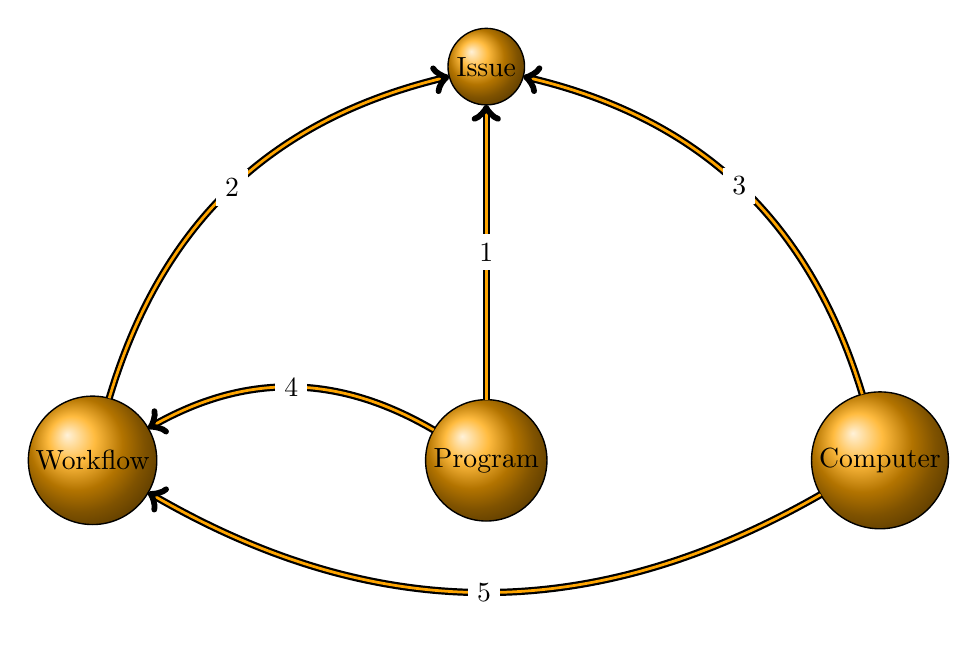
\begin{tikzpicture}
  	   	\GraphInit[vstyle = Shade]
  	   	\SetGraphUnit{5}
  	   	\Vertex{Issue}
  	   	\SOWE(Issue){Workflow}
  	   	\SO(Issue){Program}
  	   	\SOEA(Issue){Computer}
  	   	
  	   	
  	   	\Edge[label = 1, style={<-}](Issue)(Program)
  	   	\Edge[label = 2, style={<-,bend right}](Issue)(Workflow)
  	   	\Edge[label = 3, style={<-,bend left}](Issue)(Computer)
  	   	%\Edge[label = 4](Issue)(Computer)
  	   	%\Loop[dist = 4cm, dir = NO, label = 5](Computer.west)
  	   	%\Loop[dist = 4cm, dir = SO, label = 6](Program.east)
  	   	%\tikzset{EdgeStyle/.append style = {bend left = 50}}
  	   	\Edge[label = 4,style={<-,bend left}](Workflow)(Program)
  	   	\Edge[label = 5,style={->,bend left}](Computer)(Workflow)
  	   	%\Loop[dist = 4cm, dir = SOWE, label = 6](Program.west)
  	   \end{tikzpicture}}
  	\end{column}
  \end{columns}	
\end{frame}

%%%%%%%%%%%%%%%%%%%%%%%%%%%%%%%%%%%%%%%%%%%%%%%%%%%%%%%%%%%%%%%%%%%%%%%%%%%%%%%%
\begin{frame}
  \frametitle{What is the Nature of the Issue?}
  \texttt{Snakemake} helps you to identify the nature of an issue:
  \begin{enumerate}[<+->]
  	\item It will report to you in which \altverb{rule} the error occurred \textbf{and/or}
  	\item a so-called "traceback" to point the issue within its code.
  	\item The workflow will indicate log files on the screen.
  \end{enumerate}
  \pause
  \begin{docs}{Looking into Log Files}
  	Look into the log file. It \textit{should} tell you the error. \pause If not, report it to the workflow developer (next slides). 
  \end{docs}
\end{frame}

%%%%%%%%%%%%%%%%%%%%%%%%%%%%%%%%%%%%%%%%%%%%%%%%%%%%%%%%%%%%%%%%%%%%%%%%%%%%%%%%
\begin{frame}
  \frametitle{Do I need a \texttt{GitHub} account?}
  Today many software projects are either hosted on the global git server, \texttt{GitHub}.
  \begin{docs}
  	If you want to report an issue or even contribute back to the project, you will need an account. \lhref{https://docs.github.com/en/get-started/onboarding/getting-started-with-your-github-account}{This page} describes how. 
  \end{docs}
  
\end{frame}

%%%%%%%%%%%%%%%%%%%%%%%%%%%%%%%%%%%%%%%%%%%%%%%%%%%%%%%%%%%%%%%%%%%%%%%%%%%%%%%%
\begin{frame}
	\frametitle{Reporting Cluster Issues}
	\begin{question}[Where to?]
	  Report them to your cluster admins (\includegraphics[height=\texorpdfstring{\fontcharht\font`\B}]{logos/mattermost.png} chat, \Email{} mail ticket, etc.)
	\end{question}
    \pause
    \begin{question}[What?]
      Inaccessible paths (file system issue), network issues, node failures, etc. 
    \end{question}
    \pause
    \begin{question}[How?]
      Give a meaningful statement. "I can't do \altverb{ls} on \altverb{/some/path}." is more meaningful than "The filesystem stopped working!"\newline
      \bcattention Check your \Email{}! Has some maintenance been scheduled?
    \end{question}	
\end{frame}

%%%%%%%%%%%%%%%%%%%%%%%%%%%%%%%%%%%%%%%%%%%%%%%%%%%%%%%%%%%%%%%%%%%%%%%%%%%%%%%%
\begin{frame}
	\frametitle{Reporting Application Issues}
	\begin{question}[Where to?]
		The issue tracker of your application (if any). 
	\end{question}
	\pause
	\begin{question}[What?]
		Any application specific error. Try running the application with the input and parameters specified in the workflow (get them with \altverb{snakemake -p} to print the shell command or other debug flags). If the application breaks, report the failure. Else, it might be the workflow.
	\end{question}
	\pause
	\begin{question}[How?]
		Indicate the error message and what is leading to it. If you need special input to reproduce the issue, upload the input somewhere or attach minimal input to the issue report.
	\end{question}
\end{frame}

%%%%%%%%%%%%%%%%%%%%%%%%%%%%%%%%%%%%%%%%%%%%%%%%%%%%%%%%%%%%%%%%%%%%%%%%%%%%%%%%
\begin{frame}
	\frametitle{Reporting Workflow Issues}
	\begin{question}[Where to?]
		The issue tracker at your workflow. For \texttt{Snakemake} somewhere in the \lhref{https://snakemake.github.io/snakemake-workflow-catalog/}{catalog}. 
	\end{question}
	\pause
	\begin{question}[What?]
	   Check that it is you causing the error, e.\,g. undefined variables. \texttt{Snakemake} will inform you about the nature of the issue. Read the error output carefully. Report when sure it is not you.
	\end{question}
	\pause
	\begin{question}[How?]
		Indicate the error message and what is leading to it. If you need special input to reproduce the issue, upload the input somewhere or attach minimal input to the issue report.
	\end{question}
\end{frame}

%%%%%%%%%%%%%%%%%%%%%%%%%%%%%%%%%%%%%%%%%%%%%%%%%%%%%%%%%%%%%%%%%%%%%%%%%%%%%%%%
\begin{frame}
  \frametitle{Reporting \texttt{Snakemake} Issues}
  \begin{question}[Where to?]
  	 The \lhref{https://github.com/snakemake/snakemake/issues}{issue tracker of the \texttt{Snakemake} project}.
  \end{question}	
  \pause
  \begin{question}[What?]
  	Clearly unexpected behaviour. Or tracebacks pointing to \texttt{Snakemake} itself. 
  \end{question}
  \pause
  \begin{question}[How?]
  	Indicate the error message and what is leading to it (e.\,g. the command line you used). If you need special input to reproduce the issue, upload the input somewhere or attach minimal input to the issue report.
  \end{question}
\end{frame}


<+++ if course.question is defined +++>%%%%%%%%%%%%%%%%%%%%%%%%%%%%%%%%%%%%%%%%%%%%%%%%%%%%%%%%%%%%%%%%%%%%%%%%%%%%%%%%
\section*{Question Time}
{   
	\usebackgroundtemplate{
		\vbox to \paperheight{\vfil\hbox to \paperwidth{\hfil\includegraphics[height=\paperheight]{humor/DALLE_programming_class_question_time.jpg}\hfil}\vfil}
		% source: https://en.m.wikipedia.org/wiki/File:Text-x-python.svg
	}
	\frame{
		\frametitle{A Chapter ended \ldots}
		\vspace{8.5em}
		\begin{mdframed}[tikzsetting={draw=white,fill=white,fill opacity=0.8,
				line width=0pt},backgroundcolor=none,leftmargin=0,
			rightmargin=50,innertopmargin=4pt,roundcorner=10pt]
			Which questions do you have?
		\end{mdframed}
	}
}<+++endif+++> 

%%%%%%%%%%%%%%%%%%%%%%%%%%%%%%%%%%%%%%%%%%%%%%%%%%%%%%%%%%%%%%%%%%%%%%%%%%%%%%%% 
\begin{frame}<handout:0> 
	\frametitle{The End}
	\begin{center}
		\begin{figure}
			\centering
			
			\includegraphics[width=0.7\textwidth]{logos/the_end.jpg}
		\end{figure}
		Thank you for your attention!
	\end{center}
\end{frame}

\begin{frame}<beamer:0> 
	\frametitle{End of the Talk}

\end{frame}

\end{document}

